\documentclass[12pt,a4paper, twoside,openright]{report}
  \usepackage{fontenc}
  \usepackage{pdfpages} %for titlepage
  \usepackage[utf8]{inputenc}
  \usepackage{float}
  \usepackage{physics}
  \usepackage{amsmath}
  \usepackage{mathtools}
  \usepackage{amsfonts}
  \usepackage{amssymb}
  \usepackage{graphicx}
  \usepackage{csquotes}
  \usepackage{hyperref}
  \usepackage{subfigure}
  \usepackage{rotating} %for rotating images
  %\\usepackage{subcaption}
  \usepackage{fancyhdr}
  \pagestyle{fancy}
  \fancyhead{}
  \fancyhead[RE]{\leftmark}
  \fancyhead[LO]{\rightmark}
  \fancyfoot{}
  \fancyfoot[C]{\thepage}
  \usepackage{gensymb} %degree symbol
  \usepackage[%
  backend=biber,
  style=numeric,
  natbib=true,
  backref=false,
  backrefstyle=all+,
  hyperref=true,
  citestyle=numeric,
  maxcitenames=2,
  sorting=none,
  ]{biblatex}
  %\renewcommand\nametitledelim{\ifin{textcite}{\addspace}{\addspace\addcomma}}
  \renewcommand*{\nameyeardelim}{\addspace}
  \renewcommand{\floatpagefraction}{.8}%less floaty images
  
  \addbibresource{bibliography.bib}
  \linespread{1.2}
 
  \binoppenalty=\maxdimen
  \relpenalty=\maxdimen %don't break equations
 \begin{document}
 	\includepdf{titlepage}
 	\chapter*{Abstract}

The MariX project consists in the development of two new X-ray sources: a high-repetition rate Free Electron Laser (whom applications are in ultra-fast linear spectroscopy, cristallography, pump-probe experiments and spectroscopy) and an Inverse Compton Scattering source (with applications in medical research and radiotherapy, cultural heritage and material science). In particular the ICS source, called BriXS, will also be used for K-edge subtraction (KES) contrast imaging, a diagnostic method exploiting the sharp change in a intravenous contrast agent used for example in cancer detection.

The ICS process requires high-photon flux to produce high energy (up to 180\,keV) X-ray photons, this can be achieved using a Fabry-Perot cavity, an enchantment resonator. KES imaging requires two different X-ray energies to be produced in temporal proximity and the Compton process presents a dependence on the interaction angle that can be exploited for this dual-color X-ray production. The solution that we propose consists in using two crossed Fabry-Perot optical cavities, switching between the two by the means of moving mirrors, in order to generate photons at both 32\,keV and 34\,keV, the energies needed for iodine KES.

In this thesis work, we built two crossed 4-mirrors bow-tie Fabry-Perot resonators and stabilized them against a mode-locked laser source using the Pound-Drever-Hall (PDH) technique. The cavities have then been characterized, measuring important parameters such as the cavity Finesse, the power spectral density noise, the mirror reflectivities and the spatial and spectral coupling with the laser beam. The latest cavity model reaches a Finesse of about 3000 and an integrated frequency noise of 3500\,Hz, giving a relative frequency fluctuation between cavity and laser of the order of $10^{-11}$. The method to switch the cavity interacting with the electron beam has been studied and experimentally tested, it consists in moving the cavities foci in and out of the interaction point using piezo driven mirrors while the cavity remains stabilized with the source. We obtained a movement of 80\,$\mu$m in under 100\,ms, indicating the feasibility of the method. Also a technique for dealing with high power effects such as thermal deformation of the mirrors and degenerate mode coupling losses has been developed and tested, again with positive results.

In the first chapter an overview of the MariX project is given, with attention on the laser system that drives both the FEL and ICS sources. In the second chapter I explain the theoretical concepts necessary to understand the experimental results, they concern mainly the inverse Compton scattering process and the physics of optical resonators and laser beams. Theoretical predictions are also given, regarding the expected results and possible obstacles in future developments. The third chapter is a brief study on the cavities stabilization systems and the PDH technique, given its importance in the experimental apparatus. In the fourth chapter, I present the experimental setup and results obtained during the thesis work. Finally, in the conclusions I highlight the next steps to be taken in the R\&D program.


 	\chapter*{}
 	\begin{flushright}
 		Ai miei genitori, Franca e Andrea
 	\end{flushright}
 	\tableofcontents
	\chapter{Introduction}
To establish the framework in which this thesis has been developed, a general overview of the MariX project\footnote{For an extended overview of the project the Conceptual Design Report \parencite{CDR} is available at \url{https://marix.mi.infn.it}} (Multi-disciplinary Advanced Research Infrastructure for the generation and application of X-rays) is given, with a focus on the Laser system.
\section{The MariX project}
X-rays has been used for decades to study the structure of matter, enabling for example spectroscopy and nanometric imaging. Typical modern X-ray production utilizes accelerated electrons either in 3rd generation storage ring light sources, based on synchrotron acceleration, or in 4th generation Free Electron Laser (FEL) sources, based on linear accelerators (linac) and self-amplification of spontaneous emission (SASE).

The MariX project aims to provide a new generation of X-ray source capable of producing coherent, ultra-high flux, femtosecond-class radiation, with photon energies spanning from 300\,eV (soft X-rays) to 180\,keV (hard X-rays). Such characteristics will be achieved by combining two different radiation production mechanism:
\begin{itemize}
	\item a FEL source will produce coherent ultra-short ($<10^{-14}$\,s) pulses in the 200\,eV - 8\,keV region, with a repetition rate of up to 1\,MHz and a flux of up to $10^{18}$ photons/s;
	\item an Inverse Compton Scattering (ICS) source will produce picosecond pulses in the 20\,keV - 180\,keV region, with a repetition rate of 100\,MHz and a flux of up to $10^{13}$ photons/s.
\end{itemize}
\begin{figure}
	\centering
	\includegraphics[width=0.9\linewidth]{images/fel.png}
	\caption{Layout of the MariX-FEL source: the bubble-arc compressor sends the electrons back into the linac to be accelerated a second time, reaching energies of up to 3.2-3.8\,GeV. Picture from \parencite{CDR}}
	\label{fig:fel}
\end{figure}

As the name suggests, the project is multi-disciplinary in nature and will advance research in a variety of fields, such as: femto-second time resolved linear spectroscopy, protein and nano-object imaging at nano-scale resolution, advanced radiological imaging with multi-color X-rays, new radio-therapy techniques with tunable mono-chromatic hard X-rays.
In particular the characteristics of the FEL source make it ideal for ultra-fast linear spectroscopy, which requires time resolution of 10-100\,fs to study the behavior of excited matter during various transients, but also demands the number of photons per pulse to remain within the limits of linear response. Currently available FEL sources have pulses that exceeds this limits by 2-4 orders of magnitude, and so significant power is wasted as they need to be attenuated, while synchrotron radiation sources don't have the required temporal resolution (current pulses are in the few tens of ps range). MariX-FEL will fill this gaps in time resolution and average photon flux, delivering radiation in continuous wave (CW) mode at 1\,MHz, a high repetition rate that will be useful for collecting adequate statistics in short times.

The applications for the ICS source come from its ability to deliver high-brilliance monochromatic tunable X-rays, which production is usually left to expensive and large synchrotron facilities. In particular, this kind of radiation has been proven to be of great interest for medical research in radiology and radiotherapy, but also for biology, cultural heritage and material science. This source will provide radiation with synchrotron-like features while being both much smaller (about 100\,m$^2$) and cheaper (tens of millions of euros) to construct and operate (current synchrotron facilities occupy 100 times this area and cost about 10 times more).
Another challenge for the MariX project is the space available: the dimensions of the whole facility are limited to about 500\,m in length. Existing linacs typically have a length of a few kilometers to achieve an electron beam energy of 10-20 GeV; to address this problem a new scheme of folded linac enabled by a bubble-arc compressor  has been developed (as represented in Fig \ref{fig:fel}), this will reduce the length required to less than 500\,m for a maximum electron energy of 3.8\,GeV.

\section{BriXS (Bright compact X-rays Source)}
\begin{figure}
	\centering
	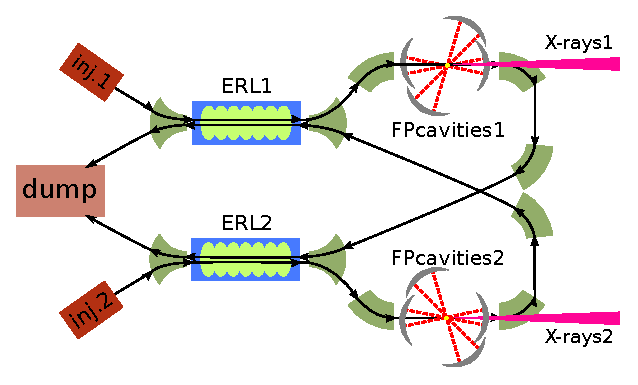
\includegraphics[width=0.9\linewidth]{images/BriXS.eps}
	\caption{Layout of BriXS, the MariX-ICS source: the energy recovery linacs accelerate the electrons to up to 300\,MeV, magnetic quadrupoles then guide the bunches to the Fabry-Perot cavities where X-Rays are produced. In each branch there are two crossed cavities in order to operate in dual-color mode.}
	\label{fig:brixs}
\end{figure}
BriXS is the name of the MariX inverse Compton scattering X-ray source, it is being developed with the aim of providing a synchrotron-like light source with limited footprint (laboratory-sized) and costs. His compactness and affordability will greatly benefit small research institutions and clinics, enabling innovative research and medical diagnosis and therapy.

BriXS radiation will be tunable in energy (20\,keV - 180\,keV), with a relative bandwidth of $\Delta E/E = 1-10\%$ and intensities  of $10^{11}-10^{13}$ photons/s. The beam will have a higher divergence than typical synchrotron light (10x10\,cm$^{2}$ at less than 100\,m from the interaction point), this is useful in medical application where uniformity and broadness of the light is required to allow single-shot imaging.
One of the key features of BriXS, and the main one addressed in this thesis, will be the production of X-rays with two different energies (``colors'') with a fast switch time between the two. Dual color X-rays can be used to probe matter in pump-probe experiments, but also to provide better biomedical imaging such as in K-edge color subtraction and microtomography \parencite{Jacobson1953}.
In pump and probe experiments one pulse (pump) is used to excite atoms in the sample to a higher energy state, while a different second pulse (probe) is used to study the atomic, electronic and magnetic structure of the sample.
K-edge subtraction (KES) imaging exploits the sudden change in the absorption coefficient of a contrast agent at a precise energy. An image is taken with X-rays just below the K-edge energy and then another with X-rays just above. The attenuation coefficient of the tissue doesn't vary much with energy, while that of the contrast agent changes sharply. By combining these two by logarithmic subtraction it is possible to produce hybrid images that highlight the contrast agent, while unwanted structures have their contrast reduced \parencite{Lehmann1981}. Both acquisition are made after the injection of the contrast agent and in temporal proximity to avoid patient/sample movement. The main clinical application of KES is today coronary angiography where iodine is used as the contrast agent thanks to its absorption edge at 33.17\,keV (see Fig \ref{fig:iodine}). Coronary angiography is extremely useful in cancer detection, in particular for breast cancer: in fact in some cases screening mammography proves ineffective in finding the tumor, while KES can easily identify the extra blood vessels formed around it \parencite{Lewin2003}. Having explained the importance of KES, the aim of this thesis is to develop the system that will enable BriXS to easily and swiftly shift between the two radiation energies. Since iodine contrast imaging is our objective, the radiation will be tailored to its K-edge energy, at 32 and 34\,keV.
\begin{figure}
	\centering
	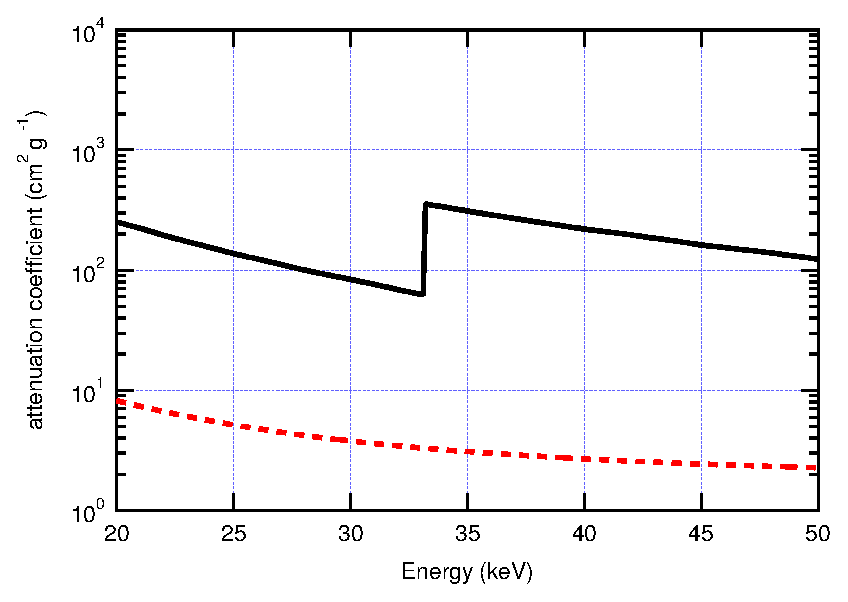
\includegraphics[width=0.9\linewidth]{images/iodine.eps}
	\caption{Linear attenuation coefficient as a function of photon energy. For iodine (solid black) a sharp absorption edge is present at 33.17\,keV, while it is absent for soft tissue (dashed red). Image is taken from \parencite{CDR}}
	\label{fig:iodine}
\end{figure}

Other applications of BriXS include Phase Contrast imaging, in which the sample internal structure is probed by measuring the phase shift it introduces on the radiation, radiotherapy, in particular breast cancer rotational radiotherapy which is now available only in a few centers in the world, X-ray fluorescence and diffraction experiments.

The structure of the BriXS facility is represented in Fig \ref{fig:brixs}, it has two symmetric beam lines in which electron bunches are produced in two injectors with repetition rate of 100\,MHz resulting in an average current of 20\,mA. The beams are then accelerated through two Energy Recovery Linacs (ERL) towards the interaction point (IP). Here the electrons interact with the photons inside two Fabry-Perot cavities (for a total of four cavities) and generate X-rays through inverse Compton scattering. The beams are then reinserted in the opposite ERL where they are decelerated and their energy recuperated. This coupled scheme permits to drive two independent Compton sources while simultaneously being more stable than a single ERL scheme.
The injectors for BriXS and the FEL and the Fabry-Perot cavities use the radiation produced by the Laser system, which includes Laser oscillators and cavities.

\section{The Laser system}
\begin{figure}
	\centering
	\includegraphics[width=1\linewidth]{images/pm.pdf}
	\caption{The MariX Laser system}
	\label{fig:photonic}
\end{figure}
Both MariX sources are driven by the Laser system, which uses a single laser oscillator as seed. The oscillator is mounted on an optical table, while the Fabry-Perot cavities are placed at the Interaction Points. The scheme also includes the fiber amplifiers, the temporal and spatial shaping system for the RF-guns, a Mach-Zender amplitude modulator, and two stabilization feedback systems.

The purpose of this optical system is to provide adequate radiation pulses in order to generate the electron bunches needed for both the FEL and the ICS source, but also to pump the optical cavities to the power necessary for the scattering process. Using a single laser source yields the advantage of having intrinsic synchronization between the laser pulses and the electron bunches. The light coming from the mode-locked pulsed laser is divided into three lines: one dedicated to the resonant cavities, one to the two RF-guns for the Compton source, and one to the RF-gun for the FEL. Each line will have a power of about 100\,mW before being amplified through multiple fiber amplifier stages. The repetition rate of the oscillator is 100\,MHz, in the FEL line it is reduced to 1\,MHz by the means of the Mach-Zender amplitude modulator.
Before entering the Fabry-Perot cavities the power is brought to about 200\,W, once inside the cavity the light pulses are superimposed with each other and the power reaches a value determined by the cavity Finesse, from 1000 to 10000 times the input power. In MariX we aim to obtain an enhancement factor of at least 2500, that is an average power of 500\,kW inside the cavity, and to possibly get to even higher figures.
The Compton RF-guns line is also amplified to 200\,W before being upshifted to the $4^{th}$ armonic by the means of two non-linear crystals. The pulse is then temporally and spatially shaped to achieve maximum efficiency in the photoelectric process. The FEL line is similar but the power is lower: about 1\,W at 1\,MHz, the pulse is also upshifted and shaped.

The cavities are stabilized against the laser using the Pound-Drever-Hall (PDH) technique \parencite{Black2001}, this is needed as the cavity electromagnetic modes needs to exactly match the oscillator modes. Another feedback system is used to synchronize the laser oscillator with an external reference.

\subsection{Laser oscillator}
A pulsed laser (as opposed to a continuous wave laser) is used in order to reach the high photon flux for the Compton process and the electronic bunches production. The oscillator of choice is a Yb-fiber mode-locked laser, delivering 100-200\,fs pulses\footnote{The oscillator in our laboratory has an in-built compressor to regulate the pulse length. Using an autocorrelator we measured a minimum pulse length of 130\,fs.} at 100\,MHz on a carrier wavelength of 1030\,nm. To reach maximum coupling with the Fabry-Perot cavities the laser beam must be single mode and have a spatial profile as similar to that of the cavity fundamental mode\footnote{Cavity modes theory will be dealt with in the next chapter.} (TEM$_{00}$) as possible, that is with a beam quality factor $M^2$ close to 1, where $M^2=1$ represents a perfectly gaussian intensity profile. Any mode non resonant in the cavity will not be coupled, that is reflected by the input mirror and its power wasted. Since we want the ICS source to be controllable in polarization we need it to have a high degree of polarization (close to  100\%), the source must also have good pointing stability and pulse to pulse stability. An Yitterbium-fiber laser meets this requirements: the fiber (which is also the gain medium) guides the beam propagation making it reach excellent spatial quality and simultaneously maintaining the beam polarization. The fiber can be pumped with laser diodes at 975\,nm with great quantum efficiency, reducing the power wasted into heat. This means that the system doesn't need extreme cooling and is compact.

To explain why the stabilization systems are needed we need to describe the mode-locked laser pulses in the temporal and spectral domain. In the time domain the pulses can be described by the oscillation at the carrier frequency $f_c$ and the periodic intensity envelope with period $T$. The phase shift between the two $\Delta\Phi_{CEO}$ is called carrier-envelope offset. In the frequency domain the pulses can be described by the repetition rate $f_{rep}=1/T$ and the $f_{CEO}=\Delta\Phi_{CEO} f_{rep}/2\pi$. The frequency comb is then:
\begin{align}
f_m = m f_{rep} + f_{CEO} = \left(m  + \frac{\Delta\Phi_{CEO}}{2\pi}\right) f_{rep}
\end{align}
To control the frequency comb a fine tuning of both $f_{rep}$ and $\Delta\Phi_{CEO}$ is necessary, the former to synchronize the laser with a reference and the latter to match the laser modes with the cavity modes.
The comb experiences fluctuations caused by pump and quantum noise, mechanical vibrations and nonlinear effects of the gain medium; the purpose of the two feedback stabilization systems is to compensate this fluctuations.

Oscillators with the requested characteristics are available on the market: both the Orange Menlo and the Origami One Five are candidates for the role. In our laboratory we currently use the Orange laser for R\&D purposes.

\begin{figure}
	\centering
	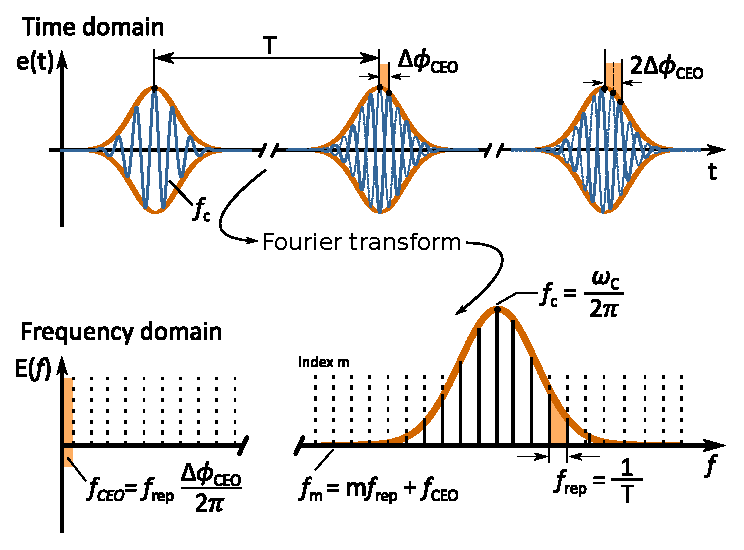
\includegraphics[width=0.9\linewidth]{images/comb.eps}
	\caption{Representation of a mode-locked laser pulse in the time domain and its frequency comb in the Fourier domain.}
	\label{fig:comb}
\end{figure}

\subsection{Fiber amplifiers}
To amplify the pulses to the requested power the Chirped-Pulse-Amplification (CPA) technique \parencite{Strickland1985} will be used\footnote{For developing the CPA technique, Donna Strickland and Gérard Mourou have been awarded the 2018 Nobel Prize in physics “for their method of generating high-intensity, ultra-short optical pulses”.}.
In this scheme the pulses are stretched temporally by introducing a linear chirp, delaying each frequency by a different amount. This reduces the maximum power of the pulse in order to avoid fiber damage and non-linear effects such as self-phase modulation (SPM) that can spoil the spatial quality of the beam.
\iffalse We can describe the electric field of a simple gaussian pulse as superposition of monochromatic waves. Since the Fourier transform of a gaussian curve is also gaussian we have:
\begin{align}
E(t) = \mathrm{e}^{-\frac{\omega^2}{\sigma^2}} \mathrm{e}^{i\omega t}
\end{align}
To introduce a linear chirp we make the substitution $t\rightarrow t-\alpha\omega$:
\begin{align}
E(t) = \mathrm{e}^{-\frac{\omega^2}{\sigma^2}} \mathrm{e}^{i\omega (t-\alpha\omega)} = \mathrm{e}^{-\frac{\omega^2}{\sigma^2}} \mathrm{e}^{-i\alpha\omega^2} \mathrm{e}^{i\omega t}
\end{align}
\fi
The stretching of the pulse can be achieved with chirped volume Bragg gratings (CVBG), which are diffraction gratings engraved into a monolithic crystal that reflect different wavelengths at different positions, as represented in Fig \ref{fig:CVBG}.
\begin{figure}
	\centering
	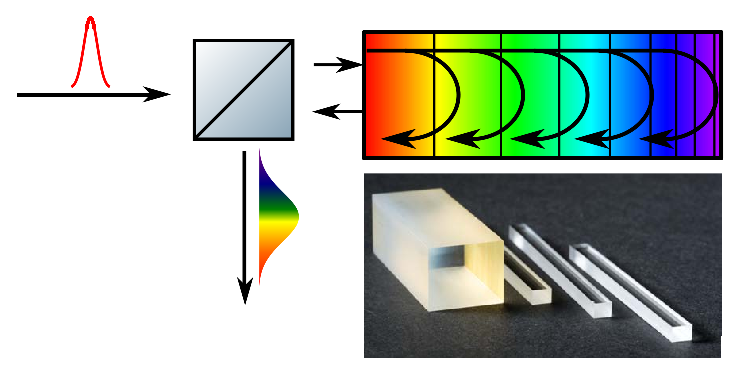
\includegraphics[width=0.9\linewidth]{images/CVBG.eps}
	\caption{Chirped Volume Bragg Grating: a short laser pulse that enters a CVBG is stretched as its spectral components are delayed differently depending on the frequency. Another CVBG can be used to compress the pulse to its original length after amplification. CVBG are engraved into monolithic crystals as displayed in the lower picture.}
	\label{fig:CVBG}
\end{figure}
The chirped pulse is then coupled in a large mode area (LMA) polarization maintaining double clad fiber. The fiber is composed by a single mode Yb-doped inner core (the gain medium) in which the pulse to be amplified is coupled, and a larger multi-mode cladding in which the laser pump is launched. By coupling the pump in a larger area than the seed nonlinear effects and fiber damage are avoided, in addition the pump source doesn't need to be single mode and can be launched efficiently thanks to a big numerical aperture \parencite{Paschotta1997}. The Yb-doped fiber allows up to 7\,dB/m amplification at a pump wavelenght of 975\,nm, with a typical conversion efficiency of 60\%.
The amplified pulses are then compressed with another CVBG, reducing the chirp to reach the desired pulse length; in our Compton source we need a pulse length of a few ps (to match that of the electron bunch) while for the RF-Guns tens of ps are required.
\begin{figure}
	\centering
	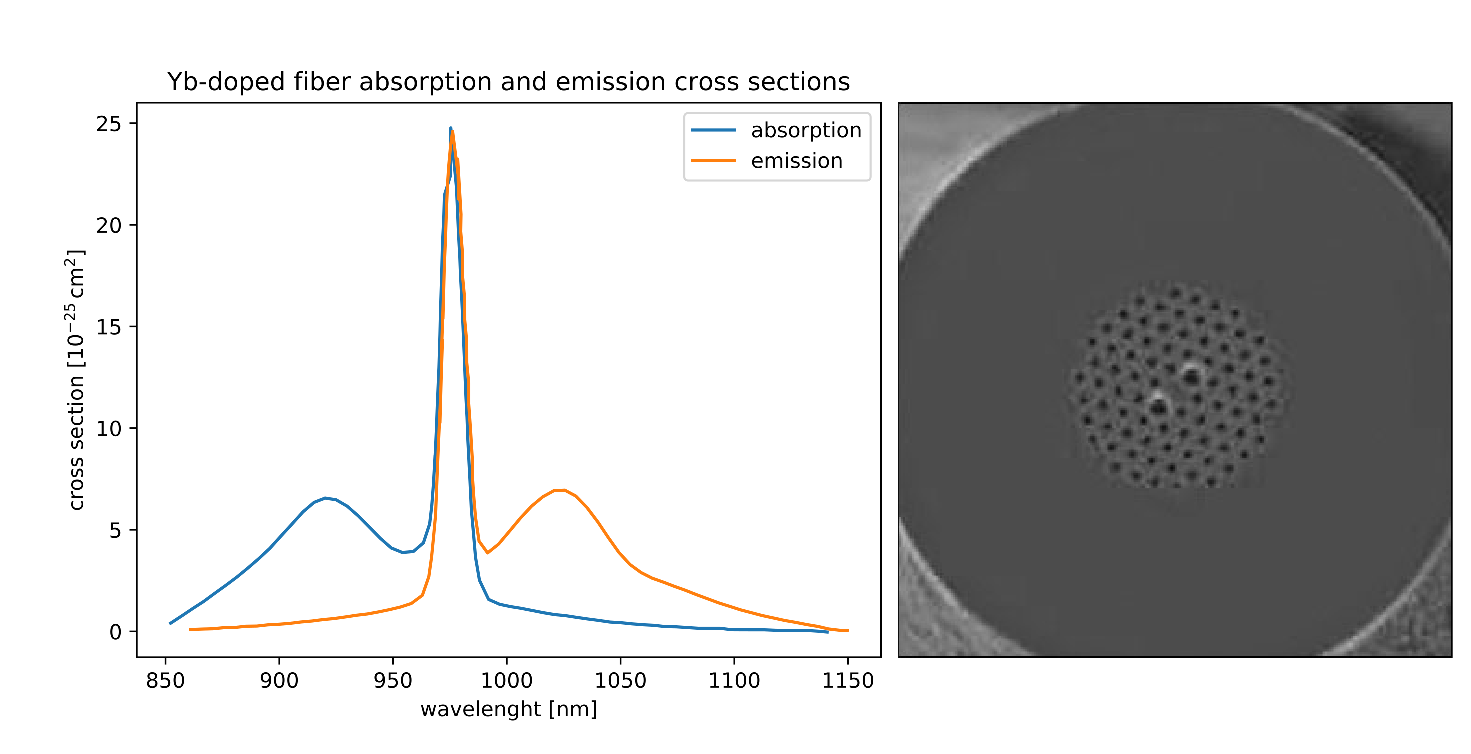
\includegraphics[width=0.9\linewidth]{images/ybfiber.eps}
	\caption{On the left: typical absorption and emission cross sections for a Yb-doped fiber. The large emission spectrum makes it ideal for ultra-short pulse amplification, maximum pump efficiency is reached at 975\,nm. On the right: a Photonic Crystal Fiber (PCF), in these fibers the index of refraction in the cladding is modified by small air cavities, confining the seed beam in the small core. The PANDA stress rods (the two dots at the center) make the fiber Polarization Maintaining. Picture and data from Thorlabs, Inc.}
	\label{fig:ybfiber}
\end{figure}

The amplifier scheme will be composed of three stages, as different powers need different fiber dimensions and cooling systems. Multiple stages are also needed to reduce noise sources such as SPM and amplified spontaneous emission (ASE). Self-phase modulation arise in fibers when the intensity of the pulse is high because of the Kerr effect, that is the dependence of the refractive index of the medium from the square of the electric field. It can lead to frequency broadening and pulse spreading \parencite{Stolen1978}, but also to bad coupling with the Fabry-Perot cavities modes. Amplified spontaneous emission occurs when the power is low but the gain is high (30-40\,dB according to \parencite{Paschotta1997}) and reduces the total gain while introducing unwanted noise. 
In the cavities and Compton lines, the first stage will bring the 100\,mW seed to about 2\,W, the second will reach 60\,W and the last one will get to 200\,W. Since the first stage has high gain a forward pumping scheme will be used to reduce the effect of ASE \parencite{Paschotta1997}, with the seed and pump beam entering the fiber from the same side. The other stages will instead use a backward pumping scheme to reduce the nonlinear effects in the fiber due to the high power. The two schemes yield the same output power, but in the backward case the average power inside the fiber is lower. While a commercial solution for the first stage is available, the other two stages will be developed in the R\&D phase.

\subsection{Fabry-Perot cavities}
\begin{figure}
	\centering
	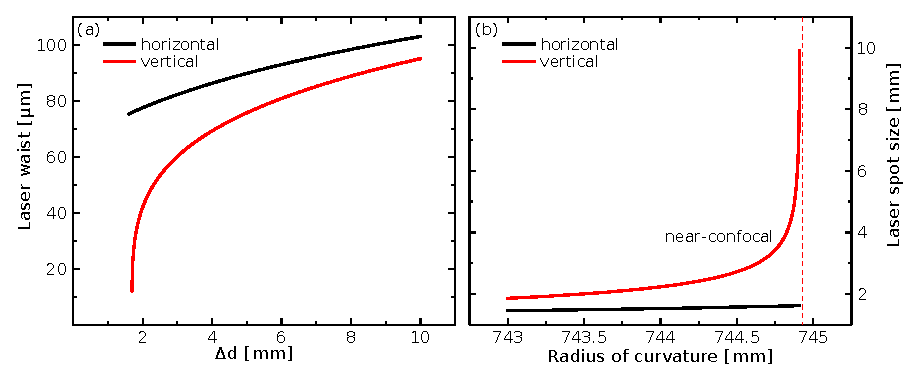
\includegraphics[width=0.9\linewidth]{images/waistspot.eps}
	\caption{(a) The laser beam spot size at the waist as a function of the distance between the curved mirrors. (b) The spot size at the mirror surface as a function of the mirrors radius of curvature.}
	\label{fig:waistspot}
\end{figure}
To reach the high photon flux needed for the Compton process a Fabry-Perot optical cavity can be used.
In an optical cavity the electromagnetic field can exist in stationary states called modes. Modes have well-defined wavelength and spatial profiles that must be matched to couple an external laser beam to a cavity. In the case of a pulsed laser the temporal matching condition must also be met, that is an incoming pulse must exactly overlap with the pulse resonating in the cavity. In the frequency domain this condition means that the pulse spectral comb must match the cavity spectral comb. After each round trip the intensity of the pulse inside the cavity increases until equilibrium is reached between gain and losses. The temporal condition fixes the cavity length to the inverse of the repetition rate of the laser multiplied by the speed of light (or a multiple of this quantity):
\begin{align}
L = m \frac{c}{f_{rep}}
\end{align}
In our case we want a single pulse inside the cavity to achieve maximum peak power ($m=1$):
\begin{align}
L = \frac{c}{f_{rep}} \approx \frac{3*10^8\,\mathrm{m/s}}{100\,\mathrm{MHz}} = 3\,\mathrm{m}
\end{align}
\begin{figure}
	\centering
	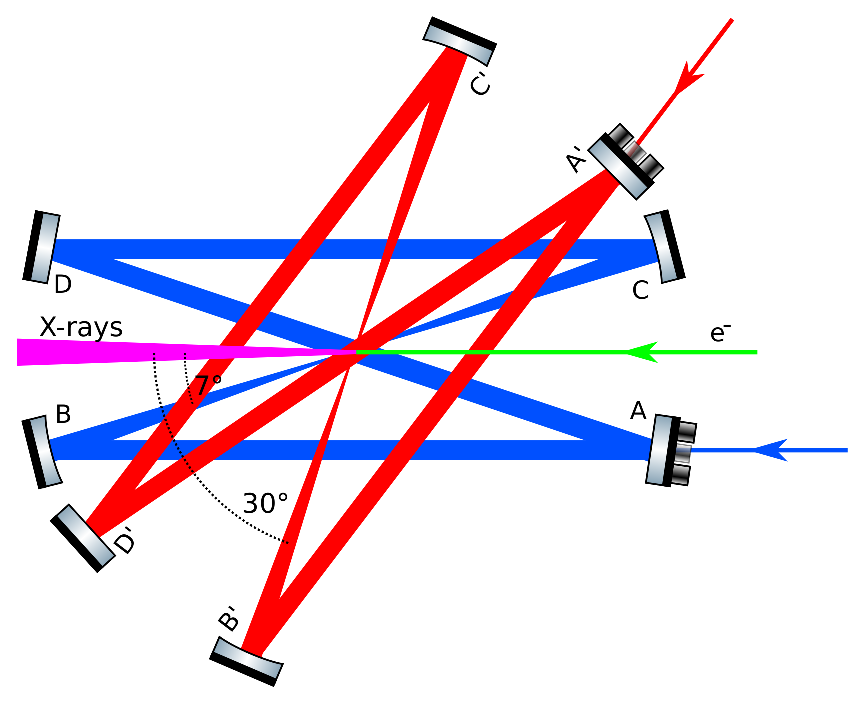
\includegraphics[width=0.9\linewidth]{images/doublecavity.eps}
	\caption{Scheme of the two 4-mirrors bow-tie confocal optical resonators. A and A' are the input couplers; B, B', C, C' are the curved mirrors and the distance between them regulates the spot size at the beam waist; D and D' are flat mirrors and are used to restore the cavities length when changing the distance between the curved mirrors.}
	\label{fig:bowtie}
\end{figure}
The cavity design of choice is a 4-mirrors (2 flat and 2 curved) bow-tie near-confocal cavity. This geometry has the advantage of being stable while also allowing adjustments of the beam waist without changing the length (which influences the resonant frequency) and vice-versa. In a Compton source fine tuning of the beam waist is necessary to better match the electron beam profile at the interaction point, which corresponds to the focus of the cavity. Changing the curved mirrors distance and restoring the length with the flat mirrors also allows to change the laser spot size on the mirrors: a big spot size is desired to avoid thermal deformation of the reflecting surface.

As it will be explained in the next chapter, the frequency of the X-rays produced through inverse Compton scattering presents a strong dependence from the angle between the interacting photons and electrons. We then propose to use two identical crossed Fabry-Perot cavities at two different angles in order to implement the ``dual color mode'', a key feature of BriXS. As represented in Fig \ref{fig:bowtie}, the electrons will pass between two of the first cavity mirrors, interacting with the pulse coming from mirror B at an angle of about 7\degree. To switch from one cavity to the other, we propose to use piezo-electric driven moving mirrors that can move the laser beam in and out of the interaction point. During the switch, the moving mirrors will translate the focus of the first cavity away from the electron beam while simultaneously placing the focus of the second cavity in the interaction zone. The angle of incidence with the second cavity will be about 30\degree, the two angles are chosen in order to bracket the iodine K-edge energy at 32 and 34\,keV. A key point is the fact that the two cavities must remains stabilized (in resonance with the oscillator) during the movement, in the third chapter I will present the experimental results we obtained which indicate that it is possible to switch between the two cavities without losing the matching and coupling with the external laser mode.

\subsection{4th armonic generation}
\begin{figure}
	\centering
	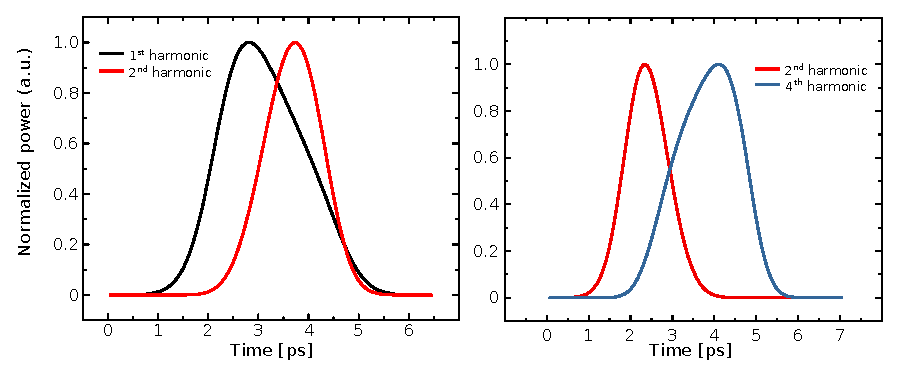
\includegraphics[width=0.9\linewidth]{images/harmonic.eps}
	\caption{Simulation of second and fourth harmonic generation in nonlinear birefringent crystals (LBO and CLBO). The resulting pulse length depend on the length of the crystal.}
	\label{fig:harmonic}
\end{figure}
High electron beam current and brightness require photocathodes with high Quantum Efficiency (QE). The natural choice is then to use semiconductor cathodes that have good QE in the UHV region. To get UHV light from the 1030\,nm pulses 4th harmonic generation through two nonlinear birefringent crystals will be employed, each doubling the frequency of the beam. The 2nd harmonic (515\,nm) will be produced inside a Lithium triborate (LBO, LiB$_3$O$_5$) crystal while the 4th harmonic (257.5\,nm) generation will take place in a Cesium Lithium Borate (CLBO, CsLiB$_6$O$_10$) crystal. Second harmonic generation (SHG) can be achieved when the so-called phase-matching condition is met: since the crystals are nonlinear an incoming field oscillating at $\omega$ will make the polarization oscillate at $2\omega$, if the two waves propagate at the same phase velocity oscillations generated at different places will interfere constructively and result in a $2\omega$ radiation field exiting the other end of the crystal. The phase-matching condition is then:
\begin{align}
n(\omega) = n(2\omega)
\end{align}
This condition is achievable in birefringent materials, that have different indexes of refraction for different field polarization. LBO and CLBO are uniaxial crystals, meaning they have index $n_o$ along two axes and an index $n_e$ along the third. In LBO the noncritical phase-matching can be used since $n_e$ presents a strong dependence on the temperature $T$, if the crystal is kept at a temperature such that $n_o(\omega) = n_e(2\omega,T)$ SHG will take place. In CLBO critical phase-matching can be used instead. If the second harmonic travels at an angle $\theta$ with respect to the crystal axis, it will travel with an index of refraction given by:
\begin{align}
\frac{1}{n^2(2\omega,\theta)} = \frac{\sin^2\theta}{n^2_o(2\omega,\theta)} + \frac{\cos^2\theta}{n^2_e(2\omega,\theta)}
\end{align}
Then for a particular angle the phase-matching condition $n_o(\omega)=n(2\omega,\theta)$ can be satisfied. In this case the extraordinary beam experience walk-off, this effect can be mitigated using two CLBO crystal glued together with opposing orientation. Simulation on the crystals effect on the pulse length are shown in Fig \ref{fig:harmonic}.

\subsection{Temporal shaping}
\begin{figure}
	\centering
	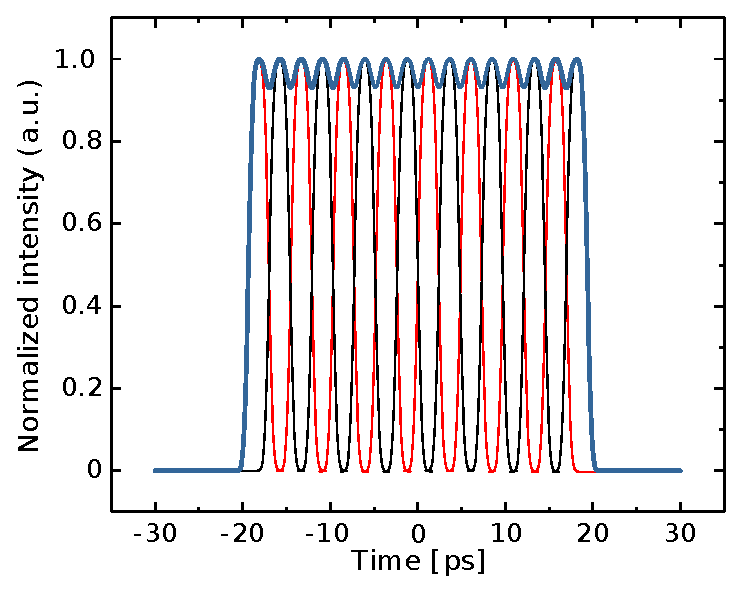
\includegraphics[width=0.9\linewidth]{images/temporal.eps}
	\caption{In this simulation a $\sim$2\,ps pulse is shaped by four $\alpha$-BBO crystals of lengths 22, 11, 5.5, 2.75 nm to get to the 40\,ps figure necessary for the FEL line. Red and black indicate orthogonal polarizations while blue is the sum of the two.}
	\label{fig:temporal}
\end{figure}
To optimize the temporal profile of the pulse for the photoemission process the passive pulse stacking technique can be used. This consists in overlapping replicas of the original pulse to obtain a rectangular-shape pulse and it can be done either with delay lines or with a set of birefringent crystals such as Barium beta borate ($\alpha$-BBO). Since in such a crystal we have two different group velocities for horizontal and vertical polarization, a pulse linearly polarized at 45 degrees will divide in two equal intensity replicas having opposite polarization, with a time separation between the two
\begin{align}
t_d = \frac{1}{c} \left|n_{g,o}L-n_{g,e}L\right|
\end{align}
With $n_g=c\,\partial k/\partial \omega$ being the group refractive index for the two polarizations and $L$ the crystal length.
Further replicas can be obtained adding a second crystal of length $L/2$ and so on until the pulse has the desired length and shape. For the Compton line a pulse of $\sim$20\,ps is desired while for the FEL line $\sim$40\,ps. Since the pulse length is estimated to be 1.6\,ps after the amplification and 4th harmonic generation system a set of three crystals can be used for the Compton line and four for the FEL.

\subsection{Spatial shaping}
\begin{figure}
	\centering
	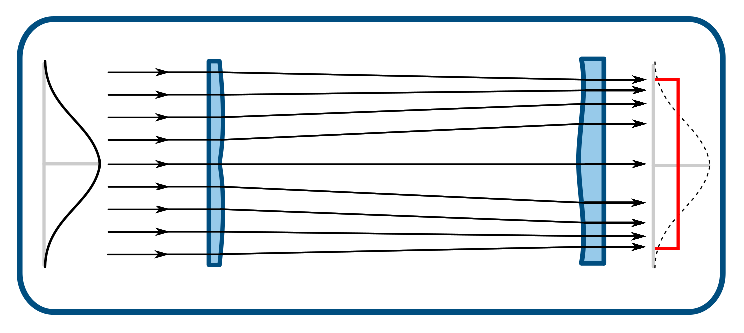
\includegraphics[width=0.9\linewidth]{images/pishaper.eps}
	\caption{$\pi$-shaper: two aspherical lenses can transform a gaussian spatial profile into a flat-top profile.}
	\label{fig:pishaper}
\end{figure}
The intensity profile of the beam can be modified with a set of two aspherical lenses, in particular a commercially available $\pi$-shaper can modify a gaussian beam into a flat-top beam.
Since such a beam is not a free-space mode, i.e. its profile is not maintained in free-space propagation, a telescopic system must be used to reproduce its rectangular profile on the photocathode.
\begin{figure}
	\centering
	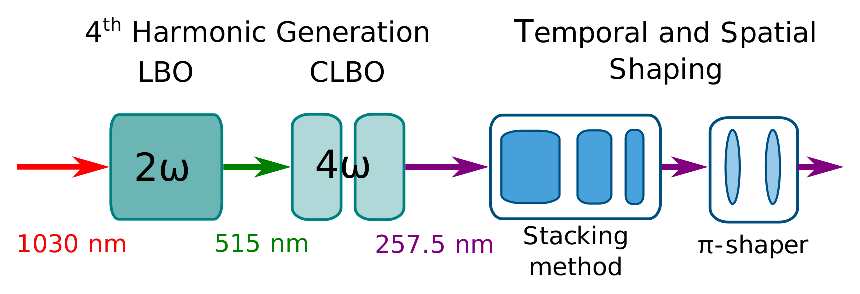
\includegraphics[width=0.9\linewidth]{images/rfgun.eps}
	\caption{Transformation of the pulse for the RF-guns line: firstly two second harmonic generation stages bring the wavelength to 257.5\,nm, then temporal and spatial shaping modify the pulse longitudinal and transverse profile to optimize the photoemission process.}
	\label{fig:rfgun}
\end{figure}

\subsection{Mach-Zender amplitude modulator}
\begin{figure}
	\centering
	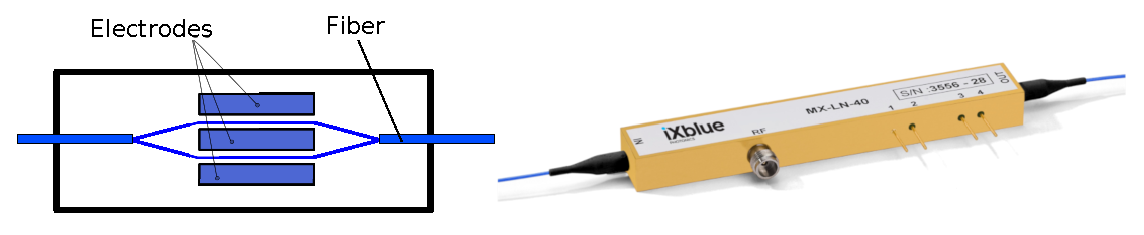
\includegraphics[width=0.9\linewidth]{images/mach.eps}
	\caption{Example of a Mach-Zender amplitude modulator.}
	\label{fig:mach}
\end{figure}
The FEL RF-guns line requires the electron bunches to have a repetition rate of 1\,MHz. Since we want to use the 100\,MHz laser oscillator to drive the entirety of the Laser system, a Mach-Zender amplitude modulator con be used to reduce the repetition rate to the desired level. Such a modulator is in fact an interferometer that can introduce a phase difference between the two paths, leading to constructive of destructive interference. To change the relative phase materials like Lithium niobate (LiNbO$_3$), which has a refractive index strongly dependent on the applied electric field, can be used. By applying an electric field with the right intensity and timing only 1 every 100 pulses exits the interferometer.

\subsection{Stabilization systems}
In order for the laser oscillator to have a stable repetition rate $f_{rep}$ it needs to be synchronized with an external radio-frequency source or with an optical source. The time jitter is about 150\,fs for the former solution and a few fs for the latter. Such solutions are commercially available and an example is shown in Fig \ref{fig:synchro}.
\begin{figure}
	\centering
	\includegraphics[width=0.9\linewidth]{images/synchro.eps}
	\caption{Scheme and picture of the synchronization module for the Orange Menlo laser by Menlo Company. It generates an error signal comparing the phase difference with the laser and acts on the oscillator with two actuators: a piezo and a mechanical stage.}
	\label{fig:synchro}
\end{figure}

The other stabilization system deals with the mode matching between the cavity and the laser source. Thermal effects and mechanical noise modify the length of the cavity that needs real-time correction, but also source noise must be corrected.
We recall that the frequency comb of the oscillator is:
\begin{align*}
f_m = m f_{rep} + f_{CEO}
\end{align*}
while that of the cavity is:
\begin{align}
f_{cm} = m f_{FSR}
\end{align}
where $f_{FSR} = c/L$ is the Free Spectral Range of the cavity, that is the distance in frequency between two TEM$_{00}$ modes of the cavity and depends only on the cavity length.
The matching condition for a mode identified by the index $m_0$ is then:
\begin{align}
m_0 f_{rep} + f_{CEO} = m_0 f_{FSR}
\end{align}
From which is clear that fine stabilization of the cavity length is needed to maintain $f_{FSR} = f_{rep} + f_{CEO}/m_0$. A typical value for $m_0$ would be $L/\lambda = 3\times10^6$.
For a mode-locked laser, the pulse is composed of several modes separated by $f_{rep}$, let's calculate the frequency difference between $f_m$ and $f_{cm}$ when $m=m_0+\delta m$:
\begin{align}
\delta f &= (m_0+\delta m)(f_{rep} + f_{CEO}/m_0) - ((m_0+\delta m) f_{rep} + f_{CEO})\\
\delta f &= f_{CEO}\frac{\delta m}{m_0}
\end{align}
Since all the modes in the pulse should match a cavity mode $f_{CEO}$ should be kept as low as possible, ideally at 0. To control both $f_{FSR}$ and $f_{CEO}$ a double PDH \parencite{Black2001} system can be used, as shown in Fig \ref{fig:PDH}. The first PDH system generates an error signal looking at the phase difference between the resonant mode transmitted and reflected by the cavity and two non resonant sidebands completely reflected. The second system only looks at a tiny portion of the reflected spectrum in order to highlight the frequency difference caused by the $f_{CEO}$. Both signals are fed in a Proportional-Integral-Derivative servo that drives actuators both in the cavity (a piezo) and in the laser source (controlling the pump current). The first PDH system has been successfully implemented in our laboratory and can stabilize our prototype cavities.
\begin{figure}
	\centering
	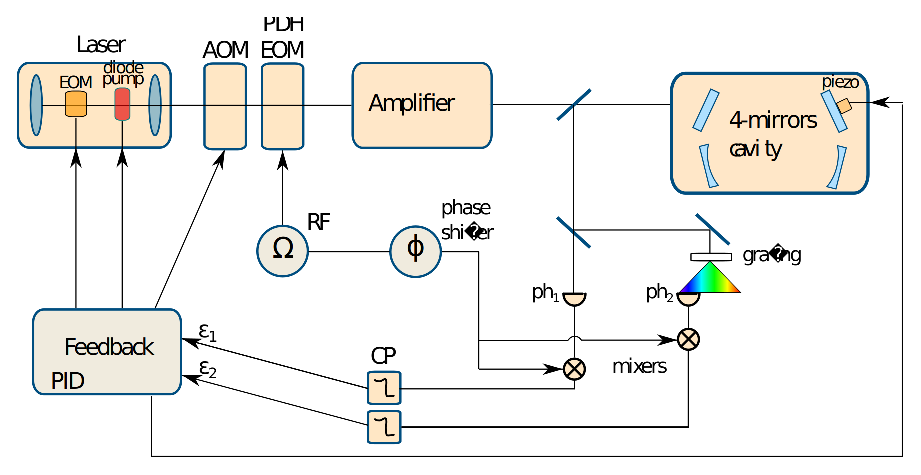
\includegraphics[width=0.9\linewidth]{images/PDH.eps}
	\caption{The double PDH system used to stabilize the cavity against the laser oscillator.}
	\label{fig:PDH}
\end{figure}
	\chapter{Theoretical concepts}

Having talked about the MariX project and explained the motivation behind the development of a dual-color X-rays source, in this chapter I will explore the theoretical background needed to understand the experimental results obtained during the thesis work.
The first part of the chapter is dedicated to explaining the inverse Compton scattering process, while in the second broader part I will talk about optical resonators theory and its application to our Fabry-Perot cavities.

\section{The inverse Compton scattering process}
\subsection{Direct Compton and Thomson scattering}
Compton scattering was observed and explained by Arthur Holly Compton in 1923 \parencite{Compton1923}, the discovery earned him the 1927 Nobel Prize in Physics. The process consists in the scattering of a photon by a charged particle like an electron, in the interaction the static electron gains momentum while the photon loses energy and changes direction. The situation is represented in Fig \ref{fig:compton}. The effect was observed by sending X-rays against a graphite target, the published results demonstrated that light can't be fully described by a classical wave theory.
\begin{figure}
	\centering
	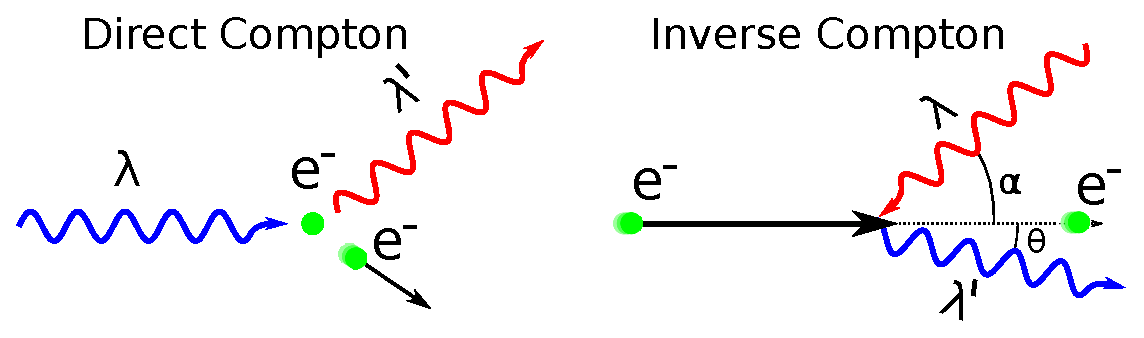
\includegraphics[width=0.9\linewidth]{images/compton.eps}
	\caption{On the left: Direct Compton scattering, the photon loses energy and the electron accelerates, the wavelength increases.
	On the right: Inverse Compton scattering, the photon recoils on the relativistic electron and gains energy proportional to the Lorentz factor squared $\gamma^2$, the wavelength decreases.}
	\label{fig:compton}
\end{figure}

In some occasions the interaction can be treated in the classical limit, in which case it is called Thomson scattering. Thomson scattering doesn't account for the change in wavelength of the incident light but represents a very good approximation when the photon frequency is low, in particular when $h\nu \ll m_e c^2$ is true.

We can describe the incident field as:
\begin{align}
\vec{E_i}= \hat{\epsilon} E_0 e^{i(\vec{k} \cdot \vec{x}-\omega t)}
\end{align}
where $ \hat{\epsilon}$ is the polarization versor. This field will displace the electron at position $\vec{x}_0$ by a small amount $\vec{x}(t) = \vec{x}_0+\delta \vec{x}(t)$. Using Newton's second law $\vec{F}=m \delta\ddot{\vec{x}}(t)$ we write:
\begin{align}
-e\,\hat{\epsilon} E_0 e^{i(\vec{k} \cdot \vec{x}-\omega t)} = m\delta\ddot{\vec{x}}(t)
\label{eq:newton}
\end{align}
In the Thomson limit we can use the approximation $\left|\delta\vec{x}\right| \ll \lambda$ to write $e^{i(\vec{k} \cdot \vec{x})} \approx e^{i(\vec{k} \cdot \vec{x}_0)}$. Solving then the differential equation \ref{eq:newton} yields
\begin{align}
\delta \vec{x}(t) = \frac{eE_0 e^{i(\vec{k} \cdot \vec{x}_0-\omega t)}}{m \omega^2} \hat{\epsilon}
\end{align}
The scattered light corresponds to the radiation emitted by the oscillating dipole $\vec{P}=-e\,\delta \vec{x}$, using the dipole emission formula \parencite{jackson_classical_1999} we can calculate the far field scattered emission at a distance $R$ from the source
\begin{equation}
\vec{E_s} = -\frac{k^2}{R} \,\hat{n} \times (\hat{n} \times \vec{P}) \,e^{ikR}
\end{equation}
The scattered light is polarized and has the same wavelength as the original light. An interesting quantity that can be calculated is the Thomson cross-section, which is $\sigma_T \approx 6.652 \times 10^{-29}\,\mathrm{m}^2$ (from \parencite{jackson_classical_1999}).

If the light is composed of high energy photons the classical approximation doesn't hold anymore, as the photons experience a change in wavelength due to the energy transfer with the electrons. In this case we need to describe light as comprised of photons with momentum
\begin{align}
\left|\vec{p_p}\right| = \frac{h\nu}{c} = \frac{h}{\lambda}
\end{align}
and energy
\begin{align}
E_p = p_p c = \frac{hc}{\lambda}
\end{align}
We consider a stationary electron, with energy equal to the rest energy $E_e = m c^2$ and momentum zero.
After the collision, the photon will have momentum  $\vec{p_p}'$ and energy $E_p'$.
Conservation of energy and momentum implies:
\begin{align}
E_p + m c^2 = E_p' + E_e' \\
\vec{p_p} = \vec{p_p}' + \vec{p_e}'
\end{align}
After some algebraic manipulation of these two equations, one obtains
\begin{align}
\frac{1}{p_f'}-\frac{1}{p_f} = \frac{1}{m c} \left( 1-\cos\theta\right)
\end{align}
where $\theta$ is the angle between $\vec{p_f}'$ and $\vec{p_f}$, that is the angle at which the photon is scattered. The Compton shift is then:
\begin{align}
\lambda'-\lambda = \frac{h}{m c} \left( 1-\cos\theta\right)
\end{align}
The maximum change in photon wavelength occurs when $\theta = 180\degree$, in this case the process is called Compton back-scattering.

\subsection{Inverse Compton scattering}
Direct Compton scattering deals with the case of a photon losing energy to an electron, when the opposite is true the process is called Inverse Compton Scattering. ICS occurs when photons are scattered by relativistic electrons ($v\sim c$), in this case the light is upshifted in frequency by a factor determined by the electrons velocity and proportional to $\gamma^2$, where $\gamma$ is the Lorentz factor. 
By making use of the principle of relativity we can describe the interaction in the electron rest frame and use the obtained results for direct Compton scattering, then return to the ``lab'' frame of reference using a Lorentz boost.

In the lab frame, the photon has frequency $\nu$ and is approaching the electron at an angle $\alpha$, the electron has relativistic velocity $\beta$, corresponding to the Lorentz factor $\gamma = 1/\sqrt{1-\beta^2}$. After the collision the photon will leave the interaction point at an angle $\theta$ with frequency $\nu_s$. The situation is represented in Fig \ref{fig:compton}.

We can calculate the photon frequency $\nu'$ in the electron rest frame using Lorentz transformations and remembering that $\vec{k} \cdot \vec{x}-\omega t$ is invariant under such transformations, we get:
\begin{align}
\nu' = \nu \gamma \left( 1+\beta \cos\alpha\right)
\end{align}
Since in BriXS the maximum energy reached by the electrons will be about 100\,MeV, corresponding to $\gamma \approx 200$, we can verify that in their rest frame the scattering occurs in the Thomson limit ($h \nu' \ll mc^2$):
\begin{align*}
h \nu' < 2 \gamma h \nu \approx 480\,eV && mc^2 \approx 5 \times 10^5\,eV
\end{align*}
In this limit the scattered light doesn't change frequency:
\begin{align}
\nu_s' = \nu'
\end{align}
but it changes direction, if we consider the light coming out at an angle $\theta'$ and then shift back to the lab frame via a second Lorentz boost we obtain:
\begin{align}
\nu_s = \nu_s' \gamma \left( 1-\beta \cos\theta'\right)
\end{align}
where
\begin{align}
\cos \theta' = \frac{\cos\theta -\beta}{1-\beta\cos\theta}
\end{align}
Substituting in the last expression we arrive at the final result, relating the scattering angles and the electron energy with the final photon energy:
\begin{align}
\nu_s = \nu\frac{1+\beta\cos\alpha}{1-\beta\cos\theta} \approx \nu\frac{2\gamma^2\left( 1+\cos\alpha\right)}{1+\gamma^2\theta^2}
\label{eq:ICS}
\end{align}
where the last approximation holds for $\theta\ll 1$. In practice, because of the second Lorentz boost, almost all the radiation is confined in an angle $\theta_m \approx 1/\gamma$ so the approximation is very accurate. Maximum emission and photon energy is reached for $\theta = 0$, varying the acceptance angle one can control the bandwidth of the extracted radiation \parencite{Drebot2017}, as showed in Fig \ref{fig:ics}.
\begin{figure}
	\centering
	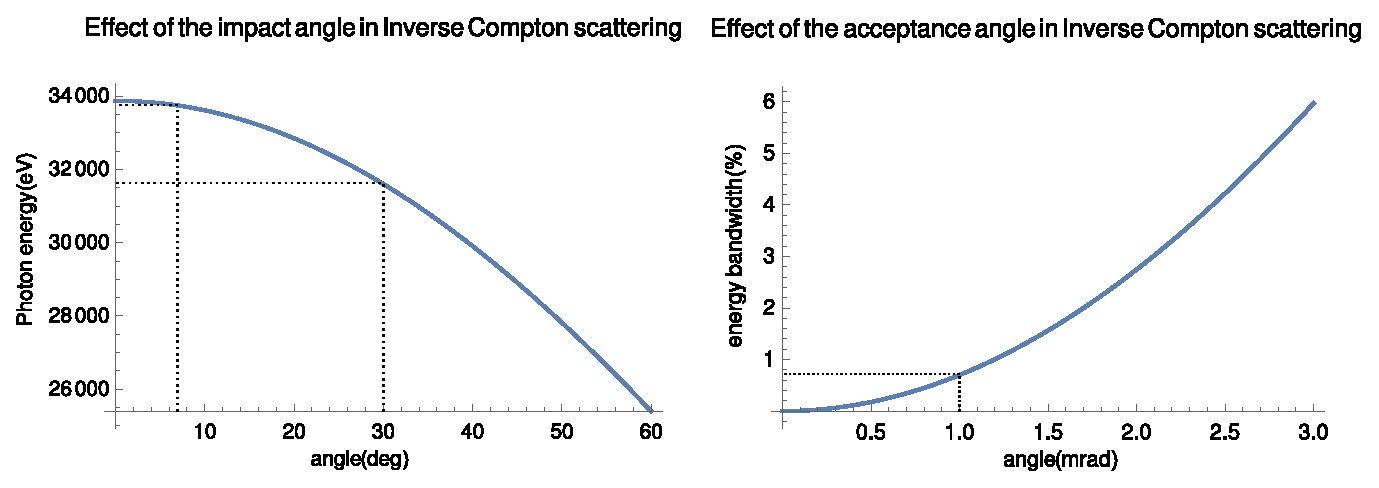
\includegraphics[width=1\linewidth]{images/ics.eps}
	\caption{Effect of the impact angle and of the acceptance angle in ICS: we can see that two cavities placed at $7\degree$ and $30\degree$ with respect to the electron beam produce the energies needed for iodine KES. BriXS will have a tunable bandwidth of $\Delta E/E \sim 1-10\%$, for KES the bandwidth must be kept low in order to achieve reasonable separation between the two colors, so a small acceptance angle ($\theta \approx 1$\,mrad) is preferred.}
	\label{fig:ics}
\end{figure}
Following \ref{eq:ICS} we can calculate the electron energy needed to reach the iodine K-edge, that is to produce X-rays with energy $h \nu_s \approx 34$\,keV in our first cavity. Given the geometry of the cavity and the mirror size the angle at the interaction point will be 7\degree, while
\begin{align}
\gamma = \sqrt{\frac{\nu_s}{\nu}\frac{1}{2(1+\cos 7 \degree)}} \approx 84
\end{align}
corresponding to an energy $E_e \approx$ 42\,Mev.
The second cavity will need to produce X-rays below the iodine edge, at 32\,keV. From the Fig \ref{fig:ics} we see that this is doable for an interaction angle of 30\degree. This means that the two crossed Fabry-Perot cavities will have to be placed with an angle of $23\degree$ between each other.

Different angles means also that the laser pulses interact with the electron bunches differently in the two cavity, in particular the time during which the pulses and the bunches overlap varies, this results in different luminosity for the two colors. Following \parencite{Variola2011} we can write the number of interaction per second in the Compton process as:
\begin{align}
N = \sigma_T f_\mathrm{rep} N_{ph} N_e G
\end{align}
where $G$ is the ``geometric factor'' and corresponds to the space-time interval in which the pulses and bunches overlap, $N_e$ and $N_{ph}$ are the electron and photon numerical densities, $f_\mathrm{rep}$ is the number of pulses interacting per second (equal to the repetition rate of the laser oscillator) and $\sigma_T$ the Thomson cross-section. Assuming a tri-gaussian shape for both, the rate of the scattering process is:
\begin{align}
N = \frac{\sigma_T f_\mathrm{rep} N_{ph} N_e}{2\pi\sqrt{\sigma_{Ly}^2+\sigma_{y}^2}\sqrt{\sigma_{Lx}^2+\sigma_{x}^2+\left(\sigma_{Lz}^2+\sigma_{z}^2\right)\tan^2(\frac{\alpha}{2})}}
\label{eq:N}
\end{align}
where the L subscript identifies the laser pulse dimensions as opposed to the electron bunch dimensions. To achieve the same luminosity for both the colors we can change the laser pulse dimension ($\sigma_{Ly}$ and $\sigma_{Lx}$) at the IP, compensating the $\sqrt{\tan^2(\alpha/2)}$ factor at the denominator.

Possible electron bunch and laser spot sizes are shown in Table \ref{tab:size}.
\begin{figure}
	\centering
	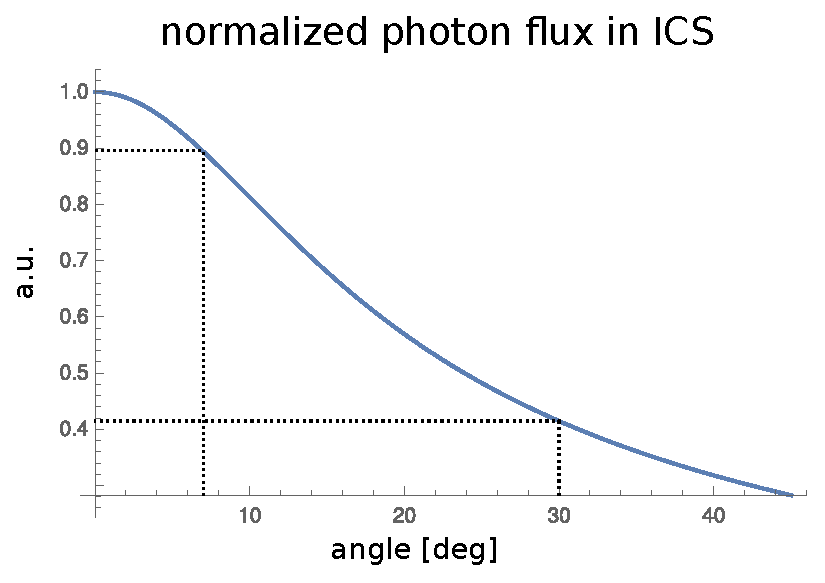
\includegraphics[width=0.9\linewidth]{images/photonflux.eps}
	\caption{Normalized photon flux in Inverse Compton Scattering as a function of the angle between the laser and the electron bunch. The values for the electron bunch and laser pulse size are that of the first two columns of \ref{tab:size}. Without changing the pulse size in the two cavities the flux would differ by a factor $\approx 2$.}
	\label{fig:photonflux}
\end{figure}
\begin{table}
	\centering
\begin{tabular}{|c|c|c|c|}
	\hline 
	&e$^- bunch$  &Laser $\alpha=7\degree$  &Laser $\alpha=30\degree$  \\ 
	\hline 
$\sigma_x [\mathrm{\mu m}] $	& 25 & 60 & 24 \\ 
	\hline 
$\sigma_y [\mathrm{\mu m}]$	& 15 & 40 & 15 \\ 
	\hline 
$\sigma_z [\mathrm{\mu m}]$  & 440 & 300 & 300 \\
	\hline

\end{tabular}
	\caption{Possible values for the electron bunches and laser pulses dimensions, this configuration gives the same luminosity for the two colors produced at different angles.}
\label{tab:size}
\end{table}

From \ref{eq:N}, and its dependence from the low Compton cross-section\\ ($\sigma_T=6.652\times 10^{-29}$\,m$^{-2}$) it is clear that a high photon flux is required to reach efficient generation of X-rays, hence the need for power enhancing Fabry-Perot optical cavities.

\section{Optical cavities}
\begin{figure}
	\centering
	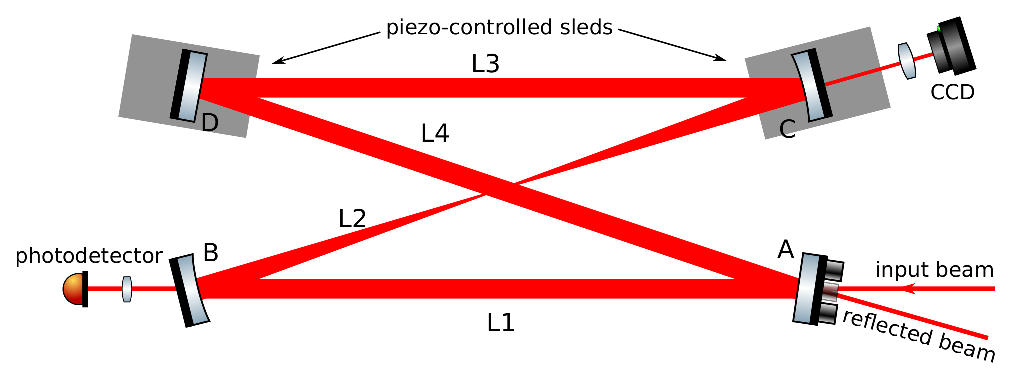
\includegraphics[width=1\linewidth]{images/cavity.eps}
	\caption{The 4-mirror confocal bow-tie cavity design. Mirror A is the input coupler and it is mounted on the piezoelectric ring crystal used by the PDH system to stabilize the cavity. B and C are the curved mirrors, they are mounted on a computer-controlled positioning system able to change their orientation, and in doing so move the cavity waist. Mirror C and D are mounted on two sleds used to adjust the cavity length, by moving both at the same time it is possible to change the distance between the curved mirrors while maintaining the cavity length. The reflected beam is used by the PDH system to create the error signal needed for the stabilization.}
	\label{fig:cavity}
\end{figure}

A resonant optical cavity consists of multiple optical elements that force light to travel in a closed path. The simplest such arrangement is two mirrors facing each other. A Fabry-Perot cavity is a passive optical resonator (i.e. without gain medium) in which only particular frequencies can be coupled (through an input coupler) and transmitted through the other mirrors, while other frequencies are reflected.
The optical power in the resonator is enhanced by a factor that depends on the cavity losses and the input coupling efficiency, those are determined mainly by the cavity mirrors reflectivity.

The proposed cavity design for BriXS, and the one developed in our laboratory, is a 4-mirror confocal bow-tie cavity. As we will see, a confocal cavity is very stable against the misalignment of optical elements, this is useful since our objective is to move the cavity focus in and out of the interaction point by deliberately misaligning the curved mirrors in the vertical direction, and in doing that we don't want to change the coupling with the external laser source or the resonating frequency. The cavity design is represented in Fig \ref{fig:cavity}.

\subsection{Ray optics and the ABCD matrix formalism}

To better understand the propagation of light waves inside a resonator we start by introducing the ABCD matrix formalism for optical ray propagation \parencite{Brouwer1964,siegman86}. We will also use this theoretical tool to make predictions on the behavior of the laser beam and waist inside the cavity.
\begin{figure}
	\centering
	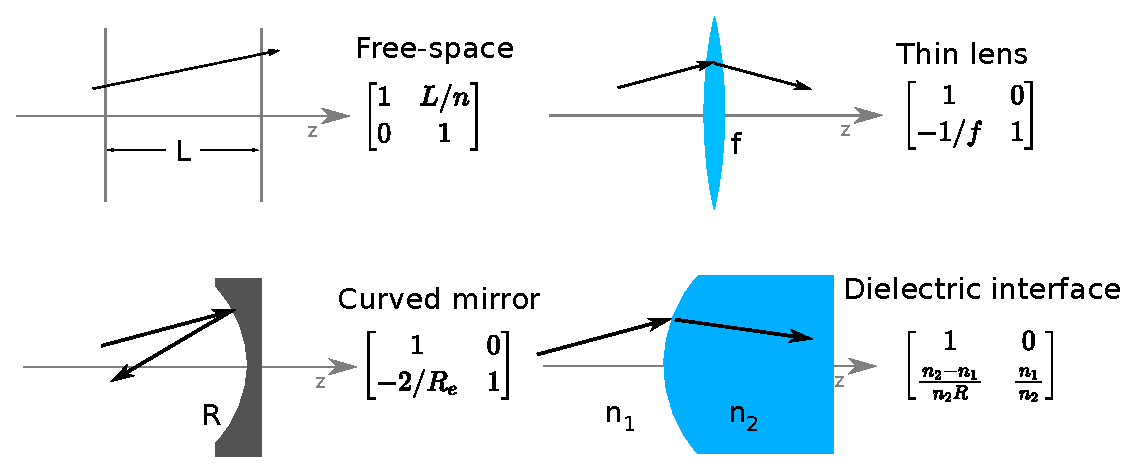
\includegraphics[width=1\linewidth]{images/abcd.eps}
	\caption{ABCD matrices for various paraxial optical elements. In the case of the curved mirror, $R_e$ is the ``effective radius'' for non normal incidence, equal to $R/\cos\theta$ for the vertical direction and $R\cos\theta$ in the horizontal direction, where $\theta$ is the angle of incidence. A curved mirror is an astigmatic element.}
	\label{fig:abcd}
\end{figure}

Let's consider a light ray traveling roughly in the $z$ direction, at a distance $r(z)$ from the reference $z$ axis and with a small inclination $r'=dr/dz$: if it travels from  location $z_1$ to $z_2$ for a length $L$, the distance and inclination $r_2$ and $r'_2$ in $z_2$ will be:
\begin{align}
r_2 &= r_1 + \frac{L}{n}\frac{dr_1}{dz} = r_1 + \frac{L}{n}r'_1  \\
r'_2 &= \frac{dr_2}{dz} = r'_1
\end{align}
where $n$ is the refractive index of the medium.
If the ray goes through a converging thin lens with focal distance $f$, its $r$ and $r'$ parameters immediately before and after the lens will be related by:
\begin{align}
r_2 &= r_1 \\
r'_2 &= -\frac{1}{f}r_1 +r'_1
\end{align}
Obviously the ray does not change its distance from the optical axis, but the slope changes because of the lens focusing power.
In both these cases a linear transformation relates the properties of the ray before the optical elements with that of the ray after the element. These transformations can then be written in matrix form, with the matrix acting on the ray vector $\boldsymbol{r} = (r,r')^T$:
\begin{align}
\begin{bmatrix}
	r_2 \\
	r'_2
\end{bmatrix}
=
\begin{bmatrix}
	A & B\\
	C & D
\end{bmatrix}
\begin{bmatrix}
	r_1 \\
	r'_1
\end{bmatrix}
\end{align}
The transformation representing the thin lens for example is:
\begin{align*}
\begin{bmatrix}
r_2 \\
r'_2
\end{bmatrix}
=
\begin{bmatrix}
1 & 0\\
-1/f & 1
\end{bmatrix}
\begin{bmatrix}
r_1 \\
r'_1
\end{bmatrix}
\end{align*}
Matrices representing other paraxial optical elements are shown in Fig \ref{fig:abcd}. It is important to note that the determinant of these ABCD matrix is given by $AB-CD=n_1/n_2$, or 1 in the case of the same medium. A complex system composed of multiple optical elements $M_1,M_2,\dots$ can then be described by a single ABCD matrix obtained by matrix multiplication:
\begin{align*}
M = \dots M_3 M_2 M_1
\end{align*}
By the property of matrix multiplication, $M$ will also have unitary determinant (if the ray starts and arrives in the same medium). A consequence of this fact is that every complex ABCD system between two optical planes can be described as a thin lens ($f$) surrounded by two free space propagations ($L_1$,$L_2$): since the matrix has only three free parameters, by accurately choosing $f,L_1,L_2$ one can recreate the same ABCD values of the complex system.
\begin{figure}
	\centering
	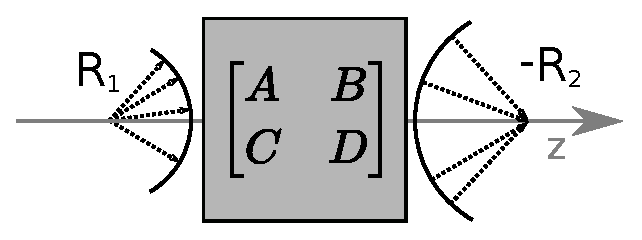
\includegraphics[width=0.9\linewidth]{images/abcdradius.eps}
	\caption{After passing through a general ABCD system, a spherical wavefront is still spherical but the radius of curvature is changed according to \ref{eq:radius}}
	\label{fig:radius}
\end{figure}

Ray matrices can also be used to describe the propagation of spherical waves: a spherical wave can be seen as a collection of rays originating from a common point but with different orientation, as shown in Fig \ref{fig:radius}. For each of these rays holds that:
\begin{align}
	r'(z) = \frac{dr}{dz} = \frac{r(z)}{R(z)}
\end{align}
where $R(z)$ is the distance from the wavefront center of curvature.
After passing through an ABCD system the wavefront radius will change following:
\begin{align}
R_2 = \frac{r_2}{r'_2} = \frac{Ar_1+Br'_1}{Cr_1+Dr'_1}= \frac{AR_1+B}{CR_1+D}
\label{eq:radius}
\end{align}
Thus, a spherical wavefront remains spherical after propagating through a paraxial optical system.

In 3D space a ray will in general be described by two displacements from the $z$ axis, in directions $x$ and $y$, if the ray passes through astigmatic elements, such as spherical mirrors with non-normal incidence, the matrices for the two directions will be different.

\subsubsection{Stability of optical resonators}
In an optical cavity the beam passes through the same optical elements (usually mirrors) over and over, if $M$ is the matrix representing the cavity, after $n$ passes the original ray $\boldmath{r_1}$ will become:
\begin{align}
\boldsymbol{r_2} = M^n \boldsymbol{r_1}
\end{align}
After an infinite number of passes the ray will either remain confined in a bounded region or diverge to infinity, in the first case the cavity is called stable, while in the other unstable.
We can study this behavior by expanding a generic ray on the cavity eigenrays, that is $\boldsymbol{r_{a,b}}$ such that:
\begin{align}
M \boldsymbol{r_{a,b}} = \lambda_{a,b} \boldsymbol{r_{a,b}}
\end{align}
A generic ray $\boldsymbol{r} = a \boldsymbol{r_{a}} + b \boldsymbol{r_{b}}$ will then evolve following:
\begin{align}
M^n \boldsymbol{r} = a \lambda_{a}^n \boldsymbol{r_{a}} + a \lambda_{b}^n \boldsymbol{r_{b}}
\end{align}
The eigenvalues can be found from $M$ via:
\begin{align}
	\begin{vmatrix}
	A-\lambda & B\\
	C & D-\lambda\\
	\end{vmatrix}
	&= \lambda^2 - (A+D)\lambda +1 = 0 \\
	\lambda_{a,b} &= m \pm \sqrt{m^2-1}
\end{align}
where $m=(A+D)/2$ is the so-called ``stability parameter'' (or ``m parameter'') for the system.
We can now see that if $-1\le m\le1$ then the two eigenvalues will be unitary conjugate complex numbers $e^{\pm i\theta}$, giving
\begin{align}
M^n \boldsymbol{r} = a e^{i\theta n} \boldsymbol{r_{a}} + b e^{-i\theta n} \boldsymbol{r_{b}} = \boldsymbol{s_1} \cos\theta n + \boldsymbol{s_2} \sin\theta n
\end{align}
The ray will remain confined in an area determined by the initial condition, the cavity in this case is stable.
If $|m|>1$ the two eigenvalues will be real and the ray will evolve according to:
\begin{align}
	M^n \boldsymbol{r} = \boldsymbol{s_1} \cosh\theta n + \boldsymbol{s_2} \sinh\theta n
\end{align} 
meaning that its propagation is unbound, the cavity is unstable.
\begin{figure}
	\centering
	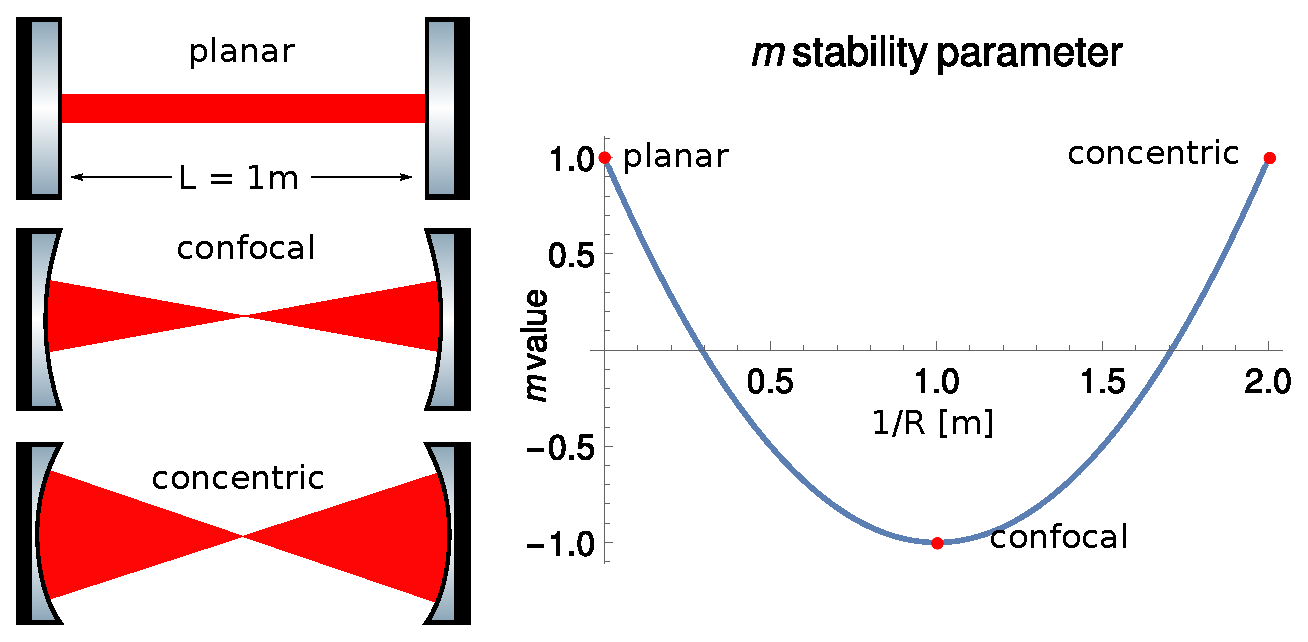
\includegraphics[width=1\linewidth]{images/mstability.eps}
	\caption{Three type of resonators: the planar and concentric cavities have $m=1$ while the confocal cavity has $m=-1$, they all are on the edge of stability. From the plot it is clear that a near-confocal cavity is stable while a near-concentric or near-confocal can have $m>1$.}
	\label{fig:mstability}
\end{figure}

Having explained the importance of the stability parameter, let's use it to determine the stability of various cavity types. In Fig \ref{fig:mstability} three different cavities composed by two curved mirrors are represented, their ABCD matrix representation can be obtained multiplying the matrices for the two mirrors and two free space propagations. We are interested in the stability parameter, if $R_1$ and $R_2$ are the radii of the mirrors and $L$ the distance between them $m$ is:
\begin{equation}
m = 2\left( 1- \frac{L}{R_1} \right)\left( 1- \frac{L}{R_2} \right)-1
\end{equation}
We can see in Fig \ref{fig:mstability} that confocal, concentric and planar resonators are on the ``stability edge''; however, small deviations in $L$, $R1$ or $R2$ can make a concentric or planar resonator unstable, while a confocal resonator remains stable.

\subsubsection{The 3x3 Matrix formalism for misaligned elements}

Until now we have considered optical elements perfectly placed and oriented on an imaginary optical axis, from which the ray parameters $r$ and $r'$ are calculated.
We can now study how a misaligned optical element acts on a light ray. A misaligned optical element acts with the same ABCD matrix but on an axis (called ``element axis'') different from the reference optical axis. The situation is represented in Fig \ref{fig:misaligned}.
\begin{figure}
	\centering
	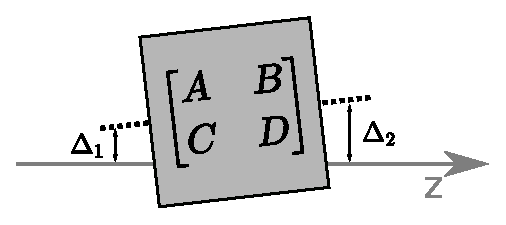
\includegraphics[width=1\linewidth]{images/misaligned.eps}
	\caption{A misaligned optical element: its axis does not match the reference optical axis $z$.}
	\label{fig:misaligned}
\end{figure}
Let's consider an optical ABCD element of length $L$ shifted by $\Delta_1$ from the optical axis at the input plane and $\Delta_2$ at the output plane, its slope in respect to the reference is 
\begin{align}
\Delta' = \frac{\Delta_2-\Delta_1}{L}
\label{eq:delta}
\end{align}
Assuming no changes happen in the refractive index, the slope is the same at the input and output planes.
The \ref{eq:delta} can also be written
\begin{align}
\boldsymbol{\Delta_2}=
\begin{bmatrix}
\Delta_2 \\
\Delta'
\end{bmatrix}
=
\begin{bmatrix}
1 & L \\
0 & 1 \\
\end{bmatrix}
\begin{bmatrix}
\Delta_1 \\
\Delta'
\end{bmatrix}
=M_\Delta \boldsymbol{\Delta_1}
\end{align}

A ray characterized by parameters $r_1$ and $r'_1$ will be represented on the element axis by
\begin{align}
s_1 = r_1 - \Delta_1 && s'_1 = r'_1 - \Delta'
\end{align}
We know how the element acts on $\boldsymbol{s_1}$:
\begin{align}
\boldsymbol{s_2} =
\begin{bmatrix}
s_2 \\
s'_2
\end{bmatrix}
=
\begin{bmatrix}
A & B \\
C & D \\
\end{bmatrix}
\begin{bmatrix}
s_1 \\
s_1'
\end{bmatrix}
=M \boldsymbol{s_1}
\end{align}
Returning to the reference axis we get the overall effect of the misaligned element:
\begin{align}
\boldsymbol{r_2} &= \boldsymbol{s_2} + \boldsymbol{\Delta_2}\\
\boldsymbol{r_2} = M\boldsymbol{s_1} + M_\Delta \boldsymbol{\Delta_1} &= M\boldsymbol{r_1} + (M_\Delta - M)\boldsymbol{\Delta_1} = M\boldsymbol{r_1} + \boldsymbol{E}
\end{align}
The misaligned element acts like its aligned counterpart except for the addition of an ``error vector'' $\boldsymbol{E}$ to the optical ray.
The total transformation $M\boldsymbol{r_1}+\boldsymbol{E}$ can be represented on a 3x3 matrix:
\begin{align}
\begin{bmatrix}
r_2 \\
r'_2 \\
1
\end{bmatrix}
=
\begin{bmatrix}
A & B & E\\
C & D & F\\
0 & 0 & 1
\end{bmatrix}
\begin{bmatrix}
r_1 \\
r_1'\\
1
\end{bmatrix}
\label{eq:abcdef}
\end{align}
\begin{align}
E = (1-A)\Delta_1 + (L-B)\Delta' && F = -C\Delta_1 + (1-D)\Delta'
\end{align}
This representation is very useful because it permits to easily calculate the overall matrix of a complex system of misaligned elements, such as a cavity with misaligned mirrors, via matrix multiplication.

If we consider a resonator and its ABCDEF round-trip matrix we can see that a ray lying on the reference optical axis $\boldsymbol{r} = (0,0,1)^T$ will in general not superimpose with itself after a round-trip of the cavity:
\begin{align}
\begin{bmatrix}
A & B & E\\
C & D & F\\
0 & 0 & 1
\end{bmatrix}
\begin{bmatrix}
0 \\
0\\
1
\end{bmatrix}
=
\begin{bmatrix}
E \\
F \\
1
\end{bmatrix}
\end{align}
To find the overall ``axis ray'' of the cavity, that is the ray that after a round-trip of the cavity has the exact same position and slope, one must solve the ``eigenray'' problem:
\begin{align}
M \boldsymbol{r_0} = \boldsymbol{r_0}
\end{align}
The solution is:
\begin{align}
r_0 = \frac{(1-D)E + BF}{2-A-D} && r_0' = \frac{CE + (1-A)F}{2-A-D}
\label{eq:eigenray}
\end{align}
This is the resonating ray of the cavity, all other rays will behave according to the results of the previous section on stable and unstable resonators in reference to this axis ray. In particular a ray $\boldsymbol{r_1}$ after a round-trip will evolve following:
\begin{align}
\boldsymbol{r_2}-\boldsymbol{r_0} = M_{2\times2} (\boldsymbol{r_1}-\boldsymbol{r_0})
\end{align}
To efficiently couple a Fabry-Perot cavity with an external ray, matching between the external ray and the axis ray is required.
It is important to note that for a near planar or near concentric cavity $A+D \approx 2$, according to \ref{eq:eigenray} this means that the cavity is extremely unstable regarding misalignment, while for a near confocal cavity $A+D \approx -2$ giving maximum stability.

\subsubsection{Cavity focus movement through moving mirrors}
We can now apply this formalism to our crossed cavities and verify that we can move the ray resonating in the cavity, and in particular the location of the beam waist between the curved mirrors, by accurately tilting the curved mirrors.

Since the objective is to use this movement to vertically move the focus of one cavity in and out of the interaction point with the electrons, we need to calculate the round-trip matrix for the vertical direction. The ABCDEF matrix for the plane mirrors is simply the identity matrix\footnote{We don't consider ray inversion\parencite{siegman86,Plachenov2011} since our cavity has an even number of mirrors.}, while that of the tilting curved mirrors is :
\begin{align}
M_{b,c}(d\alpha) = 
\begin{bmatrix}
1 & 0 & 0\\
-2\frac{\cos\theta/2}{R_{b,c}} & 1 & 2d\alpha\\
0 & 0 & 1
\end{bmatrix}
\end{align} 
where $d\alpha$ is the tilt angle, $\theta/2$ the angle of incidence on the mirror and $R_{b,c}$ the mirror radius of curvature (in our case $\theta/2 = 7\degree /2 = 3.5\degree$ and $R_b=R_c=750$\,mm).
The free space propagation matrix has the expression:
\begin{align}
M_L = 
\begin{bmatrix}
1 & L & 0\\
0 & 1 & 0\\
0 & 0 & 1
\end{bmatrix}
\end{align}
The overall cavity matrix calculated from the focus plane is then:
\begin{align}
\begin{split}
M = 
\begin{bmatrix}
1 & L_2/2 & 0\\
0 & 1 & 0\\
0 & 0 & 1
\end{bmatrix}
\begin{bmatrix}
1 & 0 & 0\\
-2\frac{\cos\theta/2}{R_{b}} & 1 & 2d\alpha\\
0 & 0 & 1
\end{bmatrix}
\begin{bmatrix}
1 & L_1 & 0\\
0 & 1 & 0\\
0 & 0 & 1
\end{bmatrix}
\begin{bmatrix}
1 & L_4 & 0\\
0 & 1 & 0\\
0 & 0 & 1
\end{bmatrix}\\
\begin{bmatrix}
1 & L_3 & 0\\
0 & 1 & 0\\
0 & 0 & 1
\end{bmatrix}
\begin{bmatrix}
1 & 0 & 0\\
-2\frac{\cos\theta/2}{R_{c}} & 1 & 2d\alpha\\
0 & 0 & 1
\end{bmatrix}
\begin{bmatrix}
1 & L_2/2 & 0\\
0 & 1 & 0\\
0 & 0 & 1
\end{bmatrix}
\end{split}
\end{align}
\begin{figure}
	\centering
	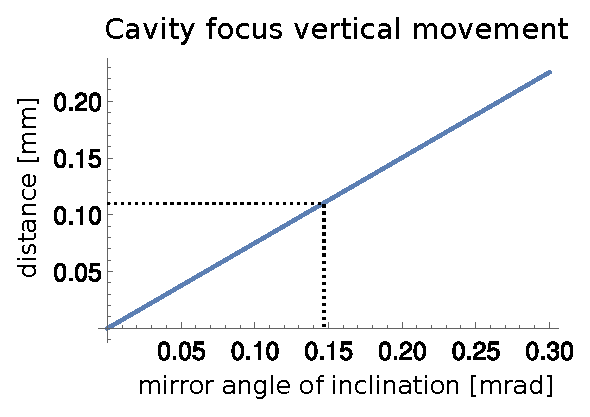
\includegraphics[width=0.8\linewidth]{images/shiftfocus.eps}
	\caption{Focus vertical movement versus angular misalignment of mirrors B and C, to reach $110\,\mu$m of movement we need to tilt the mirrors for about $150\,\mu$rad.}
	\label{fig:shiftfocus}
\end{figure}
where the lengths $L_i$ are distances between the mirrors labeled in Fig \ref{fig:cavity}. 
The focus vertical movement $r_0(d\alpha)$ is then given by \ref{eq:eigenray}, the results are shown in Fig \ref{fig:shiftfocus}.
If we consider the possible spot sizes given in Tab \ref{tab:size} we can see that to switch between the two cavities we need a movement of at least $w_{1y}+w_{2y}=2(\sigma_{1y}+\sigma_{2y})\approx 110\,\mu$m, corresponding to a mirror inclination of about $150\,\mu$rad.

The cavity length is unaffected by the mirror movement if the rotation pivot is at the same height as the laser beam. However our mirrors rotate around an axis situated about $r =16$\,mm under the laser beam height, that means that during the rotation the mirror moves forward. The cavity length would be reduced by
\begin{align}
	\delta L = \frac{4 r d\alpha }{\cos 3.5\degree}
\end{align}
which amounts to about $10\,\mu$m for the desired movement, just beyond the limit of our current stabilization system. To eliminate this problem, new mirror mounting with gimbal-like movement are being developed in our laboratory.

\subsection{Longitudinal and transverse modes}

Light propagation inside a cavity can be described using Huygens integral, considering each point as a spherical wave source, and the paraxial approximation. Given an electric field distribution $E_0(x_0,y_0,z_0)$ (we assume sinusoidal time dependence) Huygens integral allows us to calculate the field in a generic point via:
\begin{align}
\begin{split}
&E(x,y,z) =\\ &\frac{i}{\lambda}\frac{e^{-ik(z-z_0)}}{z-z_0}\iint E_0(x_0,y_0,z_0) \exp\left[-ik\frac{(x-x_0)^2+(y-y_0)^2}{2(z-z_0)}\right]\mathop{dx_0}\mathop{dy_0}
\end{split}
\label{eq:huygens}
\end{align}
where $(z-z_0)^2\gg(x-x_0)^2+(y-y_0)^2$ for the validity of the paraxial (or ``Fresnel'') approximation.
This is true for free-space propagation, however if the field goes through an ABCD optical system (like an optical cavity) eq. \ref{eq:huygens} becomes \parencite{svelto2010}:
\begin{align}
\begin{split}
&E(x,y,z) =\\ &\frac{i}{\lambda}\frac{e^{-ikB}}{B}\iint E_0 \exp\left[-ik\frac{A(x_0^2+y_0^2)+D(x^2+y^2)-2(xx_0+yy_0)}{2B}\right]\mathop{dx_0}\mathop{dy_0}
\end{split}
\label{eq:huy2}
\end{align}
By substitution it can be verified that functions of the form:
\begin{align}
f_0(x,y) \propto \exp\left[-ik\frac{x^2+y^2}{2q_0}\right]
\label{eq:gauss}
\end{align}
where $q_0$ is a complex parameter (we ignored the longitudinal phase-shift $\exp -ik(z-z_0)$\,), are ``eigensolutions'' of \ref{eq:huy2}, if substituted in the integral one gets:
\begin{align}
f(x,y) \propto \frac{1}{A+B/q_0} \exp\left[-ik\frac{x^2+y^2}{2q}\right]
\end{align}
where $q$ is given by:
\begin{align}
	q = \frac{Aq_0+B}{Cq_0+D}
	\label{eq:q}
\end{align}
A field described by \ref{eq:gauss} is called gaussian beam, while $q$ is called the complex beam parameter. The transformation of $q$ through an optical element is similar to that of the radius of spherical wavefront, in fact if $q$ is real the gaussian beam field becomes a spherical wave field. The imaginary part of $q$ gives the transverse width of the beam, this is clear by separating $1/q$ in its real and imaginary part:
\begin{align}
	\frac{1}{q} = \frac{1}{R} -i \frac{\lambda}{\pi w^2}
\end{align}
and substituting in the gaussian beam field expression
\begin{align}
f(x,y) \propto \exp\left[-\frac{x^2+y^2}{w^2}\right] \exp\left[-ik\frac{x^2+y^2}{2R}\right]
\end{align}

The gaussian beam is not the only eigensolution of the Huygens integral, other solutions are given by the Hermite-Gauss modes:
\begin{align}
HG_{nm}(x,y)  \propto H_n\left(\frac{\sqrt{2}x}{w}\right)H_m\left(\frac{\sqrt{2}y}{w}\right)\exp\left[-ik\frac{x^2+y^2}{2q}\right]
\label{eq:HG}
\end{align}
where $H_l$ are the Hermite polynomials. These modes are orthogonal to each other and form a complete system for the electric field, they also include the gaussian beam as the lowest order mode $HG_{00}$. In an astigmatic system $q_x$ and $q_y$ will in general be different.

For a mode $E_0$ to resonate in a cavity it is not enough to retain its transverse shape after a round trip, it must also return with the same phase, that means that the mode ``eigenvalue'' $\sigma$ given by:
\begin{align}
E_{rt}(x,y,z) = \sigma E_0(x,y,z)
\end{align}
must be real. This translates to a condition on the Hermite-Gauss mode frequencies inside the resonator \parencite{siegman86}:
\begin{align}
	\nu_{lmn} = \nu_{\mathrm{FSR}}\left(l+\frac{n+1/2}{2\pi}\arccos(m_H)+\frac{m+1/2}{2\pi}\arccos(m_V)\right) 
\end{align}
Where $m_H$ and $m_V$ are the two stability parameters for an astigmatic cavity.
The mode eigenvalue $\sigma$, in addition to determining if a mode is resonant, gives the diffraction power losses of the mode after a round-trip via:
\begin{align}
	\gamma = 1- |\sigma|^2
\end{align}
\begin{figure}
	\centering
	\includegraphics[width=1\linewidth]{images/modi.png}
	\caption{Two resonant modes observed in our cavity, in the left picture the $HG_{21}$ while in the right the fundamental mode $HG_{00}$.}
	\label{fig:modi}
\end{figure}

The $HG$ modes are only approximations (albeit good) of the modes inside a real resonator, real cavity modes are subject to diffractive effects (for example due to finite mirror size) and other non-idealities. An example of modes resonating in our Fabry-Perot cavities is shown in Fig \ref{fig:modi}, for our application (inverse Compton scattering) the cavities must be stabilized to resonate only with the lowest order $HG_{00}$ mode.

To excite a mode inside the cavity, mode matching between the laser external mode and the cavity is necessary. This means that the laser oscillator output must be single-mode ($HG_{00}$) and that the $q$ parameter must be controlled, this can be achieved by a telescopic system outside the cavity. The external mode must also lie on the ``axis ray'' of the cavity (defined in the previous section), however, during the curved mirror movement, the axis ray changes. The ray parallel shift is given by $r_0$ in \ref{eq:eigenray} (the change in the angle $r_0'$ is effectively 0). To estimate the change in coupling efficiency between the two modes we can then use the overlap integral of the modes at the input coupler:
\begin{align}
	\eta(r_0) = \int H_{00}^\mathrm{cav*}(x,y-r_0)H_{00}^\mathrm{ext}(x,y)\mathop{dx}\mathop{dy} 
	\label{eq:eta}
\end{align} 
The results shown in Fig \ref{fig:couplingeta} indicate that the change in coupling efficiency is very small ($<0.5\%$).
\begin{figure}
	\centering
	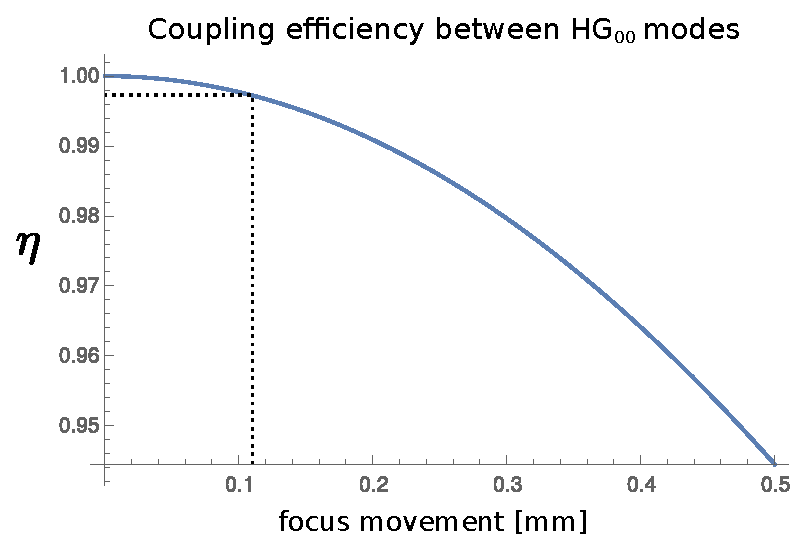
\includegraphics[width=0.8\linewidth]{images/couplingeta.eps}
	\caption{Coupling efficiency between two gaussian beams. The beam radius is set at $1.48\,$mm, as it is in our cavity. For a focus movement of $110\,\mu$m the efficiency remains over 99.5\%.}
	\label{fig:couplingeta}
\end{figure}

\subsection{Cavity Finesse and enhancement of the optical power}
\begin{figure}
	\centering
	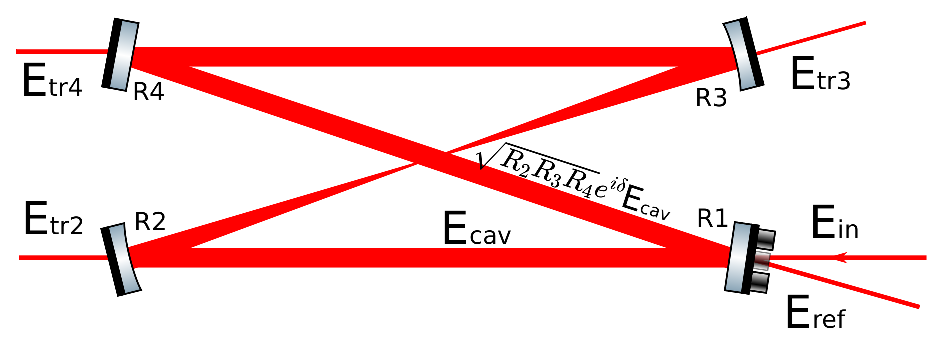
\includegraphics[width=0.9\linewidth]{images/ecav.eps}
	\caption{Electric fields inside the cavity. A full round trip of the cavity carries a phase factor $e^{i\delta}$ and a reflection on the input mirror causes a phase shift of $\pi$.}
	\label{fig:ecav}
\end{figure}
\begin{figure}
	\centering
	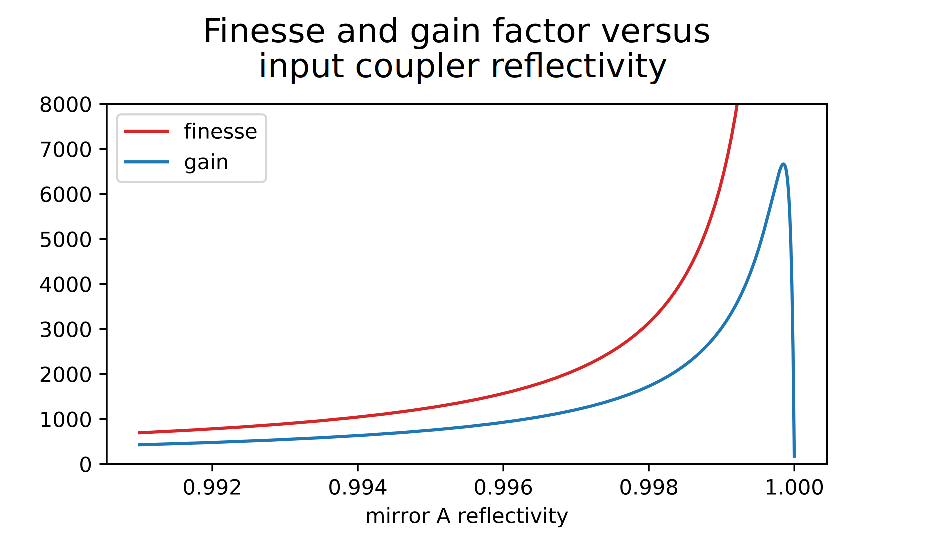
\includegraphics[width=0.9\linewidth]{images/finessegain.eps}
	\caption{Finesse and gain of a 4-mirror Fabry-Perot cavity. The reflectivities of mirror B, C and D are set to 0.99995. When the input coupler (mirror A) transmission is high the $a$ factor goes to $\pi/2$.}
	\label{fig:finessegain}
\end{figure}
\begin{figure}
	\centering
	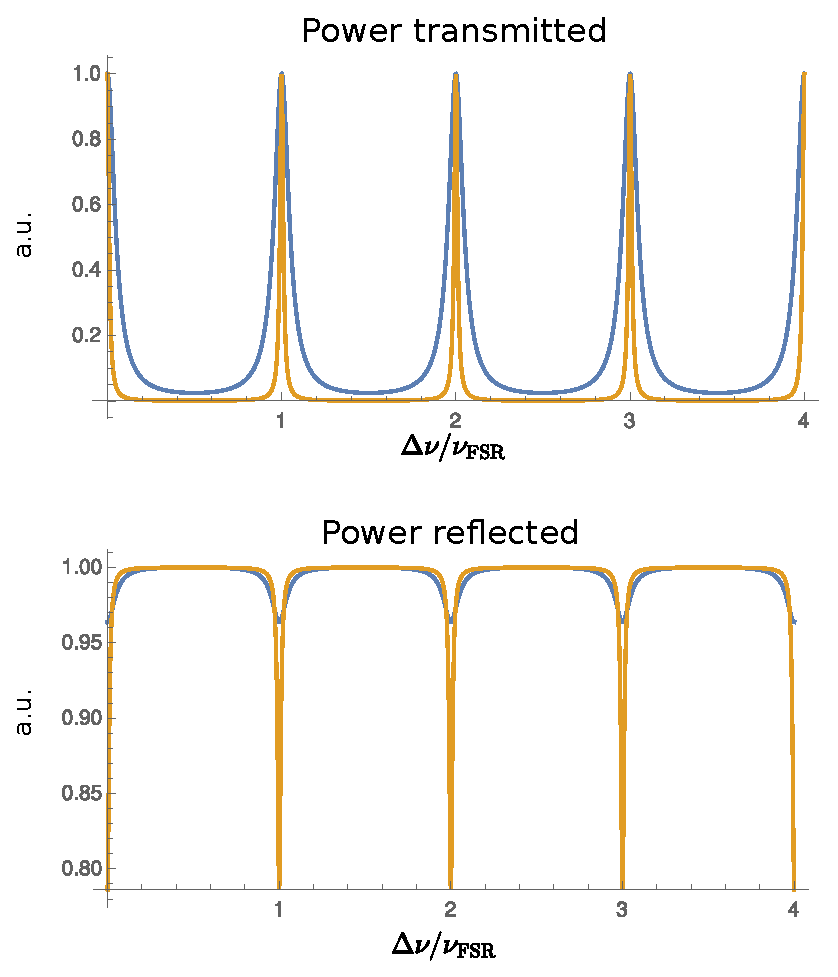
\includegraphics[width=0.9\linewidth]{images/reflected.eps}
	\caption{Transmission and reflection spectra of cavities with different Finesse (blue line for Finesse 10, orange for Finesse 50). The highest the Finesse the lowest the cavity bandwidth.}
	\label{fig:reflected}
\end{figure}

The field amplitude inside the Fabry-Perot cavity depends only on the mirror reflectivities. The field in a point inside the cavity must be equal to the sum of the same field after a round trip and the field that just entered the cavity through the first mirror, following Fig \ref{fig:ecav} we can write:
\begin{align}
	E_{\mathrm{cav}} &= \sqrt{1-R_1} E_{\mathrm{in}} +\sqrt{R_1R_2R_3R_4}e^{i\delta}E_{\mathrm{cav}} \\
	E_{\mathrm{cav}} &= \frac{\sqrt{1-R_1}}{1-\sqrt{R_1R_2R_3R_4}e^{i\delta}} E_{\mathrm{in}}
\end{align}
where $\delta=2\pi\Delta\nu/\nu_{\mathrm{FSR}}$ and $\Delta\nu=\nu-\nu_0$ is the ``detuning'' of the input frequency from the fundamental mode frequency.
From this we can derive the field transmitted through every mirror and the field reflected by the input coupler:
\begin{align}
E_{\mathrm{tr2}} &=  \sqrt{1-R_2}E_{\mathrm{cav}}\\
E_{\mathrm{tr3}} &=  \sqrt{(1-R_3)R_2}E_{\mathrm{cav}}\\
E_{\mathrm{tr4}} &=  \sqrt{(1-R_4)R_3R_2}E_{\mathrm{cav}}\\
E_{\mathrm{ref}} &=	 -\sqrt{R_1}E_{\mathrm{in}}+	\sqrt{(1-R_1)R_4R_3R_2}E_{\mathrm{cav}} \label{eq:ref}
\end{align}
The optical power inside the cavity will be given by $P_{\mathrm{cav}}\propto|E_{\mathrm{cav}}E_{\mathrm{cav}}^*|$ and the enhancement factor $P_{\mathrm{cav}}/P_{\mathrm{in}}$ can be calculated as:
\begin{align}
\frac {P_{\mathrm{cav}}}{P_{\mathrm{in}}} = \frac{1-R_1}{1+R-2\sqrt{R}\cos\delta}
\label{eq:power}
\end{align}
where $R=R_1R_2R_3R_4$.
Maximum power is reached for $\Delta\nu = n\nu_{\mathrm{FSR}}$, that is the resonance condition.

Another important property of a Fabry-Perot resonator is its Finesse, defined as the ratio between the free spectral range and the cavity linewidth. The cavity linewidth $\delta\nu$ can be found imposing $P_\mathrm{cav}(\delta\nu/2) = 1/2 P_\mathrm{cav}(0)$, a detuning of half linewidth reduce the power in the cavity by a factor of 2. This gives:
\begin{align}
\delta\nu = \nu_\mathrm{FSR} \frac{1-\sqrt{R}}{\pi R^{\frac{1}{4}}}
\end{align}
And so the Finesse is:
\begin{align}
	F = \frac{\nu_\mathrm{FSR}}{\delta\nu} = \frac{\pi R^{\frac{1}{4}}}{1-\sqrt{R}}
	\label{eq:finesse}
\end{align}
Transmission and reflection spectra of cavities with different Finesse are shown in Fig \ref{fig:reflected}.
The Finesse is related to the power gain of the cavity by
\begin{align}
	Gain = \frac{F}{a}
\end{align}
where $a$ is a numerical factor that tends to $\pi/2$ when the cavity losses are determined mainly by the input coupler transmission. Since $\pi/2$ is the minimum value assumed by $a$, this is the kind of cavity with maximum gain for a given Finesse, and the one used in BriXS. 

\subsection{Spectral coupling between cavity and oscillator}

To obtain maximum coupling between the cavity and the oscillator it is not enough to obtain spatial mode-matching (as described earlier by the overlap integral of Eq. \ref{eq:eta}), spectral matching between the two frequency combs must also be optimized.

\subsubsection{Effect of the $f_\mathrm{CEO}$}
The Carrier-Envelope-Offset (CEO) of the mode-locked laser (shown in Fig. \ref{fig:comb}) is a cause of mismatch between the spectral comb of the laser and that of the cavity.

The output field of a mode-locked laser can be described by the sum of the pulses:
\begin{align}
E(t) = \sum_{n} A(t-nt_r) e^{-i\omega_0 (t - nt_r)} e^{i \delta\Phi n}
\end{align}
where $A(t)$ is the pulse envelope, $\omega_0/2\pi$ is the carrier frequency, $t_r$ is the time between two successive pulses and $\delta\Phi$ is the CEO.
In the frequency domain it can be written (via Fourier transform):
\begin{align}
\tilde{E}(\omega) = \sum_n \tilde{B}(\omega) e^{i\omega n t_r} e^{i \delta\Phi n}
\end{align}
with $\tilde{B}(\omega)$ being the transform of $A(t) e^{-i\omega_0 t}$.
Because of the summation over $n$, the only frequencies $\omega_m$ that contribute are those that satisfy
\begin{align}
	\omega_m t_r + \delta \Phi = 2\pi m \\
	\omega_m = \frac{2\pi m}{t_r} -\frac{\delta \Phi}{t_r}
\end{align} 
Rewriting the last equation we get
\begin{align}
f_m = m f_\mathrm{rep} + f_\mathrm{CEO} && f_\mathrm{CEO} = -\frac{\delta \Phi}{2\pi t_r}
\end{align}
The cavity instead resonates at frequencies of the form:
\begin{align}
f_{cm} = m f_\mathrm{FSR}
\end{align}
with $f_\mathrm{FSR} = c/L$.
When the resonator and the oscillator are stabilized against each other we have that for a certain mode $m_0$ holds
\begin{align}
	m_0 f_\mathrm{rep} + f_\mathrm{CEO} = m_0 f_\mathrm{FSR}
\end{align}
In our cavity $m_0$ is about $L/\lambda_0=3\times10^6$. The relation doesn't hold for the other modes $m = m_0 +\delta m$, in fact the frequency mismatch between $f_m$ and $f_{cm}$ is given by 
\begin{align}
\Delta \nu &=  ((m_0+\delta m) f_\mathrm{rep} + f_\mathrm{CEO})-(m_0+\delta m)(f_\mathrm{rep} + f_\mathrm{CEO}/m_0)\\
\Delta \nu &= -f_\mathrm{CEO}\frac{\delta m}{m_0} = -f_\mathrm{CEO}\delta m\frac{\lambda_0}{L}
\end{align}
By writing the shift $\delta m $ in terms of a shift in wavelength
\begin{align}
	\delta m = \frac{\delta \nu}{f_\mathrm{rep}} = -\frac{c}{f_\mathrm{rep}\lambda_0^2}\delta\lambda
\end{align}
we finally get
\begin{align}
	\Delta \nu(\delta\lambda) = \frac{c f_\mathrm{CEO}}{f_\mathrm{rep}\lambda_0 L}\delta\lambda
\end{align}
$\Delta \nu$ is the difference between the laser mode frequency at $\lambda_0+\delta\lambda$ and the nearest cavity mode frequency.

An external mode will be coupled in the cavity only if $\Delta\nu(\delta\lambda)$ is within a cavity linewidth $\delta\nu_c$ from a cavity mode. The amount of modes coupled into the cavity depends on $f_\mathrm{CEO}$, i.e. the spectral coupling efficiency depends on $f_\mathrm{CEO}$. That means that if an incoming laser pulse has a spectrum of width $\Delta \lambda$:
\begin{align}
	S_\mathrm{in}(\delta\lambda) \propto \exp[-2 \frac{\delta\lambda^2}{\Delta\lambda^2}]
\end{align}
The pulse inside the cavity, and the pulse transmitted by the cavity, will have a spectrum:
\begin{align}
	S_\mathrm{out}(\delta\lambda) \propto S_\mathrm{in}(\delta\lambda)  \exp[-2\frac{\Delta\nu(\delta\lambda)^2}{\delta\nu_c^2}] 
\end{align}
The spectral coupling efficiency $\eta_\mathrm{sp}$ will then be given by the ratio of the two integrated spectra:
\begin{align}
	\eta_\mathrm{sp} = \frac{\int \exp[-2 \frac{\delta\lambda^2}{\Delta\lambda^2}]\exp[-2\frac{\Delta\nu(\delta\lambda)^2}{\delta\nu_c^2}]\,\mathrm{d}\delta\lambda}{\int \exp[-2 \frac{\delta\lambda^2}{\Delta\lambda^2}]\,\mathrm{d}\delta\lambda}
\end{align}

A plot of $\eta_\mathrm{sp}(f_\mathrm{CEO})$ is given in Fig \ref{fig:spectraleta} , we can see that to achieve bigger efficiency we can limit the spectrum entering the cavity, a feedback system to control the $f_\mathrm{CEO}$ (that depends on the temperature of the active medium) is also needed.
\begin{figure}
	\centering
	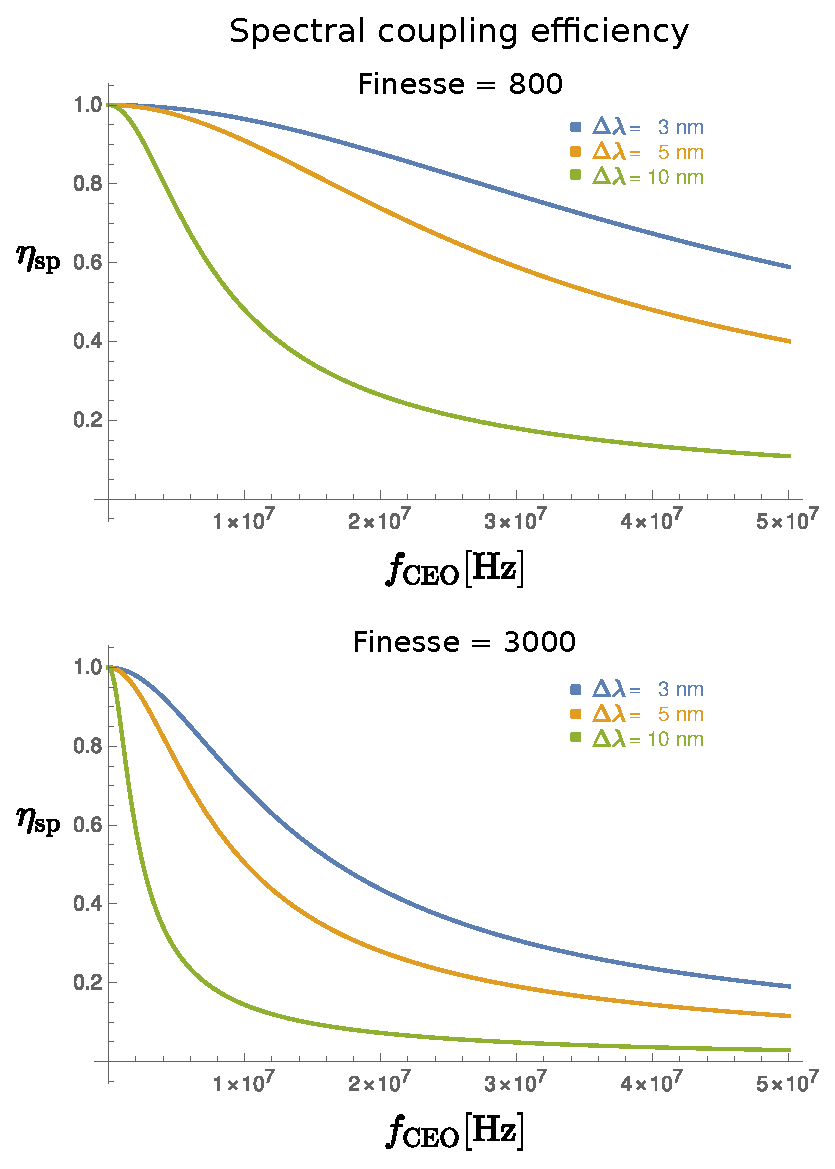
\includegraphics[width=0.9\linewidth]{images/spectraleta.eps}
	\caption{Spectral coupling efficiency as a function of the Carrier-Envelope-Offset frequency $f_\mathrm{CEO}$. The two plots refer to cavities with different Finesse: 800 for the top one and 3000 for the bottom one. The greater the Finesse, the greater the effect on the efficiency.}
	\label{fig:spectraleta}
\end{figure}

\subsubsection{Effect of the mirror dispersion}
When a laser beam reflects on a mirror it experiences a small phase shift $\phi(\lambda)$ caused by the fact that the penetration length is non-zero. This phase shift is different for each wavelength and it changes the effective length of the cavity according to
\begin{align}
	L_\mathrm{eff}(\lambda) = L + \frac{\lambda \phi(\lambda)}{2\pi}
\end{align}	
where $L$ is the length of the cavity while $L_\mathrm{eff}$ the effective length.
We can write the frequencies of the modes $\nu_m$ in a cavity $L_\mathrm{eff}(\lambda)$ long, each mode will see a different cavity length:
\begin{align}
	\nu_{m} = \frac{c}{L} \left( m_0 + \delta m - \frac{\phi(\lambda_{\delta m})}{2\pi} \right)
\end{align}
where as before we have $m = m_0 +\delta m$. If we expand $\phi(\lambda)$ to second order we get:
\begin{align}
	\nu_{m} = \frac{c}{L} \left( m_0 + \delta m -\frac{\phi_0}{2\pi} -\frac{1}{2\pi} \frac{\partial\phi}{\partial\lambda} \delta\lambda - \frac{1}{4\pi} \frac{\partial^2\phi}{\partial\lambda^2} \delta\lambda^2  \right)
\end{align}

Since $\delta\lambda \propto \delta m$, the first order term simply changes the spacing between the cavity resonant frequency by a fixed amount, and can be corrected by changing $L$. The second order term changes instead the spacing between the modes by a different amount for each $m$, introducing again a mismatch between the cavity resonant frequencies and the laser modes. The second order term can be estimated using dielectric mirror theory \parencite{Garmire2003} to
\begin{align}
	\frac{\partial^2\phi}{\partial\lambda^2} = -2.084\times 10^{-5}\,\mathrm{nm}^{-2}
\end{align}
for TiO$_2$-SiO$_2$ mirrors. A plot of the effect of the mirror dispersion on the coupling efficiency is shown in Fig \ref{fig:dispersion}, we can see that for our current Finesse a spectrum of width $\Delta\lambda = 3\,$nm is sufficient while for the final cavity the spectrum must be narrower. The mirror dispersion effect on the coupling efficiency cannot be compensated (as opposed to that given by the $f_\mathrm{CEO}$) and so constitutes a limiting factor on the spectrum that can be coupled in the final Fabry-Perot cavity.
\begin{figure}
	\centering
	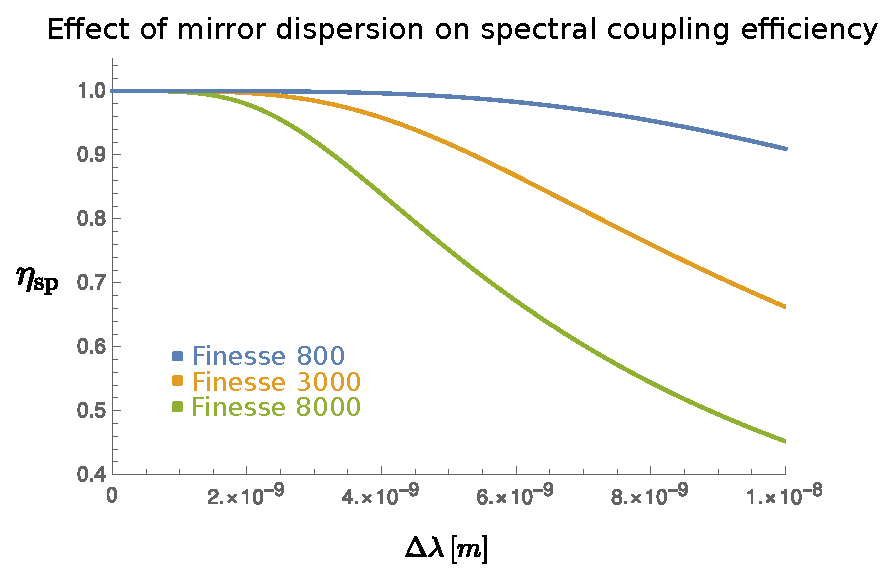
\includegraphics[width=0.9\linewidth]{images/dispersion.eps}
	\caption{Effect of the mirror dispersion on the spectral coupling efficiency. The effect is greater for higher Finesse. The only way to mitigate the effect is to reduce the input radiation spectral width.}
	\label{fig:dispersion}
\end{figure}

\subsection{Thermal effects and the compensation method}
\begin{figure}
	\centering
	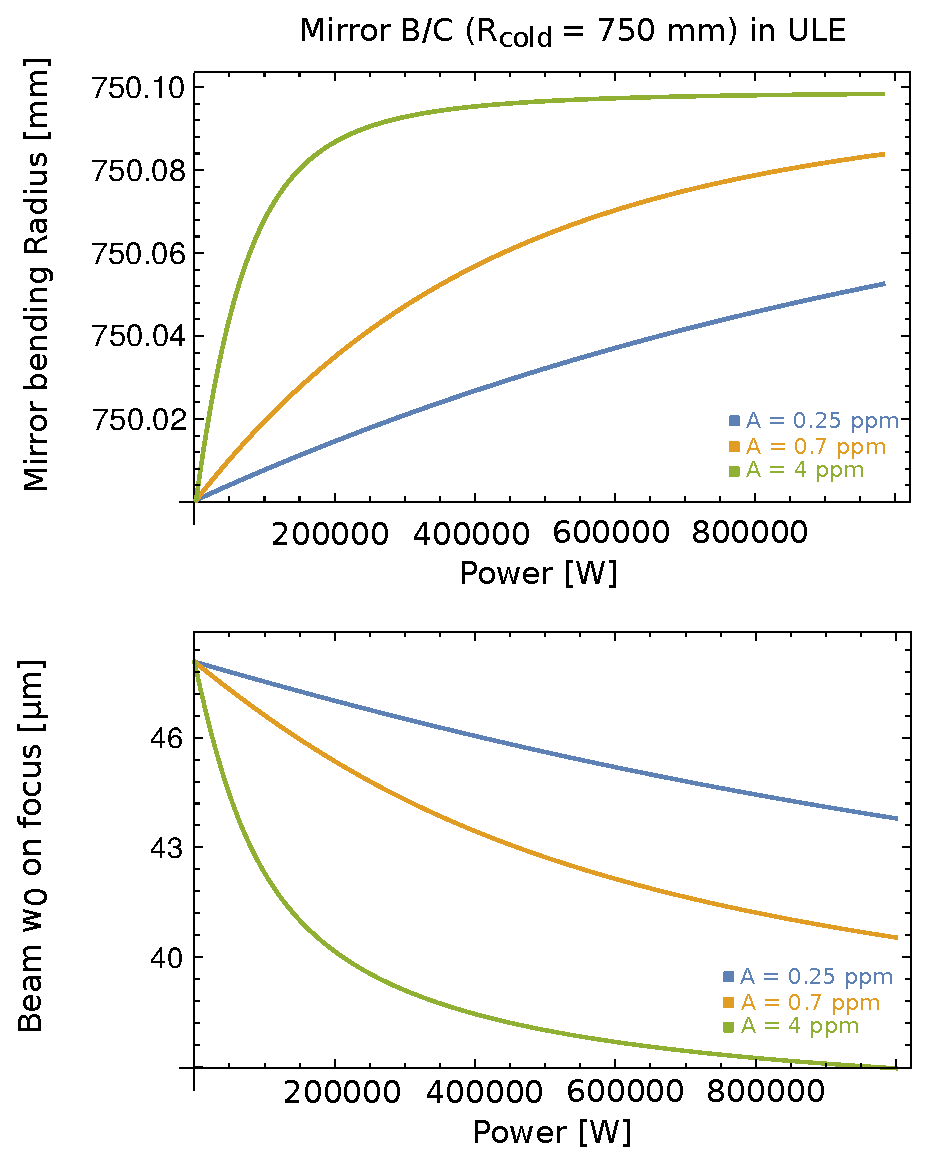
\includegraphics[width=0.9\linewidth]{images/mirrordef.eps}
	\caption{Top: radius of curvature of mirrors B and C versus power. The substrate material of choice for BriXS is ULE (Ultra Low Expansion) for its reduced thermal deformation. Bottom: waist size versus power, to compensate for the waist size change the distance between mirrors B and C has to be corrected. Different colors refer to different mirror absorption.}
	\label{fig:mirrordef}
\end{figure}
\begin{figure}
	\centering
	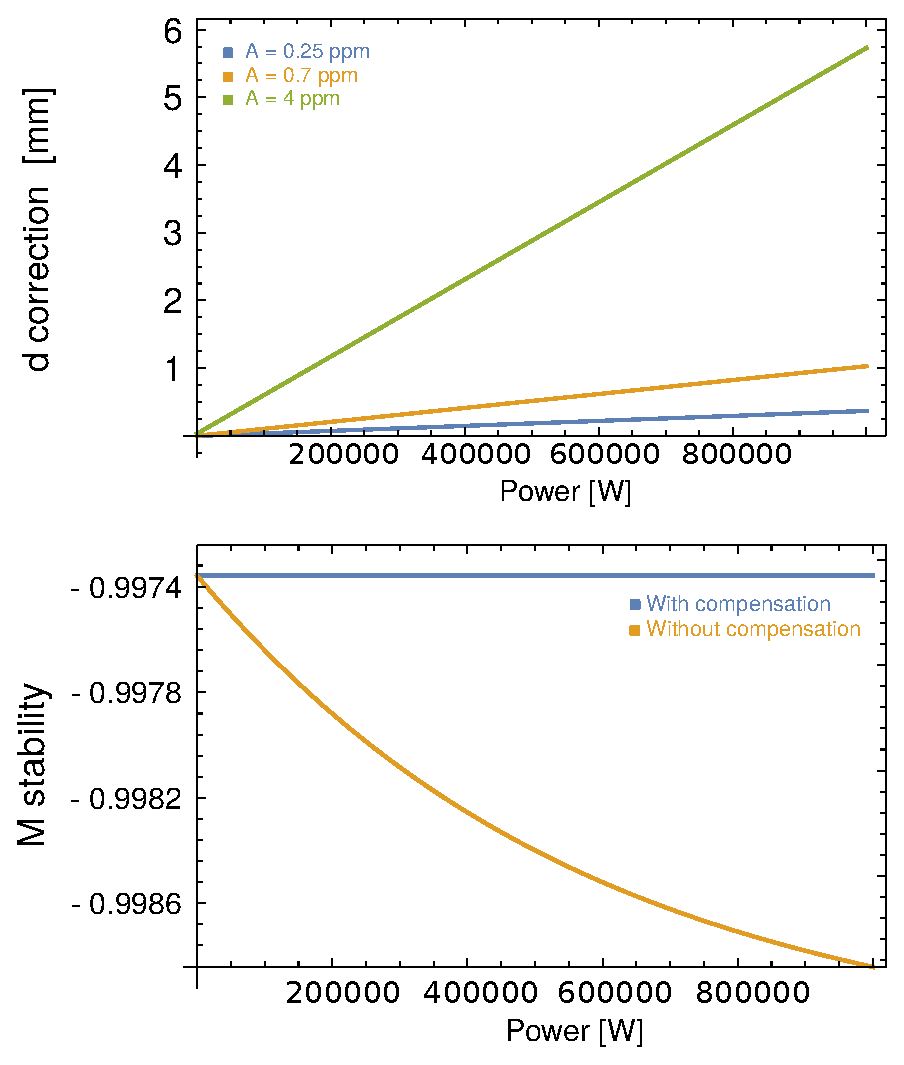
\includegraphics[width=0.9\linewidth]{images/compensation.eps}
	\caption{Top: correction length for the curved mirror distance B-C as a function of cavity internal power. Bottom: stability parameter $m_V$ as a function of cavity internal power, without compensation the stability parameter goes towards the stability edge $m=-1$, by implementing the correction from the top plot the stability parameter is kept constant.}
	\label{fig:compensation}
\end{figure}
\begin{figure}
	\centering
	\includegraphics[width=0.9\linewidth]{images/spotdim.pdf}
	\caption{Top: Spot size on the input mirror A, as the cavity becomes near-confocal the spot size increases, diminishing the thermal deformation. Bottom: Waist size in the cavity focus, in the near-confocal configuration the size vanishes. The difference between the vertical and horizontal size is a consequence of the astigmatism of the curved mirrors, which have a different effective radius in the two directions.}
	\label{fig:spotdim}
\end{figure}

In a high-gain Fabry-Perot cavity the internal power can cause the mirrors to change shape because of the thermal deformation of the mirror surface. In particular a mirror heated by a gaussian beam gains an additional curvature given by \parencite{Winkler1991}:
\begin{align}
\frac{1}{R_t} = -\gamma \frac{a}{k} \frac{P}{2\pi w^2}
\end{align}
where $k$ is the thermal conductivity, $a$ the expansion coefficient, $\gamma$ the mirror absorption and $P$ the optical power.
The total radius can then be found as:
\begin{align}
	\frac{1}{R_\mathrm{warm}} = \frac{1}{R_\mathrm{cold}} +  \frac{1}{R_t}
\end{align}
The waist size and the spot size at the mirrors surface both depend on the radius of curvature, this means that they also depend on the internal power of the cavity. In \ref{fig:mirrordef} we can see the relation between the waist size and the internal optical power: as the radius of curvature gets bigger so does the cavity waist. The size depends also on the curved mirror separation (for our cavity the relation is shown in Fig \ref{fig:spotdim}): it is then possible to calculate a mirror separation B-C that keeps the cavity focus at the same size for every power. Since the cavity must maintain its length to couple with the laser, we simultaneously have to change the position of mirror D. This ``compensation method'' can be realized by mounting the mirrors on piezoelectric driven sleds, an essential requirement is that the cavity remains stabilized during the movement.

\subsubsection{Degenerate mode coupling}

It is known that in a high-Finesse optical resonator non-ideal effects like mirror roughness and non-infinite mirror size can cause unwanted losses through
a process known as resonant mode coupling \parencite{Klaassen2005,Kleckner2010,Benedikter2015}. When two cavity modes have the same resonant frequency, energy transfer can occur between them because of cavity non-idealities, such as mirror roughness or finite size. This can lead to increased losses as the coupling between the cavity fundamental mode and the external oscillator mode is reduced. Frequency degeneracy can occur for particular cavity geometries (which translates to particular $m_V$ and $m_H$ parameters), since thermal expansion can change the stability parameters mode coupling can be a problem for BriXS cavities.
\begin{figure}
	\centering
	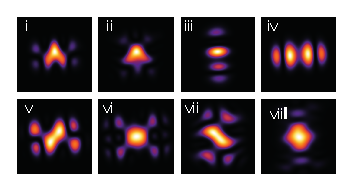
\includegraphics[width=0.9\linewidth]{images/modemixing.eps}
	\caption{Possible cavity fundamental eigenmodes when resonant mode coupling occurs, observed by \parencite{Benedikter2015} by varying the cavity length. The fundamental mode consists of a superposition of the $HG_{00}$ with a higher order mode, such as the $HG_{14}$ in figure $\boldsymbol{i}$.  }
	\label{fig:modemixing}
\end{figure}

To account for mirror surface imperfections and finite size, we introduce the ``mode-mixing operator'' \parencite{Kleckner2010}:
\begin{align}
\mathrm{M}=\exp(ikL)\mathrm{A}\times{B}
\end{align}
where A and B represent the effect of mirrors on the mode (and may be more than two,
our cavity has four mirrors).
Cavity modes $\ket{\psi_\mathrm{i}}$ (we use Dirac notation) satisfy:
\begin{equation}
\gamma_\mathrm{i}\ket{\psi_\mathrm{i}} = \mathrm{M}\ket{\psi_\mathrm{i}}
\end{equation}
where $\gamma_\mathrm{i}$ must be real for the mode to resonate and $D=1-|\gamma_\mathrm{i}|^2$ represents the power loss after a round trip. The ``ground state'' of the cavity is the mode with minimum power loss.
We can express the mirror operators A and B and the mode-mixing operator M in the Hermite-Gauss basis $\{\ket{\phi_{nm}}\}$:
\begin{equation}
\label{A}
\mathrm{A}_{nm,st} = \frac{1}{T}\int dt\iint_S dxdy\ \phi_{nm}\phi_{st}^*e^{-2ik\Delta_a(x,y)}
\end{equation}
where $\Delta_a(x,y)$ is the deviation of the mirror from a plane given by the mirror roughness (the factor 2 is needed to account both for the incident and the reflected beam) and $\phi_i$ are the Hermite-Gauss modes (see \ref{eq:HG}). The spatial integral is taken over the surface of the mirror and the temporal integral averages the value over multiple round trips. This is very important because then $\mathrm{A_{nm,st}}$ is non-zero only if the two modes share the same frequency $\nu$. In the case of perfect mirrors A is the identity matrix and the cavity eigenmodes correspond to the Hermite-Gauss set, with $HG_{00}$ as fundamental mode. If $\Delta_{a,b}(x,y) \ne 0$ A and M are not diagonal and energy transfer occurs between the Hermite-Gauss modes. The new eigenmodes of the cavity are given by diagonalizing M and will in general be superpositions of the HG modes (see Fig \ref{fig:modemixing}). When this happens the coupling between the external ($HG_{00}$) mode and the cavity eigenmode is reduced as their overlap integral becomes smaller.  We note that the overlap integral \ref{A} of a $HG_{nm}$ mode with the $HG_{00}$ becomes smaller the greater $n+m$ is, so we expect higher order modes to contribute less to mode coupling.

In a cavity affected by mode coupling the internal power undergoes periodical fluctuations: firstly thermal deformations introduce losses through mode coupling, these losses reduce the internal power, the temperature of the mirror decreases restoring their shape, now the power can increase again and the process restarts.

The ``compensation method'' used to change the cavity waist size can also be employed to avoid cavity modes to become degenerate by controlling the $m$ parameters of the cavity.
	\chapter[Stabilization through feedback]{The PDH technique and stabilization through feedback}
The cavity being stabilized in frequency is what makes the ICS source of MariX possible; given its importance, in this brief chapter I will explain how the PDH technique works and how it has been implemented in our cavity.

\section{The PDH technique}
The Pound-Drever-Hall technique \parencite{Black2001} provides a method for locking the cavity frequency to the external laser reference.

When a cavity is perfectly resonant with an external laser mode the reflected power experiences a minimum while the transmitted power a maximum (see Fig \ref{fig:reflected}), one can then see that both these intensity signals cannot be used to provide a correction should the cavity resonant frequency change, as they both are symmetric signals.
We note that the reflected field is composed of two contributions: the reflected beam from the first mirror and the transmitted beam from the cavity through the first mirror, the first field carries a phase factor $-1$ while the second $e^{-i(\omega-\omega_0)/\nu_\mathrm{FSR}}$. The resulting sum will then have a phase dependent on $\omega-\omega_0$. Recalling eq. \ref{eq:ref} we can write the normalized reflected field:
\begin{align}
	F(\omega) = \frac{E_\mathrm{ref}}{E_\mathrm{in}} = \frac{\sqrt{R} \left(e^{-i(\omega-\omega_0)/\nu_\mathrm{FSR}}-1\right)}{1-R e^{-i(\omega-\omega_0)/\nu_\mathrm{FSR}}}
\end{align}
where $R$ is the total mirror reflectivity, $\omega_0$ the resonance frequency and $\nu_{\mathrm{FSR}}$ the free spectral range. As can be seen in Fig \ref{fig:fomega}, the phase of the reflected phase is asymmetric, i.e. it can be used as an error signal to stabilize the cavity length.
\begin{figure}
	\centering
	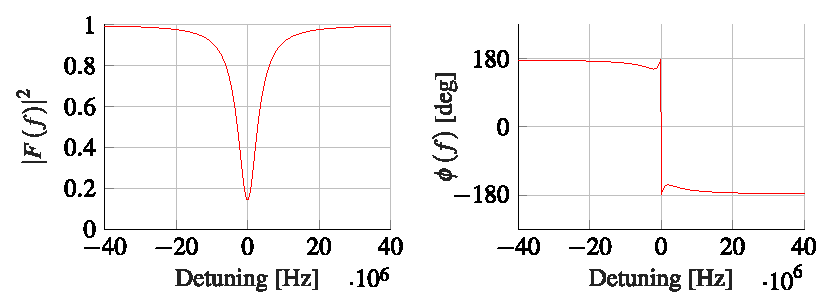
\includegraphics[width=0.9\linewidth]{images/fomega.eps}
	\caption{Module and phase of the field reflected from a Fabry-Perot cavity, while the module is symmetric with the detuning of the incident field, the phase is asymmetric and can thus be used as an error signal.}
	\label{fig:fomega}
\end{figure}

We cannot directly measure the phase of the field with a photodetector, but this is where the PDH technique comes into play: consider a phase modulator, such as an electro-optic modulator, constructed with a nonlinear crystal able to rapidly modulate its refractive index in relation to an applied voltage. The relevant relation is:
\begin{align}
n(E) = n_e - \frac{1}{2}n_e^3 r_{33}E
\end{align}
where $n_e$ is the extraordinary index of the birefringent crystal, $r_{33}$ the relevant component of the electro-optical tensor and $E$ the applied field. If we apply a sinusoidal voltage $V(t) = Ed = V_0 \sin\Omega t$ to the crystal, the radiation passing through the crystal will be described by:
\begin{align}
	E(t) &=  E_0 \exp[-i\omega t + i\,2\pi\, n(t)\, z/\lambda] =\\
		&= E_0 \exp\left[-i\omega t +i\omega \frac{z}{c}(n_e - \frac{1}{2}n_e^3 r_{33}\frac{V_0}{d}\sin\Omega t) \right]
\end{align}

By defining $\beta = \frac{1}{2}\frac{\omega z}{c}n_e^3\frac{V_0}{d}r_{33}$ and redefining $\tilde E_0 = E_0 \exp(i\omega n_e z/c)$ we get
\begin{align}
E(t) = \tilde E_0 \exp(i\omega t)\exp(i\beta \sin\Omega t)
\end{align}

We can expand this result to first order using the Bessel functions $J_k$, obtaining
\begin{align}
	E(t) &\approx \tilde E_0 [J_0(\beta) + 2 i J_1(\beta) \sin\Omega t]\exp(i\omega t )\\
	&= \tilde E_0 [J_0(\beta)e^{i\omega t} + J_1(\beta)e^{i(\omega+\Omega) t} -J_1(\beta)e^{i(\omega-\Omega) t}]
\end{align}

That is, if a single frequency $\omega$ enters the EOM, three different frequencies compose the radiation coming out of the EOM: the carrier $\omega$ and two sidebands $\omega\pm\Omega$. The expansion holds for small modulation ($\beta < 1$).
If this field enters the cavity, the reflected field will be
\begin{align}
	E(t) = \tilde E_0 [F(\omega)J_0(\beta)e^{i\omega t} + F(\omega+\Omega)J_1(\beta)e^{i(\omega+\Omega) t} -F(\omega-\Omega)J_1(\beta)e^{i(\omega-\Omega) t}]
\end{align}

To find an expression for the optical power, which is what the photodiode measures, we consider that $\Omega \gg \delta\omega$ (sidebands distance from the carrier much larger than the cavity linewidth\footnote{This means that while the carrier frequency is coupled with the cavity, the sidebands are completely reflected.}), that $J_\alpha(\beta)\approx \frac{1}{\Gamma(\alpha+1)}\left(\frac{\beta}{2}\right)^2$ and that $P_c \gg P_s$ (power of the carrier much larger than that of the sidebands), after some algebra we get
\begin{align}
	P_\mathrm{ref} \approx P_c |F(\omega)|^2 -2 P_c\beta\Im{F(\omega)}\sin\Omega t + (2\Omega \,\mathrm{terms})
\end{align}

We can now see that it is possible to measure $\Im{F(\omega)}$, all is needed is to remove the $\sin\Omega t$ term with a demodulation (using for example a mixer) and then filter out the $2\Omega$ terms with a low-pass filter.

The full PDH error signal, after demodulating and filtering, is
\begin{align}
	\epsilon_\mathrm{PDH} = -\frac{1}{2}P_c\beta \Im{F(\omega)F^*(\omega+\Omega)-F^*(\omega)F(\omega-\Omega)}
\end{align}
represented in Fig \ref{fig:errsignal}.
Near resonance the error signal has a ``linear zone'': in fact in this case we can write
\begin{align}
	\omega = 2\pi N \nu_\mathrm{FSR} + \delta\omega
\end{align}
where $\delta\omega$ is the detuning from resonance, and from this we get
\begin{align}
	F(\delta\omega) \approx \frac{i}{\pi}\frac{\delta\omega}{\delta\nu}
\end{align}
where $\delta\nu$ is the cavity linewidth. The error signal near resonance then becomes
\begin{align}
	\epsilon_\mathrm{PDH} \approx -\frac{2}{\pi}P_c \beta \frac{\delta\omega}{\delta\nu}
\end{align}
where it is clear its linear dependence from $\delta\omega$. This approximation holds for high finesse caivities and for $\delta\omega \ll \delta\nu$.

\begin{figure}
	\centering
	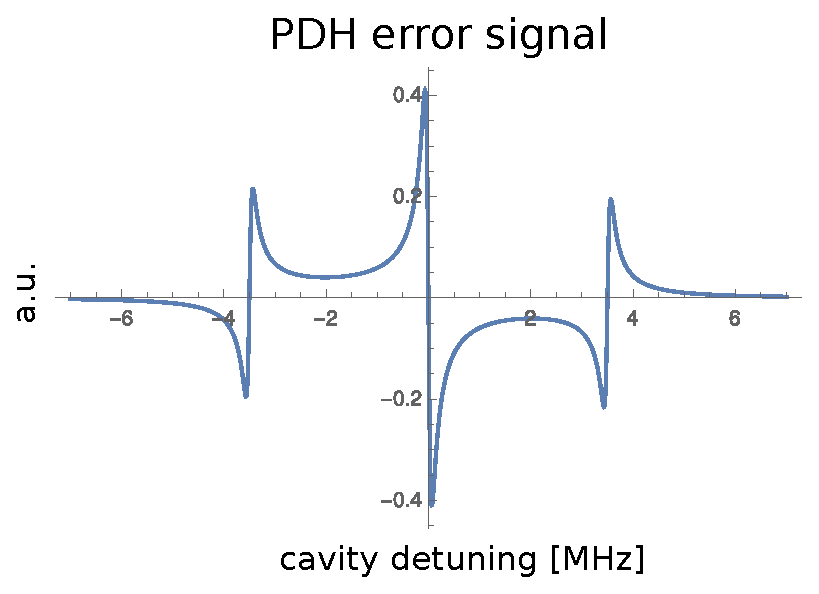
\includegraphics[width=0.8\linewidth]{images/errsignal.eps}
	\caption{The typical PDH error signal. The carrier-sidebands distance is 3.5\,MHz as in our experimental setup. The linear zone can be seen in the center.}
	\label{fig:errsignal}
\end{figure}

\section{Feedback system}

We have seen that the PDH stabilization technique is based on a feedback loop, we now wish to study the stability properties of this loop.

The system can be divided in 5 parts:
\begin{enumerate}
	\item A reference: in our case the mode-locked laser
	\item A source: the Fabry-Perot cavity
	\item A discriminator: the electronic system that generates the error signal, composed by a EOM, a detector, a phase shifter, a mixer and a low-pass filter
	\item A servo: the PID that uses the error signal to drive the piezo
	\item An actuator: the piezo that moves the mirror inside the cavity.
\end{enumerate}
\begin{figure}
	\centering
	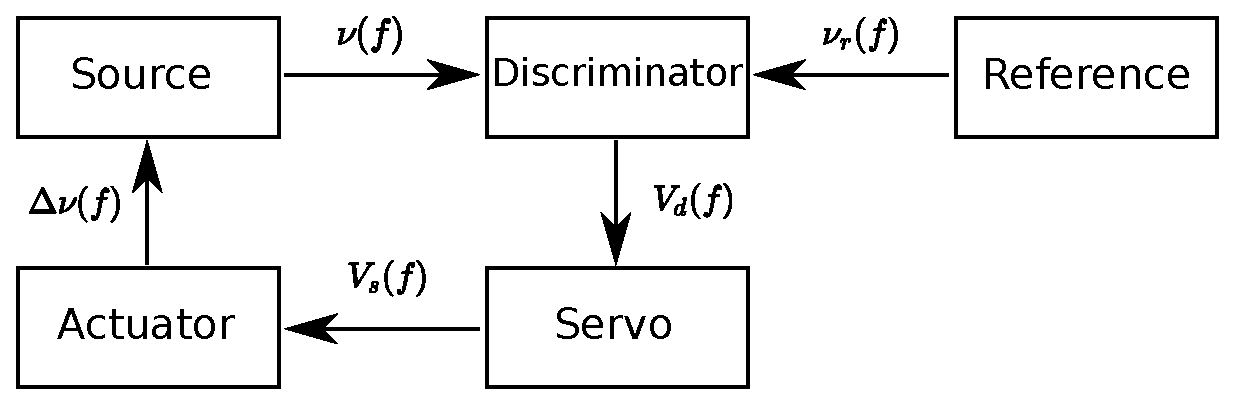
\includegraphics[width=0.9\linewidth]{images/loop.eps}
	\caption{The stabilization system feedback loop.}
	\label{fig:loop}
\end{figure}

The feedback loop is showed in Fig \ref{fig:loop}.

\subsubsection{Discriminator}
Let's consider the frequency signal generated by the reference $\tilde \nu_r(t)$ and that of the source $\tilde \nu(t)$, the purpose of the feedback loop it to minimize $\Delta\tilde\nu = |\tilde\nu_r(t)-\tilde\nu(t)|$. In the Fourier domain the signals are $\nu(f)$ and $\nu_r(f)$, these signals are combined by the discriminator, which outputs a voltage proportional to their difference, that is
\begin{align}
	V_D = D(f) (\nu(f)-\nu_r(f))
\end{align}
where $D(f)$ is the frequency response. From Fig \ref{fig:errsignal} we can see that the frequency response is essentially a constant, the slope of the linear zone $k_d$, multiplied by  the 6th-order Butterworth filter response. The typical Butterworth filter response is shown in Fig \ref{fig:servo}, while the $k_d$ constant can be measured from the error signal during a scan, if $2\Omega =7$\,MHz is the frequency distance between the sidebands, $\Delta t$ their temporal separation during a scan, $\delta V/\delta t$ the difference quotient of two points in the linear zone:
\begin{align}
	k_d = \frac{\delta t}{\delta V} \frac{2\Omega}{\Delta t}
\end{align}

\subsubsection{Servo}
The servo elaborates the error signal and outputs the right voltage to the piezo.
After passing through the servo, the voltage signal becomes
\begin{align}
	V_s = S(f) V_d = S(f)D(f)(\nu(f)-\nu_r(f))
\end{align}
\begin{sidewaysfigure}
	\centering
	\includegraphics[width=0.9\linewidth]{images/pidscheme.pdf}
	\caption{The servo PID circuit.}
	\label{fig:servoscheme}
\end{sidewaysfigure}

where $S(f)$ is the servo PID transfer function. The servo schematic is shown in Fig \ref{fig:servoscheme}: first the error signal goes through an Offset stage, where a DC component can be added to it, then it goes through both the Proportional and Integrator stages, the outputs of which are summed in a summer stage. The signal is then filtered with a single pole LP filter and sent to an amplifier (of fixed gain 3). We must include the piezo actuator response in the circuit: the piezo behaves essentially like a capacitor $C$ in the system, since the PID has output resistance $R$ it constitutes a LP filter with characteristic time $\tau = RC$. All the stages contribute to the frequency response via their transfer functions $G_i$:
\begin{align}
	S(f) = G_\mathrm{offset}(f)[G_\mathrm{int}(f)+G_\mathrm{prop}(f)]G_\mathrm{filter}(f)G_\mathrm{piezo}(f)
\end{align}
where the summer and amplifier stages are considered to have unitary gain (they are composed of Op-Amps in retroactive feedback configuration). The typical servo transfer function is shown in Fig \ref{fig:servo}.
\begin{figure}
	\centering
	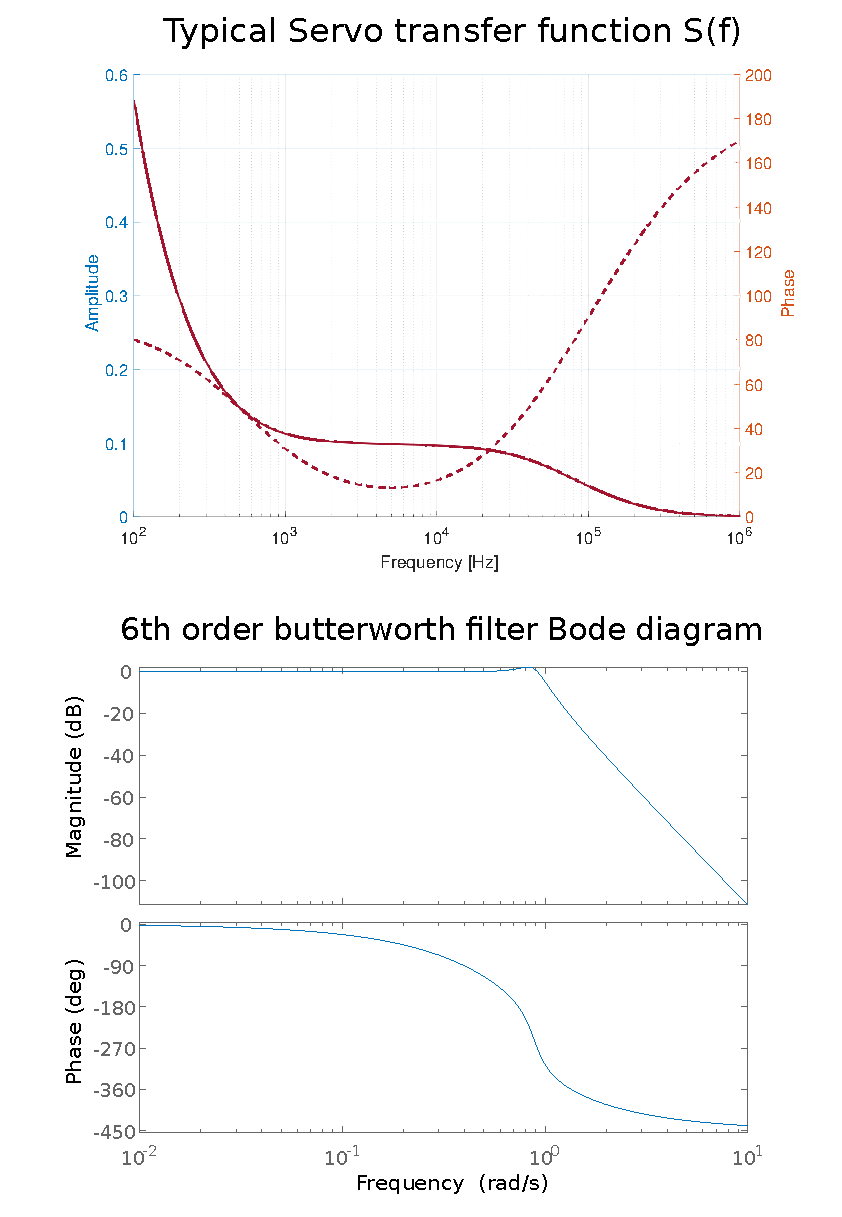
\includegraphics[width=0.8\linewidth]{images/servo.eps}
	\caption{Top: Servo transfer function S(f), the continuous line indicates the amplitude while the dotted one the phase.	Bottom: 6th order Butterworth filter transfer function.}
	\label{fig:servo}
\end{figure}

\subsubsection{Actuator}

The piezo actuator moves the first mirror of the cavity and in doing so converts the voltage signal received by the PID to a frequency signal $\Delta \nu$, that is the change in resonant frequency of the cavity:
\begin{align}
	\Delta \nu(f) = A(f)V_s = A(f)S(f)D(f)(\nu(f)-\nu_r(f))
\end{align}
where $A(f) = k_a \tilde A(f)$ is the piezo transfer function. The piezo, being a moving object, has a frequency response that depends on its mechanical properties and that of its mounting ($\tilde A(f)$), and by acting on the cavity provides a voltage-to-frequency conversion $k_a$. To characterize such a response we built a Michelson interferometer, using the fringes to measure the piezo movement in response to an applied sinusoidal voltage. By choosing the DC component of the sinusoidal voltage in order to place the piezo around the linear part of the fringes, a linear relation between intensity of the fringe and piezo movement can be obtained. Results are shown in Fig \ref{fig:actuator}, the piezo presents a resonance similar to that of an harmonic oscillator near 23000\,Hz. Another part of the transfer function is the voltage-to-frequency conversion ratio $k_a$, this can be measured by observing the transmitted beam. In fact the difference in cavity length between two resonances is $\lambda = 1030\,nm$ and by measuring the change in voltage on the piezo between two peaks the voltage/length relation is found, this can be then converted to a voltage/frequency conversion remembering that $\nu_\mathrm{FSR} = c/L$.
\begin{figure}
	\centering
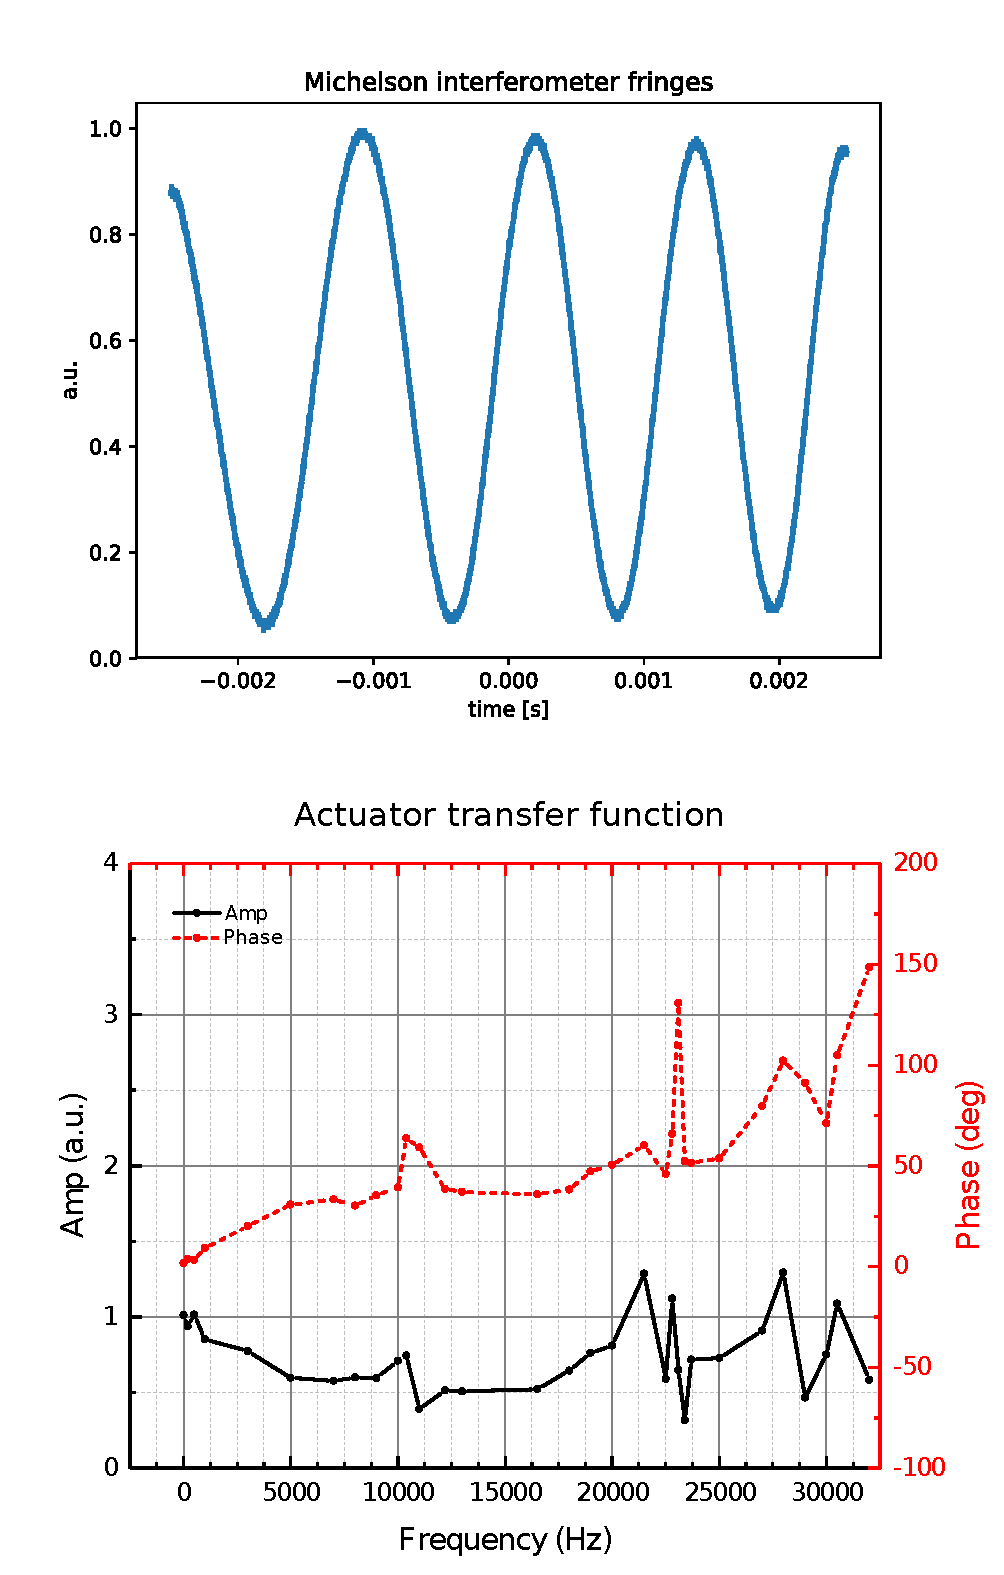
\includegraphics[width=0.8\linewidth]{images/actuator.eps}
\caption{Top: Michelson interference fringes observed by moving the piezo. Around 0.5\,V the movement/intensity relation is linear, so by sending a small sinusoidal voltage we can measure the piezo movements with a photodetector. Bottom: Actuator transfer function measured with the interferometer, for every point a sinusoidal voltage with the desired frequency has been sent to the piezo and the phase and amplitude of the resulting movement recorded.}
\label{fig:actuator}
\end{figure}

\subsubsection{Feedback loop}

The overall transfer function of the system is given by
\begin{align}
	G(f) = A(f)S(f)D(f)
\end{align}
and the actuator changes the resonant frequency of the FP cavity according to (we drop the $f$ dependence):
\begin{align}
	\nu = \nu_0 + ASD(\nu_r-\nu)
\end{align}
where $\nu_0$ is the original cavity frequency. To find the closed loop gain of the system we explicit $\nu$:
\begin{align}
	\nu = \frac{1}{1+G}\nu_0 + \frac{G}{1+G}\nu_r
\end{align}
From this equation we see that to lock the resonant frequency $\nu$ to the reference $\nu_r$ we need the absolute value of G to be as high as possible, in fact in this limit:
\begin{align}
	\frac{1}{1+G} \rightarrow 0 && \frac{G}{1+G} \rightarrow 1
\end{align}
meaning that $\nu=\nu_r$.

We can then calculate how the noises on the source and on the reference (the stochastic processes identified by $\nu(f)$ and $\nu_r(f)$ respectively) are suppressed by the feedback loop, resulting in low relative noise $\Delta\nu(f) = \nu_r(f) -\nu(f)$ between the two. To calculate the power spectral density noise of $\Delta\nu$ we take
\begin{align}
	|\Delta\nu(f)|^2 &= |\nu_r(f) - \nu(f)| ^ 2 =\\
			&= |\nu_r(f)|^2 + |\nu_(f)|^2 -2\Re{\nu(f)\nu_r(f)^*} = \\
			&= |\nu_r(f)|^2 + \left|\frac{1}{1+G(f)}\nu_0(f) + \frac{G(f)}{1+G(f)}\nu_r(f)\right|^2 +\\
			&- 2 \Re{\left(\frac{1}{1+G(f)}\nu_0(f)+\frac{G(f)}{1+G(f)}\nu_r(f)\right)\nu_r(f)^*}
\end{align}

We can assume that the two processes $\nu_r(f)$ and $\nu_0(f)$ are uncorrelated, since they refer to different systems, this means that mixed terms like $\nu_r(f)\nu(f)$ don't contribute, so we can write
\begin{align}
		|\Delta\nu(f)|^2 &= |\nu_r(f)|^2 + \frac{1}{\left|1+G(f)\right|^2}|\nu_0(f)|^2 + \frac{|G(f)|^2}{\left|1+G(f)\right|^2}|\nu_r(f)|^2 +\\ &-2\Re{\frac{G(f)}{1+G(f)}|\nu_r(f)|^2} = \\
		&=\frac{1}{\left|1+G(f)\right|^2}|\nu_0(f)|^2 + \frac{1}{\left|1+G(f)\right|^2}|\nu_r(f)|^2
\end{align}
Writing in terms of the power spectral densities $S_{\Delta\nu}(f)$, $S_{r}(f)$ and $S_{0}(f)$:
\begin{align}
S_{\Delta\nu}(f) = \frac{1}{\left|1+G(f)\right|^2} \left[S_{0}(f) + S_{r}(f)\right]
\end{align}
It is clear that by maximizing the loop gain, in particular by maximizing $\left|1+G(f)\right|^2$, the noise between source and reference is suppressed.

Feedback instabilities can arise when $G(f)=-1$: if this relation is satisfied for some $f$ then the system will oscillate at that frequency. This is the so-called Barkhausen stability criterion: when the phase of the loop gain $G$ is close to $\pi +2n\pi$ its absolute value must be $|G|\ne1$ to avoid auto-oscillations. Satisfying this criterion is the purpose of the LP single pole filter in the servo PID: by regulating the cutoff frequency we can make sure that $|G|<1 $ when $\angle G \approx \pi +2n\pi$.

The stabilization procedure will be explained in the next chapter, where also the  measurements of the Power Spectral Density noise of the stabilized cavities will be presented.

\begin{figure}
	\centering
	\includegraphics[width=0.7\linewidth]{images/foto/actuator.jpg}
	\caption{The mirror A mounting containing the piezo ring actuator.}
	\label{fig:fotoactu}
\end{figure}
\begin{figure}
	\centering
	\includegraphics[width=0.9\linewidth]{images/foto/discr.jpg}
	\caption{The discriminator stage. Left: the photodetector monitoring the blue cavity reflected beam. Right: phase shifters, mixers, and LP filters for both the cavities, the PDH signal is sent from the filters to the servo PID. }
	\label{fig:discr}
\end{figure}
\begin{figure}
	\centering
	\includegraphics[width=0.9\linewidth]{images/foto/pid.png}
	\caption{The servo stages used to drive the piezo in both cavities. }
	\label{fig:pid}
\end{figure}
	\chapter{Experimental Results}

In this chapter I will present the experimental setup and results obtained during this thesis realization. Most of the results concern the characterization of the two cavities, their stabilization and their noise profile. Another important conclusion is the possibility of moving the cavity waists, enabling the dual color mode of BriXS. 

\section{Experimental setup}
\begin{figure}
	\centering
	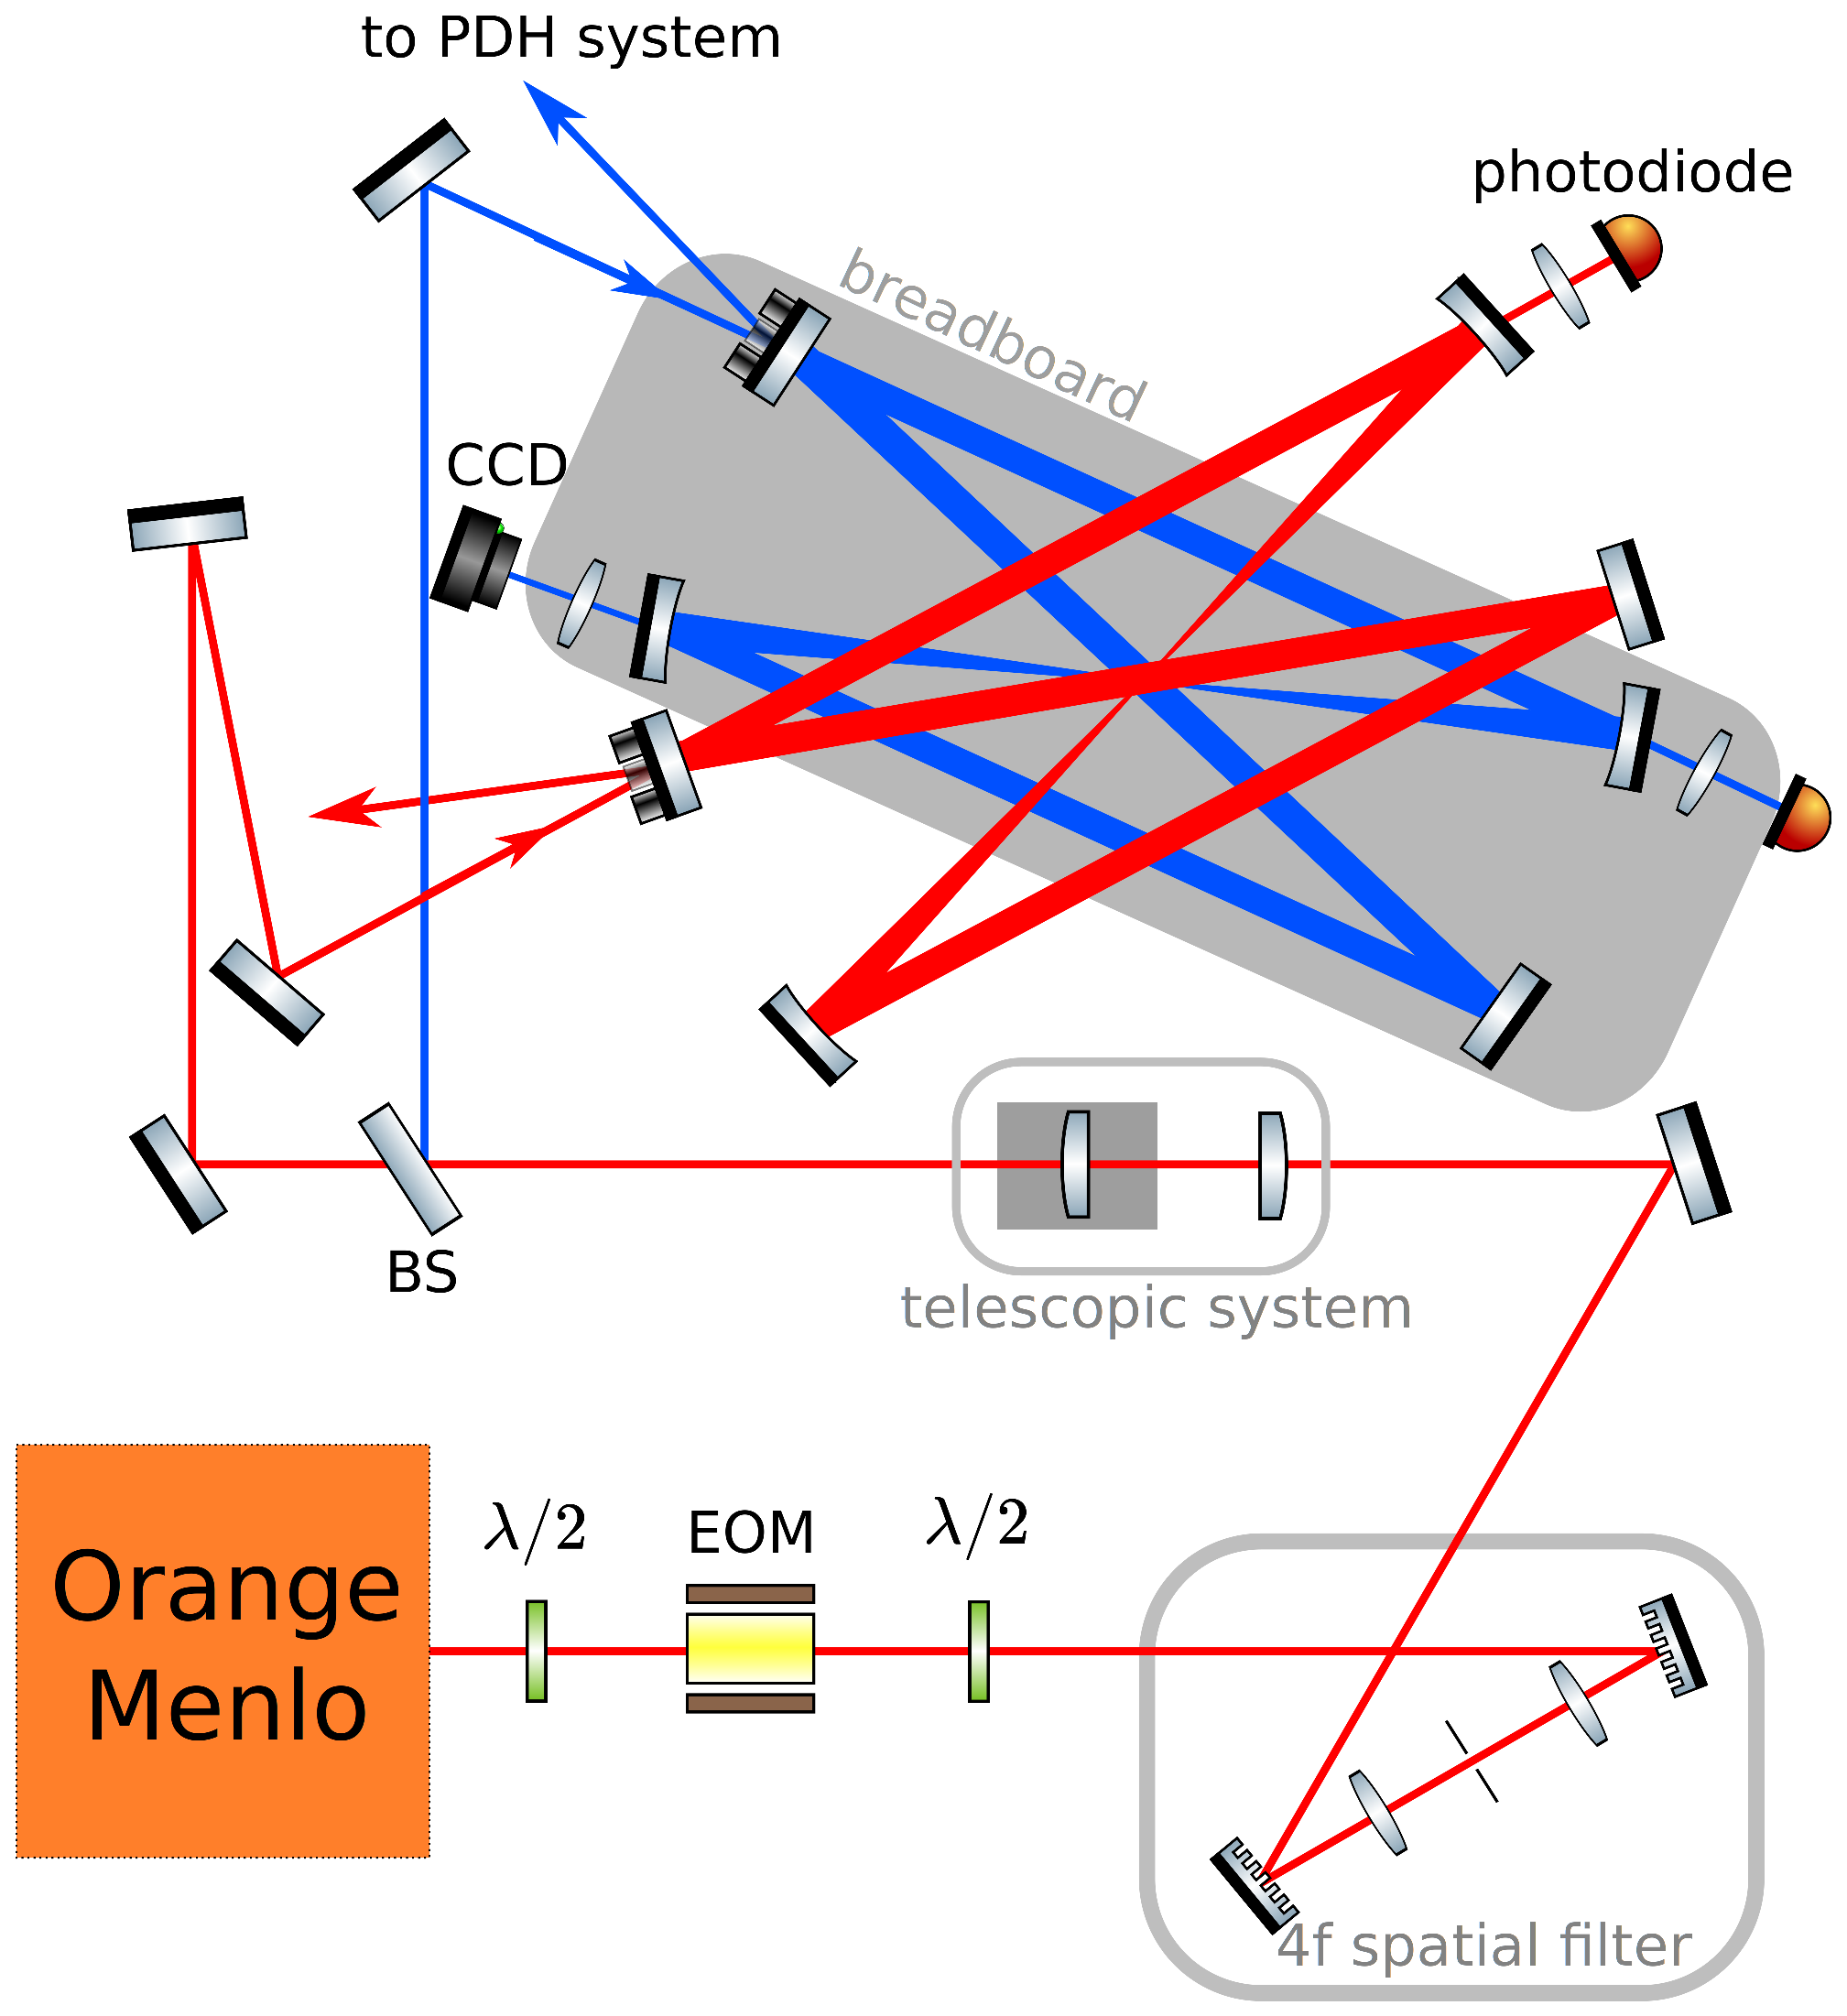
\includegraphics[width=1\linewidth]{images/schema.eps}
	\caption{The experimental setup. The 4f spatial filter consists in two diffraction gratings (1200 lines/mm) and two lenses ($f=100$\,mm), different frequencies focalize at different transverse positions and are selected by a slit between the lenses. The telescopic system can be adjusted by moving one of the lenses with a sled. Different colors are used only to highlight the two cavities. The transmitted beams are monitored with photodiodes and a CCD camera. The reflected beams are used by the two stabilization systems (see Fig \ref{fig:pdh}).}
	\label{fig:schema}
\end{figure}
\begin{figure}
	\centering
	\includegraphics[width=1\linewidth]{images/setup.jpg}
	\caption{The two crossed optical cavities realized in our laboratory.}
	\label{fig:setup}
\end{figure}
The Menlo Orange oscillator and the cavities are placed on an optical table covered with a laminar flow hood. The pulses exiting the laser source pass through an electro-optic modulator to generate two 3.5\,GHz sidebands around the carrier frequency, needed for the PDH system. Then it goes through a 4f spatial filter used to regulate the spectral width of the beam entering the cavities, a reduced spectrum improves the spectral coupling with the cavity but reduces the laser pulse power: a good compromise for the current cavities is a bandwidth with $\Delta\lambda = 3\,$nm.
The polarization is controlled with half-wave plates. A telescopic system with two lenses ($f_1 = f_2= 75$\,mm) is used to regulate the beam radius $w$ and its divergence to ensure maximum spatial coupling with the resonators. A beam splitter divides the pulse in order to seed both cavities.

\subsection{Bow-tie cavities}

Currently the two cavities are very different since the R\&D program proceeds step by step: the $\alpha = 7\degree$ cavity (from hereafter ``blue cavity'') is the more advanced one while the $\alpha = 30\degree$ cavity (the ``red cavity'') is a precedent prototype that was built in the program.

The blue cavity is composed of dielectric mirrors with high reflectivity\footnote{Ther mirrors are from Layertec company, the nominal reflectivity is $>0.99995$ for mirrors B C D, we later found the total reflectivity by measuring the mirror finesse and the coupling efficiency.}, the expected Finesse is about 770. The curved mirrors have a nominal radius of curvature of 750\,mm. The mirrors are mounted on a breadboard to reduce the mounting heights and to decouple the mirror oscillations from the optical table oscillations. The input coupler has a nominal reflectivity of 99.2\%, giving an expected enhancement factor of about 480; it is mounted on the piezo ring crystal used by the stabilization system. A piezo-controlled positioning system by SmarAct (Fig \ref{fig:smaract}) is used for aligning the cavity and finding the exact cavity length to satisfy the temporal condition, but also for the spot size compensation method and for moving the cavity waist.
\begin{figure}
	\centering
	\includegraphics[width=0.9\linewidth]{images/smaract.png}
	\caption{The SmarAct tilting mirror and the SmarAct positioning stage used for the alignment of the cavity and the moving of the beam waist.}
	\label{fig:smaract}
\end{figure}
To align the external beam with the cavity axis ray two mirrors outside the cavity are used, one of which is the beam splitter. The transmitted beams are used to monitor the power inside the cavity and for imaging purposes, while the reflected beam is used by the stabilization system.

The red cavity mirrors have lower reflectivities, giving a Finesse of about 410. The radius of curvature of the curved mirrors has been measured to be $R_B = 767$\,mm and $R_C = 741$\,mm.

The total cavity length is the same for both cavities and equal to 2990\,mm.

\subsection{The PDH stabilization systems}
\begin{figure}
	\centering
	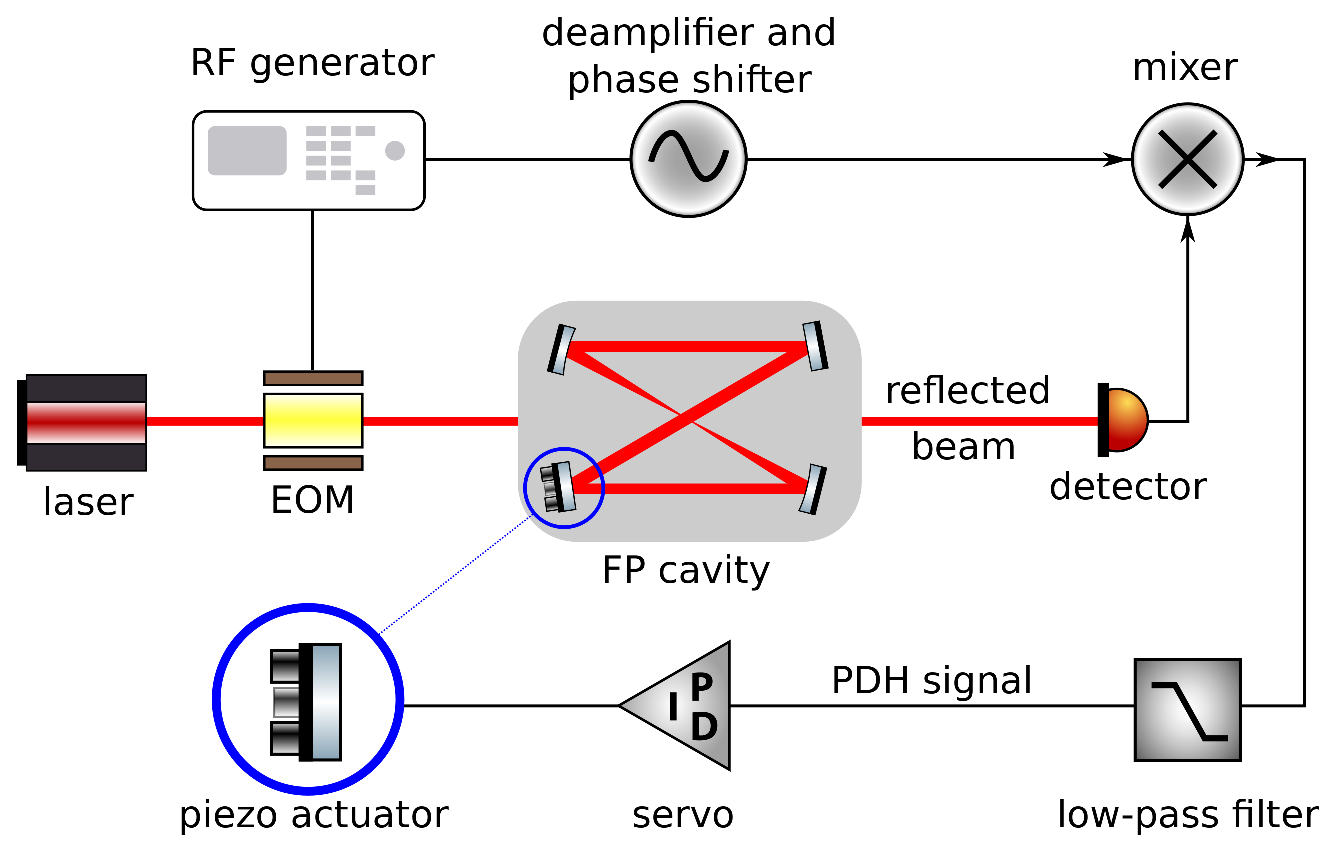
\includegraphics[width=1\linewidth]{images/pdh.eps}
	\caption{The PDH stabilization system scheme. The RF generator drives the EOM with a 3.5\,GHz sinusoidal wave to produce the sidebands. The reflected power signal (in which the sidebands and the carrier wave interfere) is demodulated with the same sinusoidal wave (controlled in phase and amplitude). After a pass through a 6th order Butterworth low-pass filter we have the PDH error signal (Fig \ref{fig:pdhtra}). The error signal is fed through a servo PID that then drives the actuator inside the cavity, adjusting the length and maintaining the stabilization with the external laser source.}
	\label{fig:pdh}
\end{figure}
The stabilization systems (one for each cavity) are composed by an electro optic modulator, a detector, a phase shifter, a mixer and a filter that togheter form the discriminator that produces the error signal. The signal is then fed to a servo PID\footnote{Only the integral and proportional stages are present in our system.} that drives the piezo actuator. The scheme is represented in Fig \ref{fig:pdh}.

\subsubsection{Stabilization procedure}

Here is the procedure we followed to stabilize the cavities and make them resonate:
\begin{enumerate}
	\item We align the cavity and the external mirrors by making sure the beam superimposes with itself after a round-trip.
	\item We send a triangular wave to the piezo to scan the cavity and we monitor the transmitted power searching for the resonance.
	\item We adjust the cavity length using the sleds until resonance is achieved, when this happens we see spikes in the transmitted power corresponding to different modes that resonate in the cavity (as in Fig \ref{fig:goodspa}).
	\item Using the external mirrors, the input coupler and the telescopic system we optimize the spatial coupling efficiency, maximizing the power coupled with the $HG_{00}$ mode and minimizing that coupled with other modes.
	\item We monitor the reflected power and the error signal and optimize its shape acting on the phase shifter (Fig \ref{fig:pdhtra}).
	\item We stop the scanning triangular wave and we search for the resonance by acting manually on the piezo voltage.
	\item Around resonance we activate the integral and the proportional stages to lock the cavity.
	\item The cavity is now stabilized, to optimize the parameters of the PID (integrator and proportional gain and the filter cut-off frequency) we look at the integrated spectral noise on the oscilloscope, minimizing it.
\end{enumerate}
\begin{figure}
	\centering
	\includegraphics[width=1\linewidth]{images/pdhtra.eps}
	\caption{The PDH error signal produced by the discriminator during a cavity scan.}
	\label{fig:pdhtra}
\end{figure}
\begin{figure}
	\centering
	\includegraphics[width=0.5\linewidth]{images/foto/fotodiodo.jpg}
	\caption{The Thorlabs photodiode used to monitor the blue cavity transmitted beam.}
	\label{fig:fotofotodiodo}
\end{figure}

\section{Experimental measurements}

\subsection{Cavity Finesse measurement}
\begin{figure}
	\centering
	\includegraphics[width=0.9\linewidth]{images/FSRfinesse.eps}
	\caption{Finesse measurement by monitoring the transmitted power during a piezo scan of the cavity. Top: scan of a FSR of the cavity ($\delta L > 1030$\,nm), the two peaks correspond to $HG_{00}$ modes resonating inside the cavity. Bottom: scan of a single transmission peak, its width corresponds to the cavity linewidth. The deformation on the peak is due to noise on the scanning piezo.}
	\label{fig:FSRfinesse}
\end{figure}
The resonator Finesse, defined in eq. \ref{eq:finesse}, depends on the cavity losses and can be directly measured by measuring the cavity linewidth and the Free Spectral Range of the cavity. We recall that the power transmitted by the power depends on the detuning $\delta = 2\pi (\nu-\nu_0)L/c$ via eq \ref{eq:power}, so to find the cavity linewidth we can scan the cavity length using the piezo. In Fig \ref{fig:FSRfinesse} we see the transmitted power during a scan, the distance between two peaks corresponds to a change in cavity length of $\lambda = 1030$\,nm. The Finesse can be obtained by dividing the temporal interval between two peaks by the temporal FWHM of a peak. The peak shape must be optimized: if the scanning frequency is too low the piezo is subject to disturbances and noises that deform the peak shape, if it is too high the cavity might not reach the internal maximum power due to its higher characteristic time. The peak shape is then fitted with a Airy function (Fig \ref{fig:FSRfinesse}) to get the cavity linewidth, the result for the blue cavity is:
\begin{align}
	\mathrm{Finesse} = \frac{\nu_{\mathrm{FSR}}}{\delta\nu} =\frac{t_{\mathrm{FSR}}}{\delta t} = \frac{0.1922\,s}{(2.55\pm 0.10)\times 10^{-4}\,s} = 752 \pm 30
\end{align}
Where the error on the measurement is taken to be the difference in FWHM between the acquired data and the Airy function fit. 
The Finesse for the red cavity is instead measured to be $F = 406\pm25$.
\subsection{Power Spectral Density Noise measurement}

\begin{figure}
	\centering
	\includegraphics[width=0.9\linewidth]{images/PSD.eps}
	\caption{Power Spectral Density of the frequency noise between the blue cavity and the laser source. Top: full spectrum of the PSD, the broad peak at 10000\,Hz is due to the PDH system auto-oscillations. Bottom: low frequency spectrum of the PSD, each peak corresponds to a different mechanical harmonic oscillator in the system, such as the mirror mountings.}
	\label{fig:PSD}
\end{figure}
\begin{figure}
	\centering
	\includegraphics[width=0.9\linewidth]{images/rossabroad.eps}
	\caption{Power Spectral Density noise for the red cavity. The noise is much higher and primarly due to the low-frequency peak at 150\,Hz.}
	\label{fig:rossabroad}
\end{figure}

The cavity-laser system is subject to a variety of noise sources, from pump fluctuations in the oscillator to mechanical vibrations of the mirrors. These effects contribute to the cavity-laser detuning and are taken care by the stabilization system. To quantify this noise and describe it in the spectral domain a Power Spectral Density (PSD) noise measurement can be made. The PSD of a signal $x(t)$ is defined as
\begin{align}
	S(f) = \lim_{T\rightarrow\infty}\mathrm{E}\left[|\tilde x(f)|^2\right]
\end{align}
where E denotes the expected value and $\tilde x(f)$ is the truncated Fourier transform of $x(t)$:
\begin{align}
	\tilde x(f) = \frac{1}{\sqrt{T}} \int_{0}^{T}x(t) e^{-i2\pi ft} dt
\end{align}
Another equivalent definition is the Fourier transform of the autocorrelation function of the signal:
\begin{align}
	S(f) = \int_{-\infty}^{\infty} R(\tau) e^{-i2\pi\tau f} d\tau
\end{align}

We are interested in the frequency noise between the stabilized cavity and the laser source, since the PDH system works by translating a frequency noise difference in an asymmetric signal we can use the error signal generated by the discriminator to monitor the frequency noise and calculate its PSD.

The experimental procedure consists in the following steps:
\begin{enumerate}
	\item The cavity is stabilized as described earlier in the chapter, the stabilization parameters are optimized looking at the integrated noise on the oscilloscope.
	\item The error signal coming out of the mixer is sent to the oscilloscope and the signal is acquired on a 0.5\,s temporal window.
	\item The trace of the oscilloscope is acquired ten times while the cavity remains stabilized.
	\item To acquire the background signal the cavity is disrupted by blocking the ray inside it. The background signal is also acquired ten times.
	\item To obtain the frequency/voltage conversion factor ($k$) of the system the error signal is analyzed: we know the two sidebands are separated by 7\,MHz and from this the linear coefficient of the ``linear zone'' can be inferred.
	\item The data is analyzed by taking the PSD of each measurement, averaging them and subtracting the average PSD background.
\end{enumerate}

Results for the blue cavity are shown in Fig \ref{fig:PSD}, noise at low-frequencies is due mainly to mechanical vibrations while electronic noise, such as auto-oscillations of the stabilization system, is at high-frequencies. The integrated noise $\sigma$ corresponds to the $\sigma_{\mathrm{RMS}}$ of the error signal in the time domain. For the power inside the cavity to remain stable, this integrated noise must be much less than the cavity linewidth, in our case:
\begin{align}
	\frac{\sigma}{\delta\nu} = \frac{3500\,\mathrm{Hz}}{130000\,\mathrm{Hz}} \approx 0.027 \ll 1
\end{align}
Note that if we increase the cavity Finesse the integrated noise must be kept smaller to ensure good cavity stabilization, for this reason the PSD noise is used as a benchmark in the R\&D system: most upgrades (such as better and lower mountings and the breadboard) are finalized to reduce the cavity noise.

\subsection{Spatial and spectral coupling}

As noted before, good spatial and spectral coupling between the cavity fundamental mode and the outside laser mode must be achieved to ensure maximum power is reached inside the cavity. Spatial coupling can be optimized acting on the laser beam with a telescopic system and mirrors, ensuring its transverse profile matches that of the cavity fundamental mode (i.e. the overlap integral must be maximized). Spectral coupling is affected mainly by two factors: the laser source Carrier-Envelope-Offset and the mirror dispersion, the former can be controlled acting on the source with a stabilization system (not currently present in our setup) while the latter depends only on the nature of the cavity mirrors. In both cases by reducing the spectral width of the pulse incident on the cavity the spectral coupling can be increased.

\subsubsection{Spatial coupling}
\begin{figure}
	\centering
	\includegraphics[width=0.9\linewidth]{images/goodspa.eps}
	\caption{Transmitted power in the cases of bad (top) and good (bottom) spatial coupling. When the spatial coupling is good only $HG_{00}$ modes resonate in the cavity (those separated by a FSR), when it is bad additional modes (usually first or second order modes) can resonate and other transmission peaks can be seen.}
	\label{fig:goodspa}
\end{figure}

The spatial coupling is quantified by the normalized overlap integral
\begin{align}
\frac{P_\mathrm{coupled}}{P_\mathrm{ext}} = \frac{	\left|\bra{\phi_\mathrm{ext}}\ket{\phi_{00}}\right|^2} {\bra{\phi_\mathrm{ext}}\ket{\phi_\mathrm{ext}}}
\end{align}
where $P_\mathrm{coupled}$ is the power coupled inside the cavity, $P_\mathrm{ext}$  is the total power incident on the cavity, $\ket{\phi_\mathrm{ext}}$ is the external laser mode and $\ket{\phi_{nm}}$ are the normalized cavity Hermite-Gauss modes. Since the Hermite-Gauss modes form a complete system and are orthogonal to each other we can write
\begin{align}
	\frac{P_\mathrm{coupled}}{P_\mathrm{ext}} = \frac{	\left|\bra{\phi_\mathrm{ext}}\ket{\phi_{00}}\right|^2} {\sum_{nm}\left|\bra{\phi_\mathrm{ext}}\ket{\phi_{nm}}\right|^2}
\end{align}

The power inside the cavity $P_\mathrm{in}$ (and the transmitted power) is directly proportional to the power coupled
\begin{align}
	P_\mathrm{in} \propto P_\mathrm{coupled} \propto \left|\bra{\phi_\mathrm{ext}}\ket{\phi_{00}}\right|^2
\end{align}
This means that by measuring the power transmitted by the cavity when each mode $\ket{\phi_{nm}}$ oscillates we can calculate the spatial coupling with the fundamental mode
\begin{align}
		\frac{P_\mathrm{coupled}}{P_\mathrm{ext}} = \frac{P_{00}}{\sum_{nm} P_{nm}}
\end{align}
where $P_{nm}$ is the power transmitted by the cavity when the mode $HG_{nm}$ is resonating.

To measure the transmitted power for each mode we scan the cavity with the piezo, the scanning time must be compatible with the characteristic cavity time to ensure maximum power is reached inside the cavity. The height of each transmission peak gives the transmitted power for the corresponding mode, we only need to measure the height of the peaks between two $HG_{00}$ modes since the pattern repeats itself every Free Spectral Range. In Fig \ref{fig:goodspa} we can see both cases of bad and good spatial coupling. The measurements indicate a spatial coupling of about 90\%.

\subsubsection{Spectral coupling}
\begin{figure}
	\centering
	\includegraphics[width=0.9\linewidth]{images/mephisto.eps}
	\caption{Thorlabs CCD spectrometer calibration. The incident light is produced by a ultra-narrow bandwidth 1064\,nm CW laser. The FWHM, taken as instrument resolution, is $\delta\lambda = 1.2$\,nm. The broadening at the base is due to the multi-mode fiber propagation.}
	\label{fig:mephisto}
\end{figure}

To obtain the spectral coupling we can measure the spectrum of the radiation incident on the cavity and compare it with that of the transmitted radiation. For the measurement we used a CCD spectrometer from Thorlabs, the beam is sent to the spectrometer through an optical fiber. Good coupling with the fiber must be achieved in order to not alter the measured spectrum by pumping lateral modes of the multi-mode fiber. For this we used the fiber coupler shown in Fig \ref{fig:coupler}, which includes a converging lens.

\begin{figure}
	\centering
	\includegraphics[width=0.8\linewidth]{images/foto/coupler.jpg}
	\caption{The fiber coupler used for the measuring of the laser beam spectra, two such couplers has been used: one before the cavity and one after. At the center there is a converging lens, while the fiber is attached on the back, the regulation is done through two screws.}
	\label{fig:coupler}
\end{figure}

We first estimated the instrument spectral resolution by measuring the spectrum produced by a CW ultra-narrow linewidth laser (the Mephisto ND:YAG laser), the spectrometer response is shown in Fig \ref{fig:mephisto}, this response can be used to deconvolute the measurements to increase precision. It is worth to note that the response has been measured at 1064\,nm while the other measurements occur at 1030\,nm, where the instrument response could be different. From this we get a resolution of about $\delta \lambda =1.2$\,nm.

The procedure to acquire the radiation spectra consists in the following steps:
\begin{enumerate}
	\item The laser beam power is measured outside the cavity with a photodiode.
	\item The beam is coupled with a fiber coupler, the coupling is optimized until 85-90\% of the power is transmitted through the fiber.
	\item The fiber is connected to the spectrometer, the power must be reduced using optical filters not to saturate or damage the instrument.
	\item The input spectrum is acquired.
	\item The cavity is stabilized, and the transmitted beam is coupled in the fiber, again optimizing the power coupling.
	\item The output spectrum is acquired.
	\item The input and output spectrum are renormalized in intensity and their integrated profile compared to calculate the spectral efficiency.
\end{enumerate}

The first measurement has been done on the blue cavity with Finesse 750 (as shown earlier the coupling can depend on the Finesse).
The results, shown in Fig \ref{fig:6nm}, demonstrate that our instrument has a resolution too small to differentiate between the input and output spectrum, as they appear to be about the same width in both cases (6\,nm input and 10\,nm input).
Another factor that may obscure the difference is that the coupling with the fiber may be different between the two measures. Within the resolution of our instrument, we can say that the spectral coupling efficiency is very high ($>85\%$). According to the results of the next section regarding mirror reflectivities, the coupling efficiency is even higher.

\begin{figure}
	\centering
	\includegraphics[width=0.9\linewidth]{images/6nm.eps}
	\caption{Spectra for the radiation incident on the cavity and transmitted by the cavity. The difference is too small if confronted with the spectrometer resolution so the spectra appear similar.}
	\label{fig:6nm}
\end{figure}

To demonstrate that the experimental procedure is correct, we can change the $f_\mathrm{CEO}$ and verify that the spectral coupling changes with it (as shown earlier, Fig \ref{fig:couplingeta}). Note that we can't directly control the offset, but since it depends on the temperature of the lasing medium, we can change it by varying the laser diode current. In Fig \ref{fig:currents} we can see that the radiation spectrum at the output depends strongly on the diode current. In this case the coupling with the fiber remains the same, since the apparatus is the same for all measures, and the differences in the transmitted radiation spectra are more evident.

\begin{figure}
	\centering
	\includegraphics[width=0.9\linewidth]{images/currents.eps}
	\caption{Different transmitted spectra obtained by changing the Menlo laser diode current. The change in current translate to a change in temperature in the active medium, this changes the $f_\mathrm{CEO}$ and so the spectral coupling (see Fig \ref{fig:couplingeta}). In this case the best spectral coupling is obtained for 500\,mA.}
	\label{fig:currents}
\end{figure}

We then replaced the input coupler, going from 99.2\% reflectivity to about 99.8\% and increasing the cavity Finesse to about 3000.
We again measured the spectral coupling, changing the oscillator diode current. This time we were able to measure a spectral coupling efficiency of about 90\% for all cases, the improvement is probably due to better fiber coupling. The results are shown in Fig \ref{fig:accspe} and Tab \ref{tab:coup3000}. The differences between the measurement are due to a different value for the $f_\mathrm{CEO}$.

\begin{figure}
	\centering
	\includegraphics[width=0.9\linewidth]{images/accspe.eps}
	\caption{Different transmitted spectra for the Finesse 3000 cavity. In this case the best spectral coupling is obtained for 480\,mA.}
	\label{fig:accspe}
\end{figure}
\begin{table}
	\centering
	\begin{tabular}{|c|c|c|c|}
		\hline 
		current [mA]&spectral coupling & $P_\mathrm{ref}/P_\mathrm{in} $ & Mirrors reflectivity\\ 
		\hline 
		505	& $0.9\pm5$ & 0.62 & $0.99996 \pm0.00005$ \\ 
		\hline 
		530	& $0.91\pm5$ & 0.65 & $0.99998 \pm0.00005$\\ 
		\hline 
		550	& $0.91\pm5$ & 0.65 &$0.99998 \pm0.00005$ \\ 
		\hline
		480	& $0.96\pm5$ & 0.56 &$0.99983 \pm0.00005$ \\ 
		\hline
		505	& $0.91\pm5$ & 0.56 &$0.99990 \pm0.00005$ \\ 
		\hline
	\end{tabular}
	\caption{Spectral coupling for the blue cavity at Finesse 3000. The reflected power is used to calculate mirror reflectivities. The error on the spectral coupling is given by the instrument resolution (Fig \ref{fig:mephisto}), and that on the reflectivity by error propagation. The measurement at 480\,mA gives an efficiency higher than the others that results in a lower reflectivity. The other measurements are compatible with a reflectivity of 99.995\% for mirrors B C and D.}
	\label{tab:coup3000}
\end{table}

\subsubsection{Mirror reflectivities}

If we consider spatial and spectral coupling efficiencies $\eta_1$ and $\eta_2$ in calculating the power reflected by the cavity when in resonance (eq. \ref{eq:ref}), we get
\begin{align}
\frac{P_\mathrm{ref}}{P_\mathrm{in}} = \left[ \frac{\sqrt{\eta_1\eta_2}(1-R_1)\sqrt{R_2R_3R_4}}{1-\sqrt{R_1R_2R_3R_4}}-\sqrt{R_1}  \right]^2
\end{align}
From the equation we can see that by measuring the reflected power when the cavity is stabilized, and by knowing the efficiencies, we can estimate the total mirrors reflectivity $R_2R_3R_4$. For this purpose, we consider the reflectivity of the input coupler $R_1$ to be that indicated by the supplier (Layertec): $99.25\%$ (this is in accordance with the Finesse measurement). The previous Finesse measurement gives a minimum reflectivity of about 99.98\% for each mirror\footnote{The Finesse provides only a minimum figure because other losses contribute to the Finesse measured value.}.

To measure the reflectivities we then proceed as follows:
\begin{enumerate}
	\item The input radiation spectrum is acquired, following the steps described earlier.
	\item The reflected power (out of resonance) is measured.
	\item The spatial coupling efficiency is calculated looking at the transmission peaks.
	\item The cavity is stabilized.
	\item The transmitted radiation spectra is acquired.
	\item The reflected power (in resonance) is measured.
	\item The spectra are confronted to estimate the spectral coupling efficiency.
\end{enumerate}

The measurement of the spectral coupling efficiency $\eta_2$ is not precise, but using the other data we can plot (Fig \ref{fig:reflectivities}) the mirror reflectivities $R$ ($R=R_2=R_3=R_4$) as a function of $\eta_2$. From the plot we can see that $\eta_2$ must be over 92\%. The two measurements are compatible with a mirror reflectivity around 99.995\% estimating $\eta_2$ at 95\%.

The calculation has also been made with the results obtained using the coupler with 99.8\% reflectivity, but since we weren't able to accurately measure the Finesse of the cavity we cannot yet trust the nominal reflectivity value (new methods for measuring the Finesse are being developed in our laboratory). The results assuming the mirror A nominal reflectivity are in Tab \ref{tab:coup3000}.
\begin{table}
	\centering
	\begin{tabular}{|c|c|c|}
		\hline 
		data  &$P_\mathrm{ref}/P_\mathrm{in}$ &$\eta_1$ \\ 
		\hline 
		6\,nm	& 0.59 & 89\% \\ 
		\hline 
		10\,nm	& 0.67 & 90\% \\ 
		\hline 
		
	\end{tabular}
	\caption{Data points for the mirror reflectivity measurements. $\eta_1$ is the spatial coupling efficiency.}
	\label{tab:ref}
\end{table}

\begin{figure}
	\centering
	\includegraphics[width=0.9\linewidth]{images/reflectivities.eps}
	\caption{Mirror reflectivity for different values of the spectral coupling efficiency. The two colors indicate two different measurements (data in Tab \ref{tab:ref}). If we estimate $\eta_2$ to be about 95\% the measurements are compatible with a mirror reflectivity of 99.995\%.}
	\label{fig:reflectivities}
\end{figure}

\subsection{Compensation method}

As explained earlier, the compensation method will be used to address the issue of thermal deformation of the mirrors at high power. The measurement is available thanks to the piezo-driven linear stages represented in Fig \ref{fig:smaract}.

The sleds can move in two different ways, named scan mode and step mode. When in scan mode, the voltage on the piezo is directly controlled (from 0\,V to up to 100\,V). In step mode, the piezo is subjected to an alternate voltage and undergoes several cycles of stretching and contracting, resulting in an overall movement in the specified direction\footnote{This technology is called ``Stick-Slip Drive'', further details can be found at \url{https://www.smaract.com/technology-introduction-and-options}.}. While the sled can move macroscopically in step mode, the distance covered in scan mode is given only by the piezo crystal properties and amounts to $\approx 0.5\,\mu$m.

Two sleds are needed to change the distance between the curved mirrors and to restore the cavity length. An application written in LabView has been developed to move both the sleds at the same time. We have verified that movement in step mode is not possible, as the stabilization system is not able to correct for the sudden changes in cavity length, while this doesn't happen for a movement in scan mode. To achieve the distances required by the correction (that are on the order of a millimeter, Fig \ref{fig:compensation}) a new kind of long-distance moving piezo driven mirror mounting is been developed and characterized.

The experimental procedure consists in:
\begin{enumerate}
	\item placing the sled in the correct position for the movement (since they must go in opposite ways, one can be placed at 0\,V while the other at 100\,V)
	\item locking the cavity using the stabilization system
	\item moving the sleds simultaneously 
\end{enumerate}
\begin{sidewaysfigure}
	\centering
	\includegraphics[width=0.9\linewidth]{images/smaractmove.pdf}
	\caption{Moving the piezo-driven sleds in the stabilized cavity. The first two rows show the effect of moving a single sled, the PDH piezo corrects the change in cavity length and maintains the transmitted beam stable. The last row show the effect of moving both at the same time: tha cavity length is unchanged.}
	\label{fig:smaractmove}
\end{sidewaysfigure}

The transmitted beam has been monitored to ensure that the stabilization system is fast enough to correct the movements in real time, also the voltage on the piezo used by the stabilization system has been monitored to measure the change in cavity length. The results, shown in Fig \ref{fig:smaractmove}, show that when moving both the sleds the cavity length is unaffected (voltage on PDH piezo is constant), and the transmitted power is unchanged (and so the cavity internal power). By monitoring the voltage on the PDH piezo we can measure that by moving only one sled we change the cavity length of about $430\,$nm, since we know a wavelength ($\lambda = 1030\,$nm) corresponds to a change of about 7\,V on the PDH piezo.

\subsection{Cavity waist movement}

As demonstrated in the theoretical chapter, by inclining the curved mirrors we can move the cavity waist between them, this technique will be used in BriXS to change the cavity that interacts with the electron beam, enabling the dual color mode. To achieve the movement we used piezo-driven tilting mirrors that use the same ``Stick-Slip Drive technology'' as the sleds, again in scan mode.

\subsubsection{Mirror tilting measurement}
\begin{figure}
	\centering
	\includegraphics[width=0.9\linewidth]{images/tiltingme.eps}
	\caption{The apparatus used to measure the voltage-angle relation for the tilting mirrors. The telescopic system is used to collimate the beam. The focal length $f$ of the lens is 500\,mm.}
	\label{fig:tiltingme}
\end{figure}
\begin{figure}
	\centering
	\includegraphics[width=0.8\linewidth]{images/mirrortilt.eps}
	\caption{Voltage-angle relation for the tilting mirrors. The relation is linear, with a max movement of $100\,\mu$rad.}
	\label{fig:mirrortilt}
\end{figure}

To characterize the tilting mirror mountings (i.e. to find the voltage-angle relation) we shine a laser at the mirror and monitor the movement of the beam with a CCD camera, after passing through a lens. The system is shown in Fig \ref{fig:tiltingme}. To relate the movement on the camera sensor with the angular movement we write the ABCD matrix for the system starting on the mirror surface, it is composed by a free space propagation of length $f$, a lens of focal length $f$ and another free space propagation:
\begin{align}
\begin{bmatrix}
1 & f \\
0 & 1 \\
\end{bmatrix}
\begin{bmatrix}
1 & 0 \\
-1/f & 1 \\
\end{bmatrix}
	\begin{bmatrix}
	1 & f \\
	0 & 1 \\
	\end{bmatrix}
	\begin{bmatrix}
	0 \\
	\theta  \\
	\end{bmatrix}
	=
	\begin{bmatrix}
	f\theta \\
	0  \\
	\end{bmatrix}
\end{align}

where $\theta$ is the initial ray inclination given by the tilting mirror. Note that if the ray has inclination $\theta$ that means that the mirror has moved by $\theta/2$.
The measurement gives a linear relation between voltage and angular tilt (Fig \ref{fig:mirrortilt}), with a maximum movement of 100\,$\mu$rad. According to the previous calculation that means that we can achieve a vertical shift of the waist of about 80\,$\mu$m. To achieve the movement required for BriXS (110\,$\mu$m) we are developing a new tilting mounting with a longer stroke. The new mountings will also be gimbal-like to avoid changing the cavity length during the movement.


\subsubsection{Focus movement measurement}

To directly observe the cavity waist during the movement we placed a high transmission plate inside the cavity at the focus location. A small part of the beam is reflected and can be used for an imaging of the focus. To find the waist location inside the cavity we observe the beam shape: since the cavity is astigmatic and near-confocal along the vertical direction its shape will be that of an horizontal ellipsoid near the focus, and that of a vertical ellipsoid away from it.

\begin{figure}
	\centering
	\includegraphics[width=0.8\linewidth]{images/focusima.eps}
	\caption{Apparatus for the imaging of the cavity waist.}
	\label{fig:focusima}
\end{figure}

After placing the imaging system, we can calculate the magnification factor by measuring the CCD-lens distance using
\begin{align}
	M = -\frac{q}{p} && \frac{1}{f} = \frac{1}{p} + \frac{1}{q}
\end{align}
where $p$ and $q$ are the distances of the waist and the camera from the lens, and $f$ its focal length. In our case
\begin{align*}
	p = 286\,\mathrm{mm} &&q = 315\,\mathrm{mm} &&f = 150\,\mathrm{mm} && M = -1.1
\end{align*}
Note that $M$ is negative so the image is inverted. The measured waist size $w$ is
\begin{align*}
	w_\mathrm{H} = 87\,\mu\mathrm{m} && w_\mathrm{V} = 61\,\mu\mathrm{m} 
\end{align*}

The procedure to measure the cavity waist movement consists in stabilizing the cavity, measuring the waist position using the image on the CCD camera, moving mirrors B and C at the same time and then repeating the position measurement.
During the movement we monitored the transmitted power and the PDH piezo voltage, to measure the shortening in cavity length.
In Fig \ref{fig:imagemov} and Fig \ref{fig:tilt} we see the images acquired during a movement and the relative data, the movement has been done applying a mirror tilt of 50\,$\mu$rad in a time of 55\,ms, resulting in a vertical shift of 36\,$\mu$m, in accordance with the predicted value of eq. \ref{fig:shiftfocus}. The transmitted power is unchanged before and after the movement, while during the movement it undergoes fluctuations. As indicated by the tension on the PDH piezo voltage, the cavity length changes by about $2\,\mu$m, corresponding to 14\,V.
\begin{figure}
	\centering
	\includegraphics[width=1\linewidth]{images/imagemov.eps}
	\caption{Imaging of the cavity waist before and after the movement. To measure the beam radius $w$ and the shift the intensity profile has been fitted with a gaussian function.}
	\label{fig:imagemov}
\end{figure}
\begin{figure}
	\centering
	\includegraphics[width=1\linewidth]{images/doublefocus.eps}
	\caption{Waist movement while both cavities are stabilized.}
	\label{fig:doublefocus}
\end{figure}
\begin{figure}
	\centering
	\includegraphics[width=0.9\linewidth]{images/tilt.eps}
	\caption{Top: transmitted power and PDH piezo voltage during the movement. Bottom: vertical intensity profile of the beam waist along the vertical direction, before and after the movement (not corrected with the imaging magnification factor $M$).}
	\label{fig:tilt}
\end{figure}

In Fig we can see the movement of one focus while both the red and blue cavity are stabilized, using the full tilting range of the mirrors the movement is about $80\,\mu\mathrm{rad}$. Only one cavity is currently equipped with the moving mirrors.



The measurement demonstrates the possibility of moving the laser beam of the two BriXS cavities in and out of the interaction point with the electrons, in a very short time ($\sim 100\,$ms) compatible with its medical applications.
	\chapter{Conclusions}

During this thesis work we developed and built two crossed Fabry-Perot optical cavities to be used in the Inverse Compton Scattering source of MariX.

The resonators are actively stabilized against the mode-locked laser source using two independent feedback systems implementing the Pound-Drever-Hall technique. The cavities have been experimentally characterized, regarding their mirror reflectivities, their Finesse, their spatial and spectral coupling with the external laser mode, and their PSD frequency noise.

A new method to avoid unwanted high-power effects in the cavity, such as mirror thermal deformation and degenerate mode coupling, has been theoretically developed and an experimental feasibility test has been conducted, giving positive results. 

We developed a technique to move the waists of the cavities while keeping them stabilized with the laser, to be used in BriXS to generate dual-color X-rays for K-edge subtraction imaging. The experimental results indicate that this solution is feasible, yielding a movement of 80\,$\mu$m in less than 100\,ms.

The main cavity and its stabilization system has been continually upgraded during the work, regarding for example the mountings, the electronics and the mirrors. The PSD frequency noise has been used as benchmark for this upgrades, since we want the lowest possible power fluctuation inside the cavity. The latest cavity model has a Finesse of about 3000, corresponding to a linewidth of 33\,kHz, with an integrated frequency noise of about 3500\,Hz.

The next steps in the R\&D program consist in developing and testing new piezo-driven mirror mountings for both the compensation method and the focus shift method, building a hood enclosure to further reduce the noise and developing a reliable method to identify and damp the mechanical oscillators in the system. Two other R\&D lines are also currently starting: one dedicated to the development of the amplification system, and one dedicated to the RF-guns for the electron bunch production. In particular after the amplification system the power in the cavity will reach high enough levels to directly observe the mentioned high power effects.
	
	\printbibliography
 \end{document}